\documentclass[utf8x,notes,pagenumber,hyperref={pagebackref=true,citecolor=green,bookmarks=true,pdfpagelabels=true}]{beamer} %remove draft when done with tex prep
%\documentclass[notes]{beamer} 
\usepackage{etex}
\usepackage{beamerthemesplit}
\usetheme{PaloAlto} %Hannover, Belin, Warsaw, PaloAlto, Frankfurt, Berkeley  etc

% Itemize breaks compilation: https://tex.stackexchange.com/questions/414419/put-bullets-in-a-block-inside-itemize-environment
\usefonttheme{professionalfonts}
\setbeamertemplate{itemize items}[ball]
\setbeamercolor{block title}{fg=white, bg=blue!70!black}
\setbeamercolor{block body}{fg=black, bg=gray!20}
\setbeamertemplate{blocks}[rounded][shadow=true]

\usepackage{pgfpages}
\usepackage{xcolor}
\definecolor{light-blue}{rgb}{0.95,0.55,.9}
\definecolor{light-red}{rgb}{0.95,0.15,.19}
\mode<handout>{\setbeamercolor{background canvas sidebar}{bg=red!45}}
\setbeamercolor{structure}{fg=light-blue}
\usepackage{bm}
\usepackage{subfloat}
\usepackage{paralist}
\usepackage{subcaption}
\usepackage{amssymb, amsmath}
\usepackage{mathrsfs}
\usepackage[round]{natbib}
\usepackage{algorithm}
\usepackage{algpseudocode}
\bibliographystyle{unsrtnat}
\usepackage[export]{adjustbox}
\usepackage{array,booktabs,tabularx}
\usepackage{tikz}
\usetikzlibrary{shapes,arrows, circuits, patterns, snakes, decorations.pathreplacing}
\usepackage{schemabloc, verbatim}
\usepackage{graphicx}

\usepackage{media9} % for video embeddings
\usepackage{multimedia} % for video embeddings
\usepackage{tcolorbox}
\tcbuselibrary{theorems}
\newcommand{\tcb}[2]
{
 \begin{tcolorbox}[title=\text{#2}]
 #1
 \end{tcolorbox}
}

%\renewcommand\thefootnote{}\footnote{#1}
\definecolor{light-blue}{rgb}{0.30,0.35,1}
\definecolor{light-green}{rgb}{0.20,0.49,.85}
\definecolor{purple}{rgb}{0.70,0.69,.2}

\newcommand{\lb}[1]{\textcolor{light-blue}{#1}}
\newcommand{\bl}[1]{\textcolor{blue}{#1}}

\newcommand{\maybe}[1]{\textcolor{gray}{\textbf{MAYBE: }{#1}}}
\newcommand{\inspect}[1]{\textcolor{cyan}{\textbf{CHECK THIS: }{#1}}}
\newcommand{\more}[1]{\textcolor{red}{\textbf{MORE: }{#1}}}

% FYA
\newcommand{\cmt}[1]{{\footnotesize\textcolor{red}{#1}}}%{#2}
%\newcommand{\note}[1]{\cmt{Note: #1}}
%\newcommand{\todo}[1]{\textcolor{cyan}{TO-DO: #1}}
\newcommand{\review}[1]{\noindent\textcolor{red}{$\rightarrow$ #1}}
\newcommand{\response}[1]{\noindent{#1}}
\newcommand{\stopped}[1]{\color{red}STOPPED HERE #1\hrulefill}

%Text commands
\newcounter{mnote}
\newcommand{\marginote}[1]{\addtocounter{mnote}{1}\marginpar{\themnote. \scriptsize #1}}
\setcounter{mnote}{0}
% \newcommand{\comment}[1]{}
\newcommand{\ie}{$i.e.$\ }
\newcommand{\eg}{e.g.\ }
\newcommand{\cf}{c.f.\ }
\newcommand{\yes}{\checkmark}
\newcommand{\no}{\ding{55}}

%Reference commands
\newcommand{\flabel}[1]{\label{fig:#1}}
\newcommand{\seclabel}[1]{\label{sec:#1}}
\newcommand{\tlabel}[1]{\label{tab:#1}}
\newcommand{\elabel}[1]{\label{eq:#1}}
\newcommand{\alabel}[1]{\label{alg:#1}}
\newcommand{\fref}[1]{\cref{fig:#1}}
\newcommand{\sref}[1]{\cref{sec:#1}}
\newcommand{\tref}[1]{\cref{tab:#1}}
\newcommand{\eref}[1]{\cref{eq:#1}}
\newcommand{\aref}[1]{\cref{alg:#1}}

\newcommand{\bull}[1]{$\bullet$ #1}
\newcommand{\argmax}{\text{argmax}}
\newcommand{\argmin}{\text{argmin}}
\newcommand{\mc}[1]{\mathcal{#1}}
\newcommand{\bb}[1]{\mathbb{#1}}


\def\tidx{t}
%\def\comment
%\def\value{V}
% from https://www.cs.jhu.edu/~jason/advice/write-the-paper-first.html
\newcommand{\Note}[1]{}
\renewcommand{\Note}[1]{\hl{[#1]}}  % comment out this definition to suppress all Notes
%\algnewcommand\algorithmicforeach{\textbf{for each}}
%\algdef{S}[FOR]{Foreach}[1]{\algorithmicforeach\ #1\ \algorithmicdo} %

%\newcolumntype{M}[1]{>{\centering\arraybackslash}m{#1}}
\def\coriolis{\textbf{\textit{C}}}
\def\massinertia{\textbf{\textit{M}}}
\def\torque{\bm{\tau}}
\def\frictionvec{\textbf{\textit{f}}}
\def\Smat{\textbf{\textit{S}}}
\def\Bmat{\textbf{\textit{B}}}
\def\wheelrad{\textbf{\textit{r}}}

\def\stateweight{\textbf{\textit{w}}_x}
\def\actionweight{\textbf{\textit{w}}_u}
\def\advactionweight{\textbf{\textit{w}}_v}

%Thesis defs
%\def\upchi{\textchi}
\def\kau{\mc{K}}
\def\particle{\bm{x}}
\def\deformationgrad{\textbf{F}}
\def\refconf{\bm{\upchi}_0}
\def\refconfbody{\mathscr{B}_0}
\def\conf{\bm{\upchi}}
\def\currconf{\bm{\upchi}}
\def\Eulerian{\mc{E}}
\def\cauchystress{\bm{\sigma}}
\def\stresscomp{\sigma}
\def\currconfbody{\mathscr{B}}
\def\materialresponse{\textbf{G}}
\def\orthoggroup{{\textit{SO}}(3)}
\def\liegroup{{\textit{SE}}(3)}
\def\liealgebra{\mathfrak{se}(3)}
\def\identity{\textbf{I}}
\newcommand{\trace}[1]{\textbf{tr}(#1)}
\def\leftcauchy{\textbf{B}}
\def\rightcauchy{\textbf{C}}
\def\fiber{\textbf{dx}}

\def\dof{\text{DOF }}
\def\dofs{\text{DOFs }}
\def\reline{\mathbb{R}}
\def\curve{\deformationgrad}
\def\twist{{\xi}}
\def\contactforce{\tilde{F}}
\def\contactforcecomp{f}
\def\gaussianmap{\textbf{}n}
\def\contacttorquecomp{\tau}
\def\wrt{with respect to }
\def\curveparam{\position}
\def\basis{\bm{e}}
\def\pose{{g}}
\def\selmap{{B}}
\def\manipmap{{G}}
\def\jacob{\bm{J}}
\def\normal{\bm{n}}
\def\position{\textbf{r}}
\def\deformationgradcur{\textbf{H}}
\def\eulerianvel{\textbf{v}(\position, t)}
\def\headparam{\zeta}
\def\strain{\mathrm{\Psi}}
\def\strainiso{\mathrm{\Psi_{\text{iso}}}}
\def\strainfiber{\mathrm{\Psi_{\text{mesh}}}}

% mechanism defs
\def\wallthickness{1cm}
\def\sorodiam{9 cm}
\def\sorodiamdim{5-6.25cm}

% inline macros
\newcommand{\putsoro}[2]{\includegraphics[width=.45\columnwidth,height=#2\columnwidth]{../../../PhDThesis/figures/#1}}
\newcommand{\sorowidth}{.35}


%\newtheorem{theorem}{Theorem}[]
%\newtheorem{example}{Example}
%\newtheorem{homework}{Homework}

\tikzstyle{block} = [draw, fill=yellow!80, rectangle,minimum height=3em, minimum width=4em]
\tikzstyle{sum} = [draw, fill=white!20, circle, node distance=1cm]
\tikzstyle{input} = [coordinate]
\tikzstyle{output} = [coordinate]
\tikzstyle{pinstyle} = [pin edge={to-,thin,black}]

\newcolumntype{Z}{>{\centering\arraybackslash}X} % centered tabularx columns
\newcommand{\pphantom}{\textcolor{ta3aluminium}} % phantom
%\setbeamerfont{title}{shape=\itshape,family=\rmfamily}
\setbeamercolor{title}{fg=magenta!70!black,bg=yellow!70!white}
%
\title{\small A short treatise on robots' kinematic geometry and kinetics.}

\author{Author: Lekan Molu}
\institute{
	%
	\vspace{0.5em}
	%
	Dissemination Venue: Microsoft Research RL Group, \\
	New York City, NY 10012 
}

%\date{\today} 
\date{June 09, 2022} 


\setbeamersize{sidebar width left=2cm}
%remove title and author names from sidebar
  \makeatletter
\setbeamertemplate{sidebar \beamer@sidebarside}%{sidebar theme}
{
	\beamer@tempdim=\beamer@sidebarwidth%
	\advance\beamer@tempdim by -6pt%
	\insertverticalnavigation{\beamer@sidebarwidth}%
	\vfill
	\ifx\beamer@sidebarside\beamer@lefttext%
	\else%
	\usebeamercolor{normal text}%
	\llap{\usebeamertemplate***{navigation symbols}\hskip0.1cm}%
	\vskip2pt%
	\fi%
}%
\makeatother

\begin{document}
	\maketitle
%http://tug.ctan.org/macros/latex/contrib/beamer/doc/beameruserguide.pdf#subsection.21.3
\begin{frame}[allowframebreaks]{Outline}
	\frametitle{Table of Contents}
	\tableofcontents
\end{frame}

\lecture{Bibliography}{Lecture Nut}
\section{Introduction}

\setbeamertemplate{blocks}[rounded][shadow=true]
\subsection{Textbooks}
\begin{frame}
	\frametitle{Standard Texts -- Modeling and Control}
	\begin{block}{Robot Modeling and Control}
		Spong, Mark W., Seth Hutchinson, and Mathukumalli Vidyasagar. Robot modeling and control. Vol. 3. New York: Wiley, 2006.
	\end{block}
	\begin{block}{Mathematical Modeling of Robots}
		Murray, R. M., Li, Z., \& Sastry, S. S. (1994). A Mathematical Introduction to Robotic Manipulation. In Book (Vol. 29). https://doi.org/10.1.1.169.3957
	\end{block}
\end{frame}

\begin{frame}
	\frametitle{Texts -- Modeling, Control, and Mechanisms}
	\begin{block}{Robot Modeling and Control}
		Lynch, K. M., \& Park, F. C. (2017). Modern Robotics Mechanics, Planning, and Control.
	\end{block}
	%
	\begin{tcolorbox}[coltitle=blue!50!black,colframe=blue!25,title=Mechanisms' Kinematic Geometry]
		Hunt, Kenneth H., and Kenneth Henderson Hunt. Kinematic geometry of mechanisms. Vol. 7. Oxford University Press, USA, 1978.
	\end{tcolorbox}
\end{frame}


\begin{frame}
	\frametitle{Texts -- Screws and Kinematics}
	\begin{tcolorbox}[coltitle=blue!50!black,colframe=blue!25,title=Screw Theory]
		Ball, Robert Stawell. A Treatise on the Theory of Screws. Cambridge university press, 1998.
	\end{tcolorbox}
	%
	\begin{tcolorbox}[arc=4mm, 		coltitle=blue!50!black,colframe=blue!25,title=Mechanisms' Kinematic Geometry]
		%
		Hunt, K. H. (2019). Structural Kinematics of In- Parallel-Actuated Robot-Arms. 105(December 1983), 705–712.
	\end{tcolorbox}
\end{frame}

\lecture{Linkages and Mechanisms}{Lecture I}
\section{Pairs, Linkages, and Configurations}

\begin{frame}
	\frametitle{Lecture One Outline}
	\begin{tcolorbox}[coltitle=white!80,colframe=blue!85,split=.2,title=Mechanism Components]
		Kinematic geometry. Mechanisms.
		\tcblower
		Joints: Joint closure; Pairs; Couplings.
		\vspace{.2cm}
		\newline
		Lower pairs and linkages; Higher and lower pairs.
		\vspace{.2cm}
		\newline
		Motions: Planar and spherical motions.
		\vspace{.2cm}
		\newline
		Synthesis: Type-, number-, and size-syntheses.
	\end{tcolorbox}
\end{frame}

\subsection{Mechanics}
\begin{frame}
	\frametitle{Preamble.}
	%
	\begin{block}{Mechanics}
		\textcolor{blue}{Mechanics} is an indirect study of nature via \textcolor{red}{bodies} --  essentially the mathematical abstractions of common natural things; the \textcolor{red}{mass} is an \textcolor{blue}{\textit{allocation}} in \textcolor{blue}{\textit{place}} to each body.
	\end{block}

	\begin{block}{Geometry}
		 \textcolor{red}{Geometry}, deals with the \textcolor{red}{theory of places}; geometry is the bedrock of \textcolor{red}{robotics, control theory}, and many fields of \textcolor{red}{modern engineering and the physical sciences}.
\end{block}
\end{frame}

\begin{frame}
	\frametitle{Mechanics Overview.}
	%
	\begin{definition}[Motion]
		When a  \textcolor{blue}{place} undergoes \textcolor{red}{body transformation} in the course of  \textcolor{red}{time}, we have \textcolor{red}{motion}.
	\end{definition}
\end{frame}

\begin{frame}
	\frametitle{Preamble -- Mass, Body, Rigid Body Motion.}
	%		
	\begin{definition}[Body -- Truesdell, 1977.]
		By a \textcolor{blue}{body}, we shall mean the \textcolor{red}{closure of an open set} in some \textcolor{red}{measure space} $\Omega$ over which a \textcolor{red}{non-negative measure $M$, called the mass}, is defined, and that $M$ can be extended to a Borel measure over the $\sigma-$ algebra of Borel sets in $\Omega$.
	\end{definition}
\end{frame}

\begin{frame}
	\frametitle{Preamble -- Mass, Body, Rigid Body Motion.}
	%	
	\begin{block}{Bodies -- Truesdell, 1977.}
		That in \textcolor{blue}{mechanics} which deals with  \begin{inparaenum}[(i)]
			\item \textcolor{red}{mass points}, which occupy a single point at any one time;
			\item \textcolor{red}{rigid bodies}, which never deform;
			\item \textcolor{red}{strings and rods and jets}, which are 1-dimensional;  membranes and shells, that sweep out surfaces;
			\item \textcolor{red}{space-filling fluids and solids} e.t.c.
		\end{inparaenum}   
		\textcolor{blue}{are termed bodies}.
	\end{block}
\end{frame}


\begin{frame}
	\frametitle{Statics, Dynamics, Rigid Body (Motion).}
	%		
	\begin{block}{Statics and Dynamics}
		That which studies \textcolor{blue}{putative equilibria} is referred to as  \textcolor{red}{statics}. That which concerns  \textcolor{blue}{motion of all sorts} is referred to as  \textcolor{red}{dynamics}. The dynamics that are specific to  \textcolor{red}{particular bodies} are termed  \textcolor{red}{constitutive}.
	\end{block}
\end{frame}


\begin{frame}
	\frametitle{Statics, Dynamics, Rigid Body (Motion).}
	%	
	\begin{block}{The Rigid Body}
		A \textcolor{blue}{rigid body} does not \textcolor{red}{stretch, buckle, contract, bend, twist, nor deform}. Well, not really!
	\end{block}
	%
	\begin{block}{The Rigid Body}
		As engineers and roboticists, we judge  \textcolor{blue}{kinematic rigid hardware} with the expectation that kinematic changes do not depart from rigid-body predictions.
	\end{block}
	%
\end{frame}

\begin{frame}
	\frametitle{Statics, Dynamics, Rigid Body (Motion).}
	%
	\begin{block}{The Rigid Body}
		We expect that \textcolor{light-blue}{localized stresses}, \textcolor{red}{active noise},  \textcolor{cyan}{vibrations} and \textcolor{magenta}{heat} e.t.c will not cause \textcolor{light-red}{reasonable departures} from expectations.
	\end{block}
	%	
	\begin{block}{Rigid Body Motion}
		That \textcolor{blue}{motion} that \textcolor{red}{preserves distance} between all points in a body is termed a \textcolor{red}{rigid body motion}.
	\end{block}
	%
\end{frame}

\begin{frame}
	\frametitle{Statics, Dynamics, Rigid Body (Motion).}
	%		
	\begin{block}{Rigid Body Motion}
		At issue are components of a rigid body's \textcolor{red}{movement} w.r.t to a fixed or moving \textcolor{blue}{frame of reference}. In its most basic form, this movement is parameterized by \textcolor{red}{displacement} (and is sometimes time-varying e.g. for a continuum body). When solving for the movements of bodies, it is often useful to include velocities (\textcolor{red}{twists}) in order to characterize the \textcolor{red}{motion}.
	\end{block}
\end{frame}


\begin{frame}
	\frametitle{Kinematics vs. Kinetics}
	\begin{block}{Dynamics}
		\begin{align}
			\dot{x} &= f(t; x, u),  \quad x(t_0) = t_0 \\
			\dot{x} &= f(t; x)  + g(t; x, u),  \quad x(t_0) = t_0 
		\end{align}
	\end{block}
	%
	\begin{definition}[Kinematics.] \textcolor{blue}{{Kinematics}} is the English version of the word  \textcolor{blue}{\textit{cin{\'e}matique}} coined by A.M. Amp{\`e}re (1775-1836), who translated it from the Greek word \textcolor{red}{\textit{k{\'i}$\nu \eta \mu \alpha$}}.
	\end{definition}
\end{frame}

\begin{frame}
	\frametitle{Kinematics vs. Kinetics.}
	\begin{definition}[Truesdell]
		That part of a system's \textcolor{blue}{dynamics} that involves its \textcolor{red}{motion} by \textcolor{cyan}{displacement} -- both linear and angular -- and \textcolor{red}{separated from motions owing to forces and  torques}, together with the successive derivatives with respect to time of all such displacements (this includes \textcolor{brown}{velocities, accelerations, and hyper accelerations}) all form the \textcolor{red}{kinematics} of a \textcolor{light-blue}{{rigid}}, \textcolor{light-blue}{{continuum}} or \textcolor{light-blue}{{laminae}} of bodies.
	\end{definition}
\end{frame}


\begin{frame}
	\frametitle{Kinematics vs. Kinetics}
	%
	\begin{block}{Kinetics}
		The \textcolor{blue}{motion} of bodies can also be conceived as resulting from the  \textcolor{red}{forces' action}.  \textcolor{red}{Energy, temperature, and calory} of a body are resultant effects of gains or loss of heat. Motions arising as a result of these are called \textcolor{blue}{kinetics}.
	\end{block}
\end{frame}


\begin{frame}
	\frametitle{Kinematics vs. Kinetics.}
	\begin{definition}[Kinetics -- Technical Definition]
		That part of a system's \textcolor{blue}{dynamics} that involves its \textcolor{red}{motion} by \textcolor{cyan}{forces, energy, torque, inertia, dynamic stability, and equilibrium} and similar properties all form the \textcolor{red}{kinetics} of a \textcolor{light-blue}{{rigid}}, \textcolor{light-blue}{{continuum}} or \textcolor{light-blue}{{laminae}} of bodies.
	\end{definition}
\end{frame}

\begin{frame}
	\frametitle{Kinematic Geometry.}
	\begin{definition}[Kinematic Geometry]
		The \textcolor{blue}{solid geometry of relatively moving rigid bodies} is termed the \textcolor{red}{kinematic geometry} of the rigid body. With \textcolor{light-blue}{motion}, we'd have to include the \textcolor{gray}{successive derivatives of the displacement such as acceleration} e.t.c as the `laws of motion' stipulates in mechanics.
	\end{definition}
\end{frame}



\begin{frame}
	\frametitle{Joints and Links}
	%
	\begin{block}{Links}
		\textcolor{light-blue}{Links} may be \textcolor{brown}{rigid mechanical parts, elastic, (vulcanized) rubber components, diaphragms, conveyor belts, spring-damper systems} e.t.c.
	\end{block}
	%
	\begin{block}{An Elementary Joint or Kinematic Pair.}
		An \textcolor{magenta}{elementary joint} or a \textcolor{light-blue}{kinematic pair} consists of touching two \textcolor{red}{links} \textcolor{light-blue}{together at one point} -- then ensuring a single contact point is \textcolor{purple}{continuously maintained} throughout \textcolor{light-blue}{relative movement}. 
	\end{block}
\end{frame}



\begin{frame}
	\frametitle{Joint (Contact) Kinematics}
	%
	\begin{block}{Contact Kinematics}
		A body may \textcolor{red}{slide} or  \textcolor{purple}{slip} across a \textcolor{light-blue}{plane or surface}, or \textcolor{green}{roll} over another body. 
	\end{block}
	%
	\begin{block}{Joints}
		\textcolor{blue}{Joints} are the result of the \textcolor{red}{connecting points} between two or more \textcolor{pink}{rigid bodies}.
	\end{block}
	%
\end{frame}

\subsection{Mechanisms}
\begin{frame}
	\frametitle{Definition of a Mechanism}
	\begin{definition}[Author's Definition]
		A \textcolor{blue}{connection} of  \textcolor{cyan}{mechanical, magnetic, electrical, hydraulic, or pneumatic components} forming an \textcolor{magenta}{assemblage}, meant for moving \textcolor{pink}{rigid, semi-rigid or non-rigid bodies} via a \textcolor{green}{controlled generation} of (sometimes constrained) \textcolor{red}{motion}.
	\end{definition}
	%
	\begin{tcolorbox}[coltitle=red!80!black,colframe=magenta!25,title=Kenneth Hunt (1978)]
		A means of \textcolor{green}{transmitting}, \textcolor{gray}{controlling}, or \textcolor{red}{constraining} the relative movement between parts. Whenever we have an \textcolor{blue}{higher pair} or more, we have a mechanism. 
	\end{tcolorbox}
\end{frame}


\begin{frame}
	\frametitle{Mechanism Examples}
	\begin{tabular}{|c|c|} 
		%
		\hline  \\
		Spring-Mass-Damper System & Excavator \\
		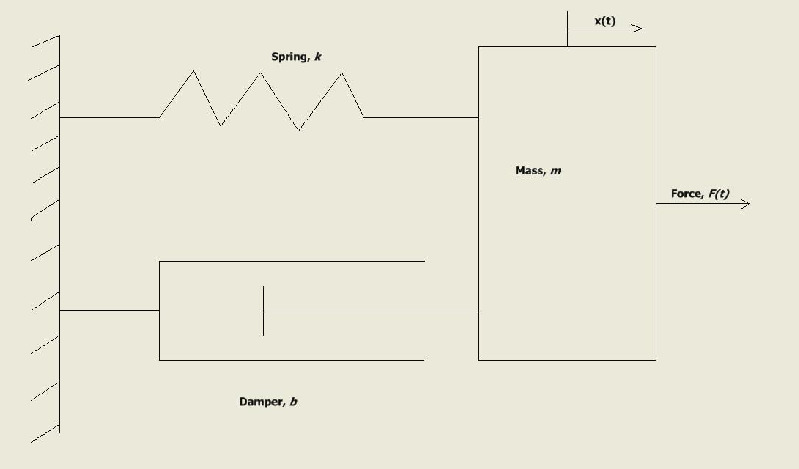
\includegraphics[height=5em,width=10em]{figures/spring-mass-damper.jpg} & 
		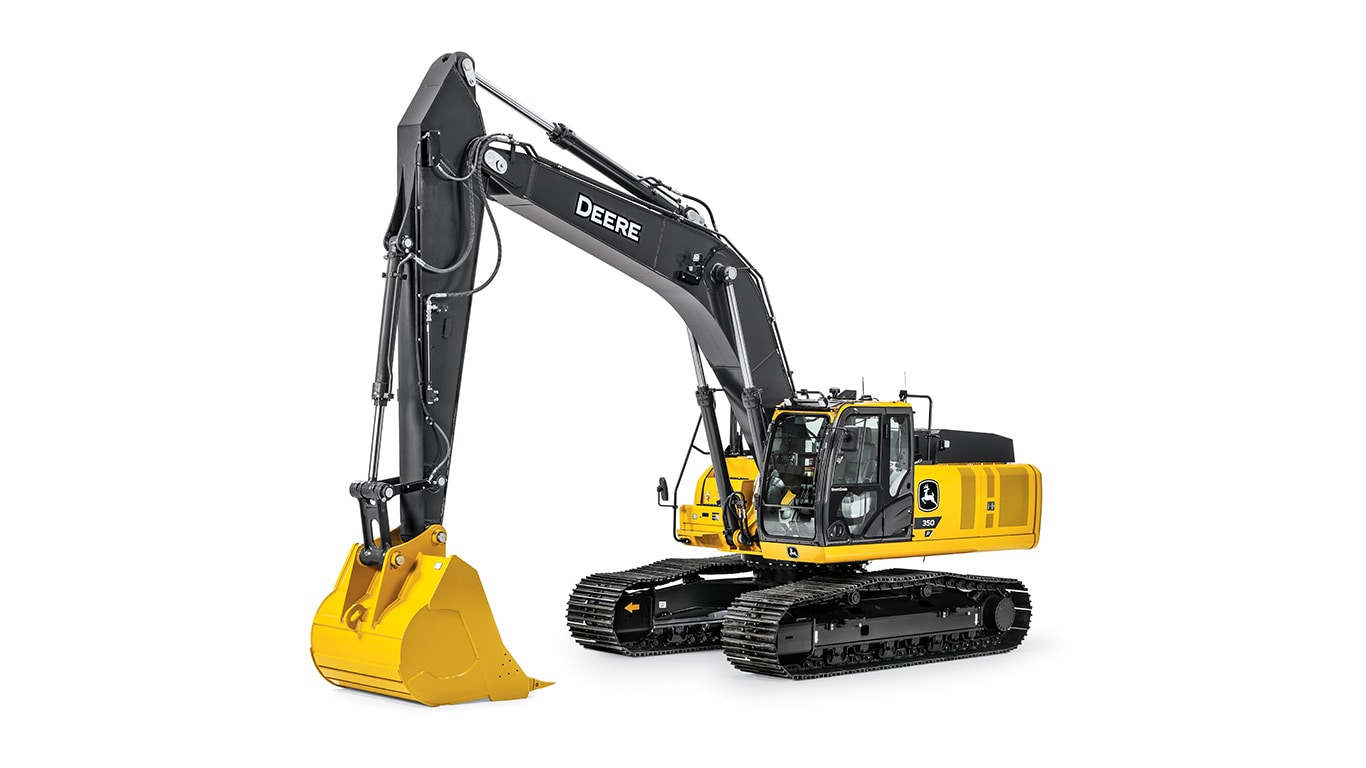
\includegraphics[height=5em,width=10em]{figures/excavJohnDeere.jpg} \\
		\hline \\
		Car suspension & Daimler  Plant \\
		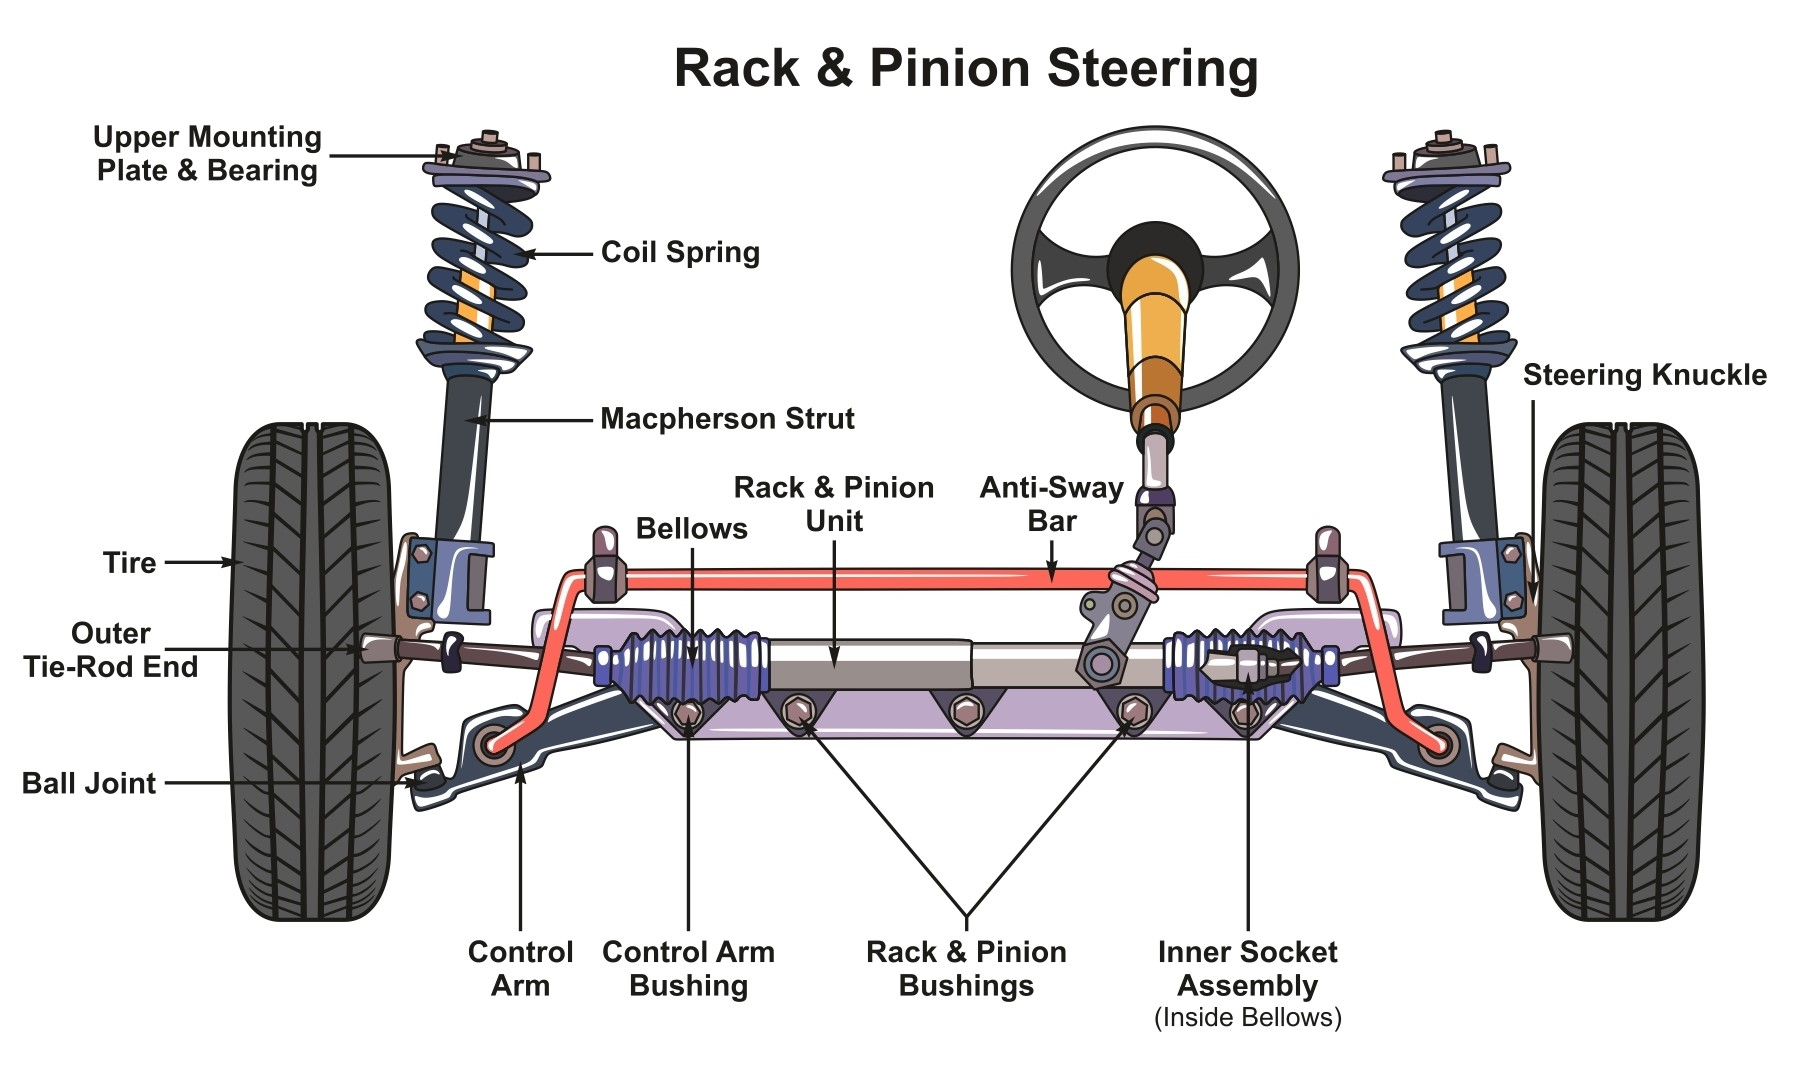
\includegraphics[height=5em,width=10em]{figures/carsusp.jpg} &
		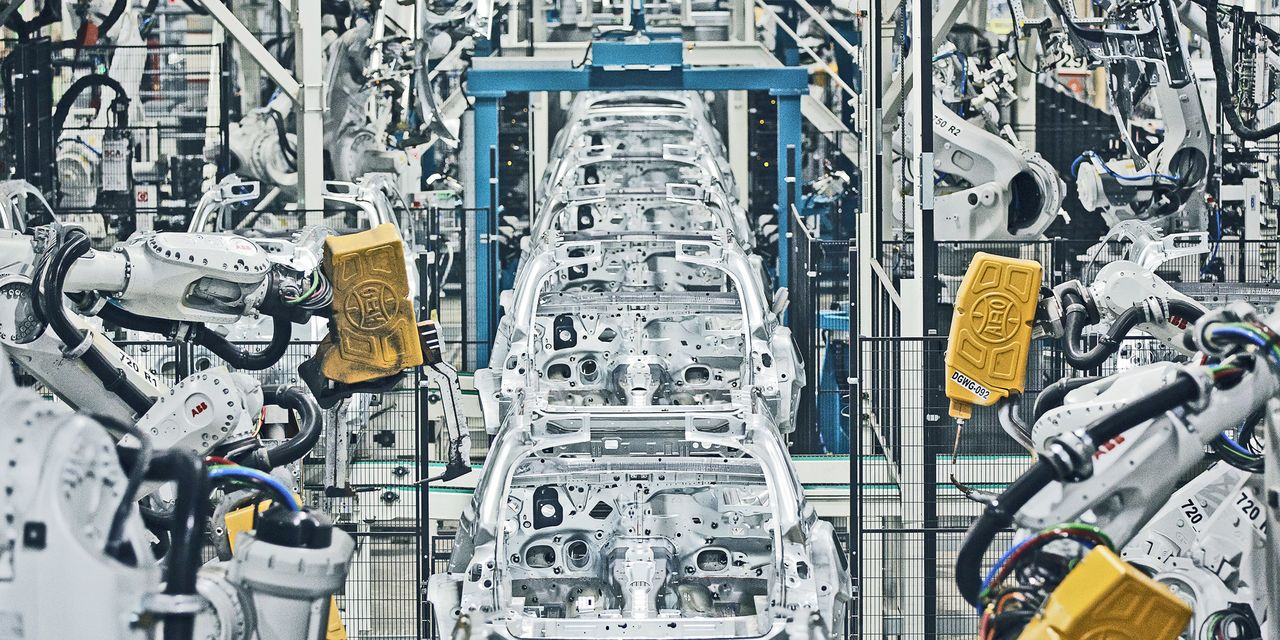
\includegraphics[height=5em,width=10em]{figures/daimler_manuf.jpeg} \\
		\hline
	\end{tabular}
\end{frame}

\subsection{Pairs and Linkages}
\begin{frame}
	\frametitle{Lower Pairs, Higher Pairs, Linkages}
	%
	\begin{block}{Lower and Higher Pairs}
		When elements of pairs touch one another over a \textcolor{red}{substantial region of a surface covering a line, curve-surface, or point of contact}, we have \textcolor{blue}{lower pairs}. When they touch \textcolor{red}{along a discrete line, curve-surface, or point of contact}, we have \textcolor{blue}{higher pairs}.
	\end{block}
	%
	\begin{block}{Linkage (Hunt, 1978)}
		If all joints of a \textcolor{red}{mechanism or mechanical movement} belong to lower pairs, we have a \textcolor{blue}{linkage}. 
	\end{block}
	%
\end{frame}

\begin{frame}
	\frametitle{Prismatic Pairs or $P$-pairs}
	%
	\begin{columns}[t]	
	\begin{column}{.56\textwidth}
		\begin{block}{Hunt, 1978}
		{Formed by receding the axis of the revolution surface between two pairs to $\infty$ so that the \textcolor{blue}{curve} that produces the surface moves parallel to itself, \textcolor{green}{tracing a cylinder}; or a \textcolor{blue}{polygonal-tracing curve} generates a \textcolor{green}{prism}.}
		\end{block}
	\end{column}
		
	\begin{column}{.45\textwidth}
		\begin{figure}
			\centering
			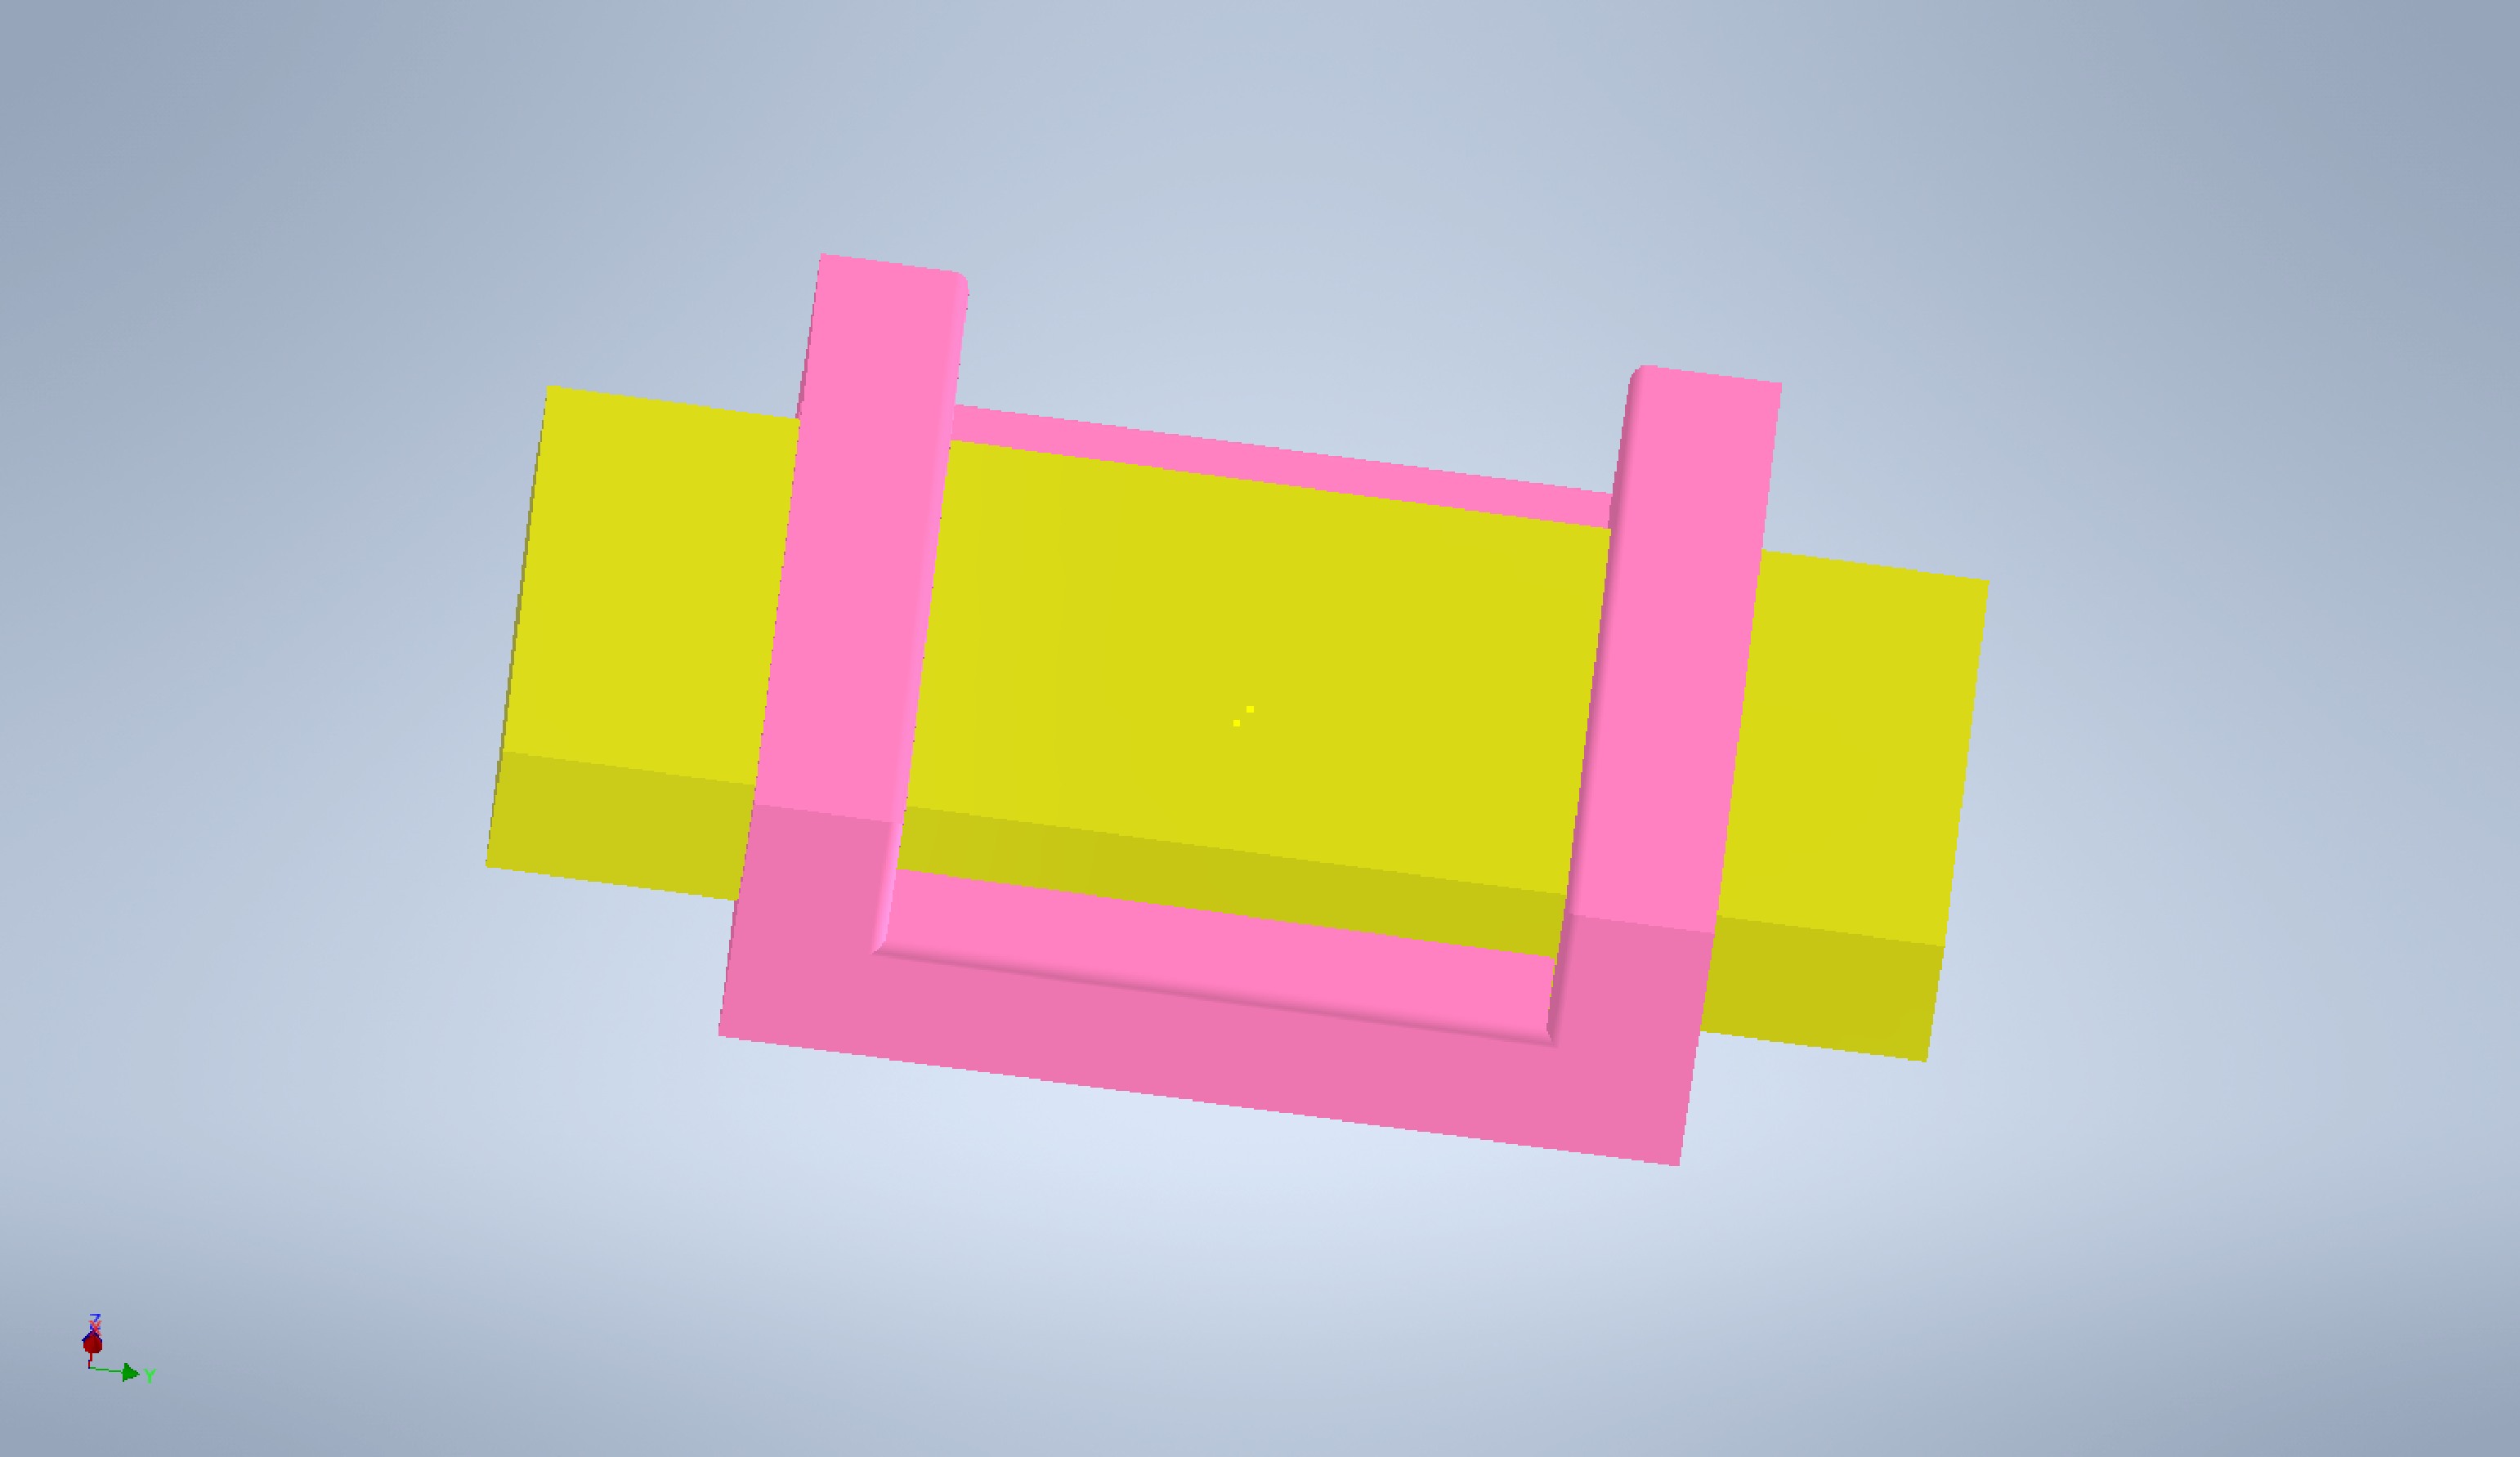
\includegraphics[width=\textwidth]{../Notes/figures/prismatic_joint.pdf}
		\end{figure}
	\end{column}
	\end{columns}
\end{frame}

\begin{frame}
	\frametitle{Revolute Pairs or $R$-pairs}
	%
	\footnotesize{One \textcolor{red}{convex surface} and \textcolor{red}{one non-convex} surface for a \textcolor{green}{one degree of rotational freedom} around the one \textcolor{blue}{joint} the two surfaces make.}
	%\note{An R-pair has a convex and non-convex surface. Revolution surface can be traced by any general curve, outside a planar curve or a circle with axis of revolution about center as it produces an $S$-pair element.}
	\begin{columns}[t]		
		\begin{column}{.5\textwidth}
			\begin{figure}
				\centering
				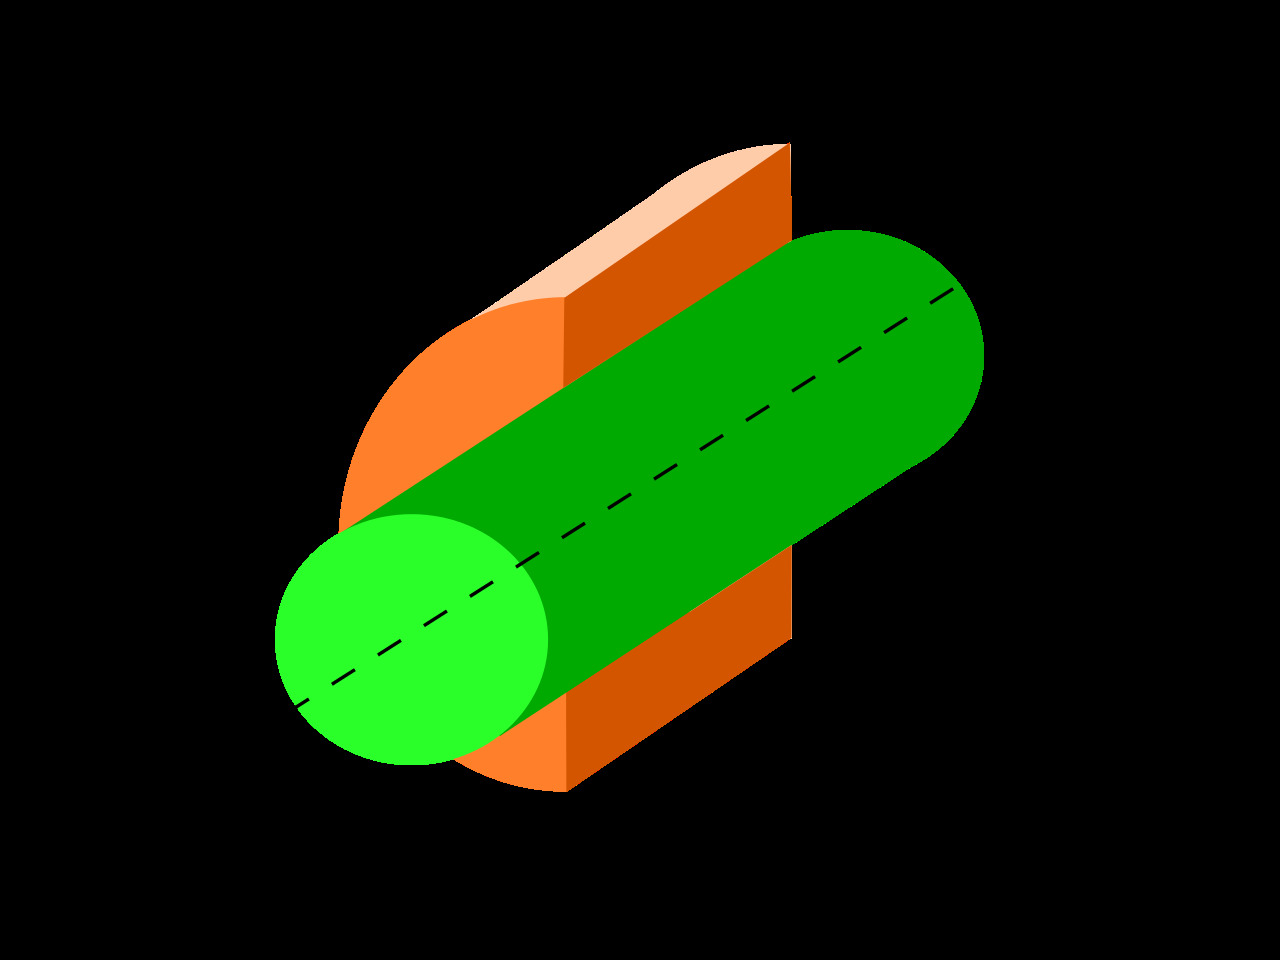
\includegraphics[width=\textwidth]{figures/revolute.jpg}
			\end{figure}
		\end{column}
		\begin{column}{.5\textwidth}
			\begin{figure}
				\centering
				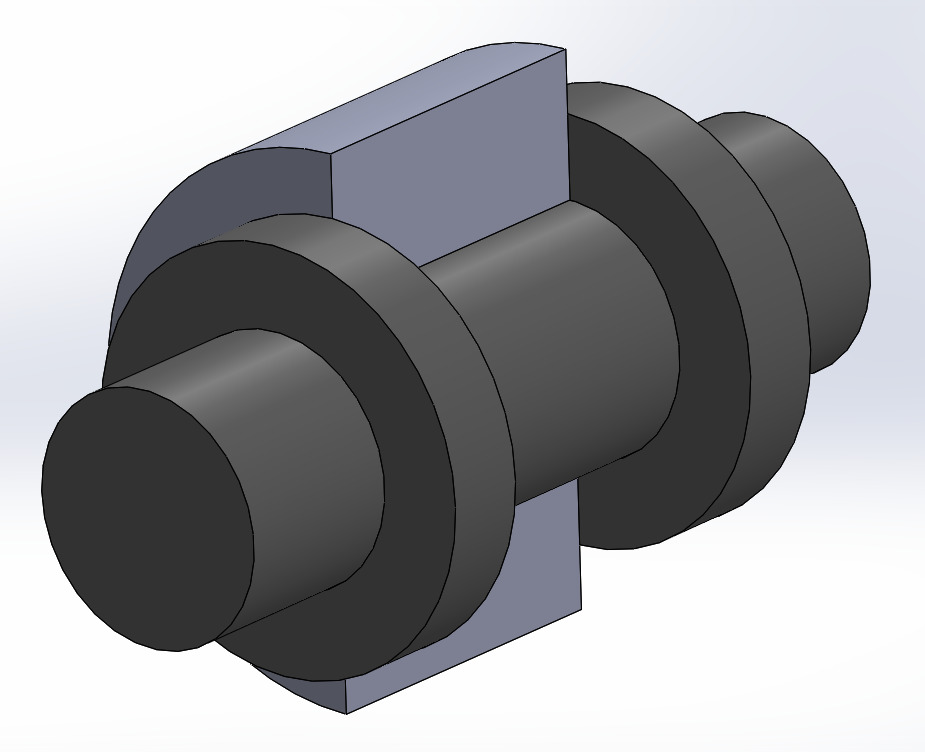
\includegraphics[width=\textwidth]{figures/revolute_cutaway.jpg}
			\end{figure}
		\end{column}
	\end{columns}
	%
	 \footnotesize{\textcolor{red}{Revolute} or \textcolor{red}{Hinge} or \textcolor{red}{Turning} or simply \textcolor{red}{$R$-pairs} with and without shoulder cutaway geometries. Credit: Wikimedia commons.}
\end{frame}


\begin{frame}
	\frametitle{Helical- \& U-Joints}
	%
	\begin{columns}[t]		
		\begin{column}{.5\textwidth}
			\begin{figure}
				\centering
				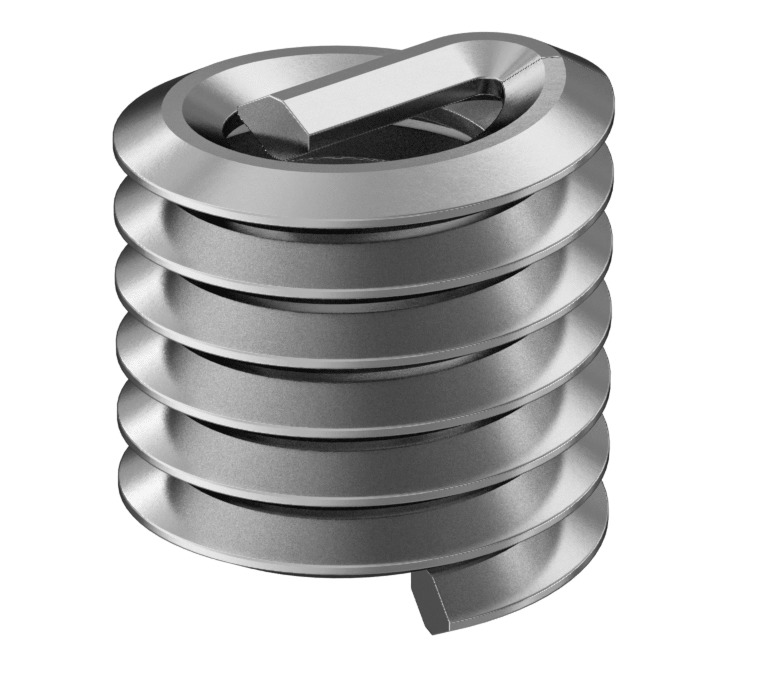
\includegraphics[width=\textwidth]{figures/helical.jpg}
			\end{figure}
			\centering Helical Joint
		\end{column}	
		\begin{column}{.5\textwidth}
			\begin{figure}
			\centering
			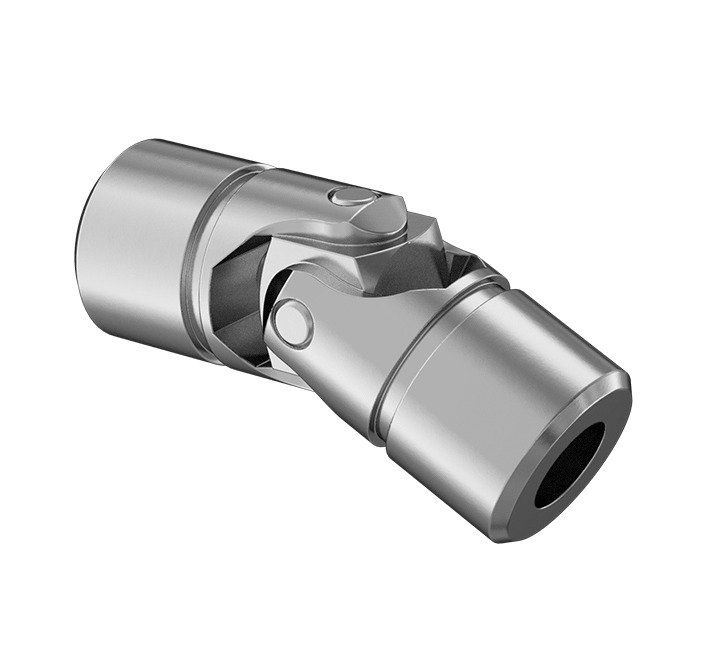
\includegraphics[width=\textwidth]{figures/ujoint.jpg}
			\end{figure}
			\centering Universal Joint
		\end{column}
	\end{columns}
	%
	\footnotesize{\copyright McMaster Carr, May 2022.}
\end{frame}


%\note{Introduce the concept of lower and higher pairs. Then explain a linkage.}



\begin{frame}
	\frametitle{Common Lower Kinematic Pairs}
	%
	\begin{figure}[t]
		\centering
		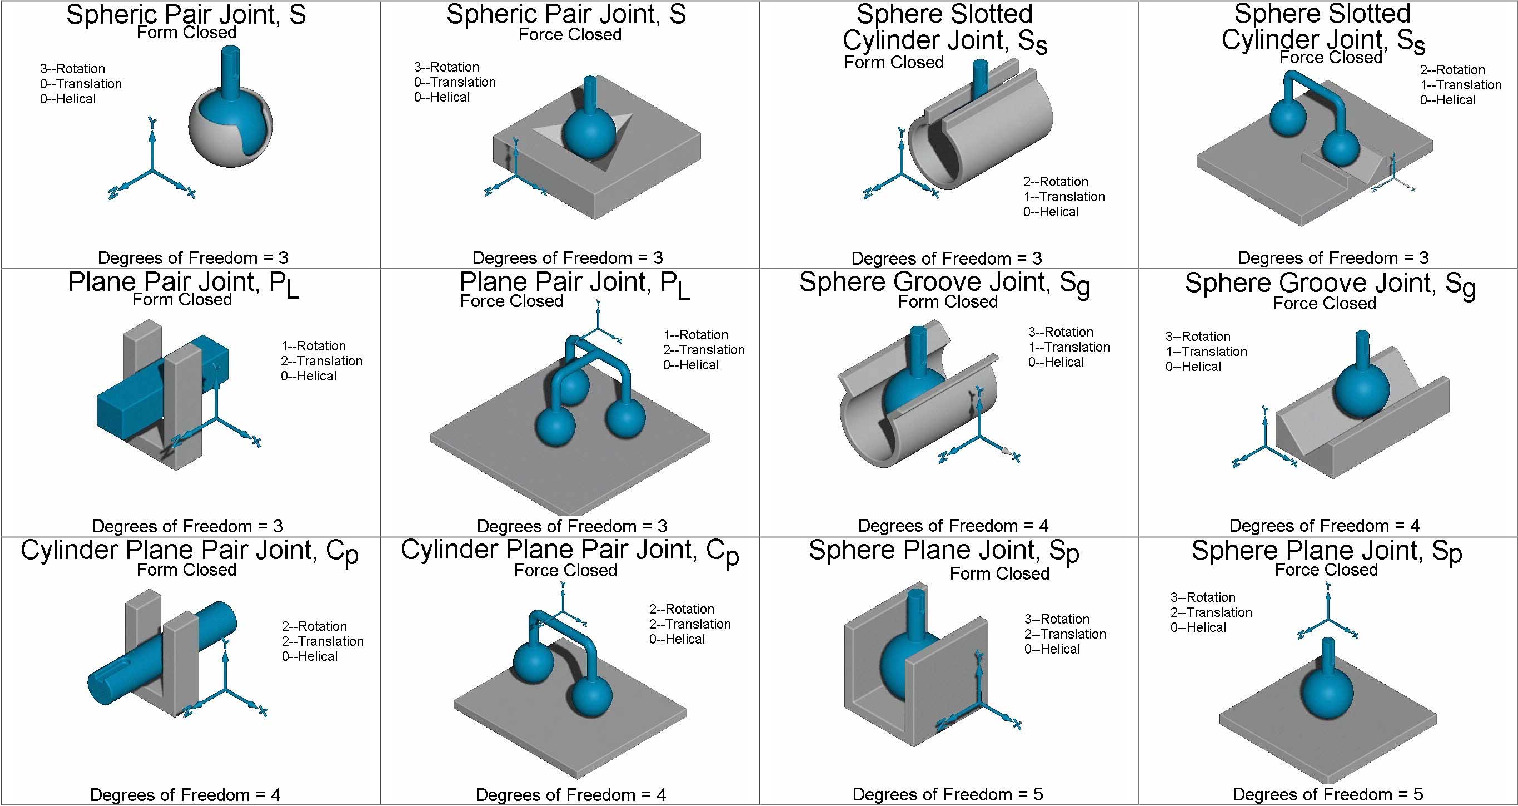
\includegraphics[width=\columnwidth]{figures/pairs2.jpg}
		Credit: \href{https://www.semanticscholar.org/paper/Development-of-Solid-Models-and-Multimedia-of-Pairs-Wharton-Singh/7ba9c2f3cfed5a493bb5828976689764d024b087}{\textcolor{blue}{Wharton and Singh,  2001}}.
	\end{figure}
\end{frame}


\begin{frame}
	\frametitle{Common Lower Kinematic Pairs}
	%
	\begin{figure}[t]
		\centering
		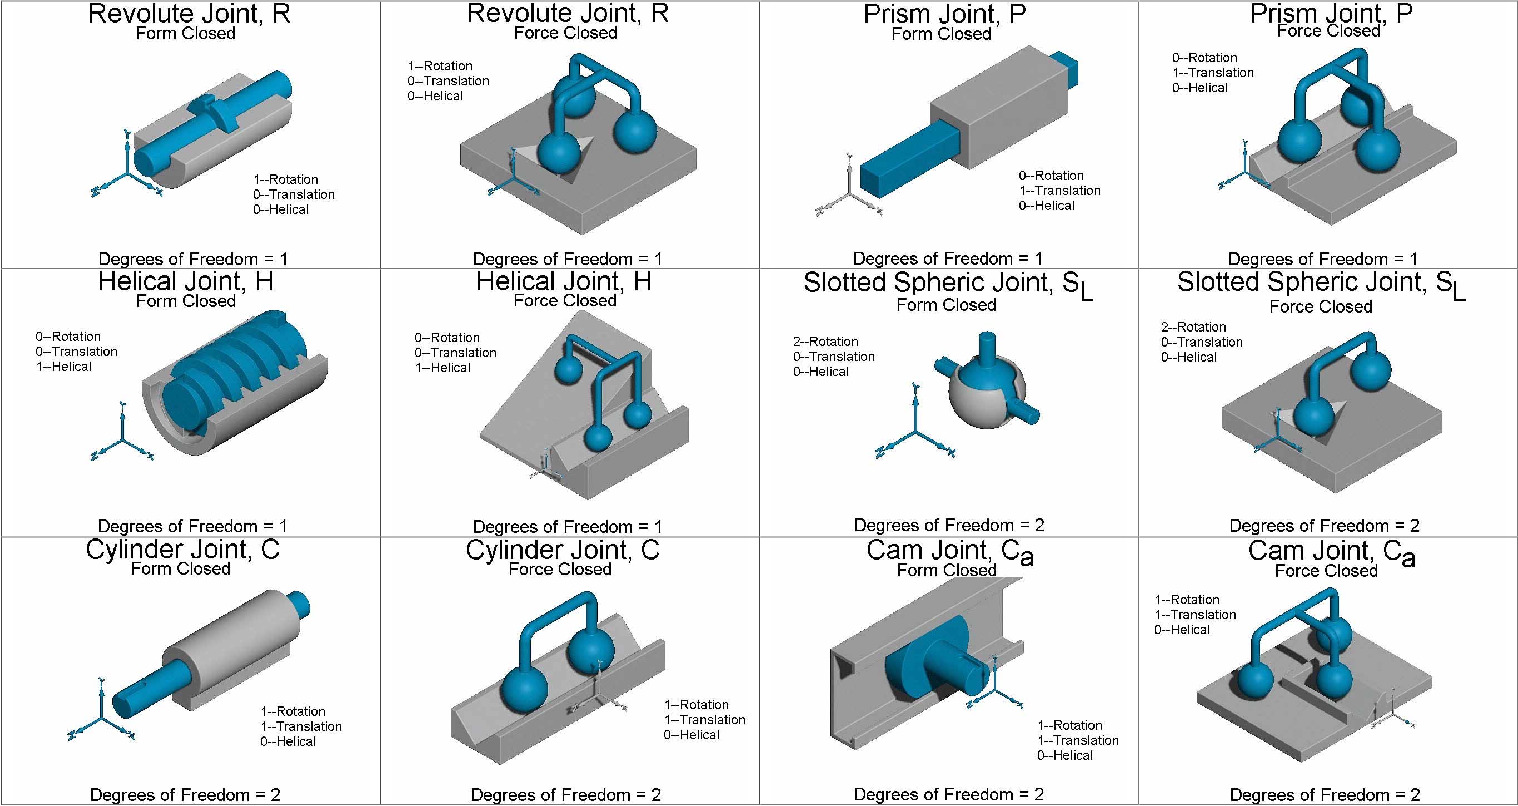
\includegraphics[width=\columnwidth]{figures/pairs.jpg}
		Credit: \href{https://www.semanticscholar.org/paper/Development-of-Solid-Models-and-Multimedia-of-Pairs-Wharton-Singh/7ba9c2f3cfed5a493bb5828976689764d024b087}{\textcolor{blue}{Wharton and Singh,  2001}}.
	\end{figure}
\end{frame}
	
	
\begin{frame}
	\frametitle{Kinematic Geometry of Common Actuations}
	\begin{block}{In-series vs. Parallel-actuated lower pairs}
		\begin{columns}[t]
			\begin{column}{10cm}
				\centering
				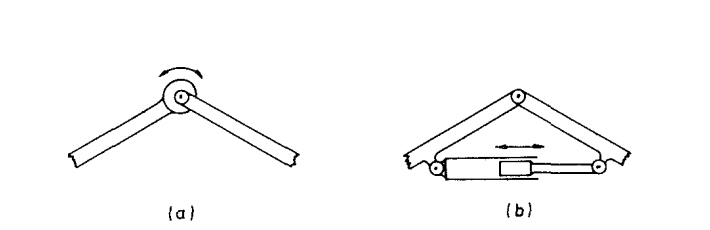
\includegraphics[width=\textwidth]{../Notes/figures/arms_hunt.png}
			\end{column}
		\end{columns}
		\footnotesize{(a): In-series-actuated kinematic pair with a rotary joint that is actuated ``about" the hinge. (b): Prismatic joint actuated ``across" a hinge. Reprinted from Hunt, Kenneth. Structural Kinematics of In-Parallel-Actuated Robot Arms. Transactions of ASME. 1983. }
	\end{block}
\end{frame}
		
\begin{frame}
	\frametitle{Kinematic Chains}
	%	
	\begin{block}{Kinematic Chains (Reuleaux, 1975)}
			We can explain the structural similarity of many mechanisms by parts of \textcolor{red}{kinematic chains} connected by pairs.
	\end{block}
	\begin{block}{Kinematic chains}
		\textcolor{blue}{Kinematic chains} are essentially the basic building structure of \textcolor{red}{mechanisms} $\ldots$ \textcolor{red}{and robots!} 
	\end{block}
\end{frame}
	
%\begin{frame}
%		\frametitle{Kinematic Chains}
%		%\begin{block}{.5\textwidth}
%		\begin{columns}[t]
%			\begin{column}{5cm}
%					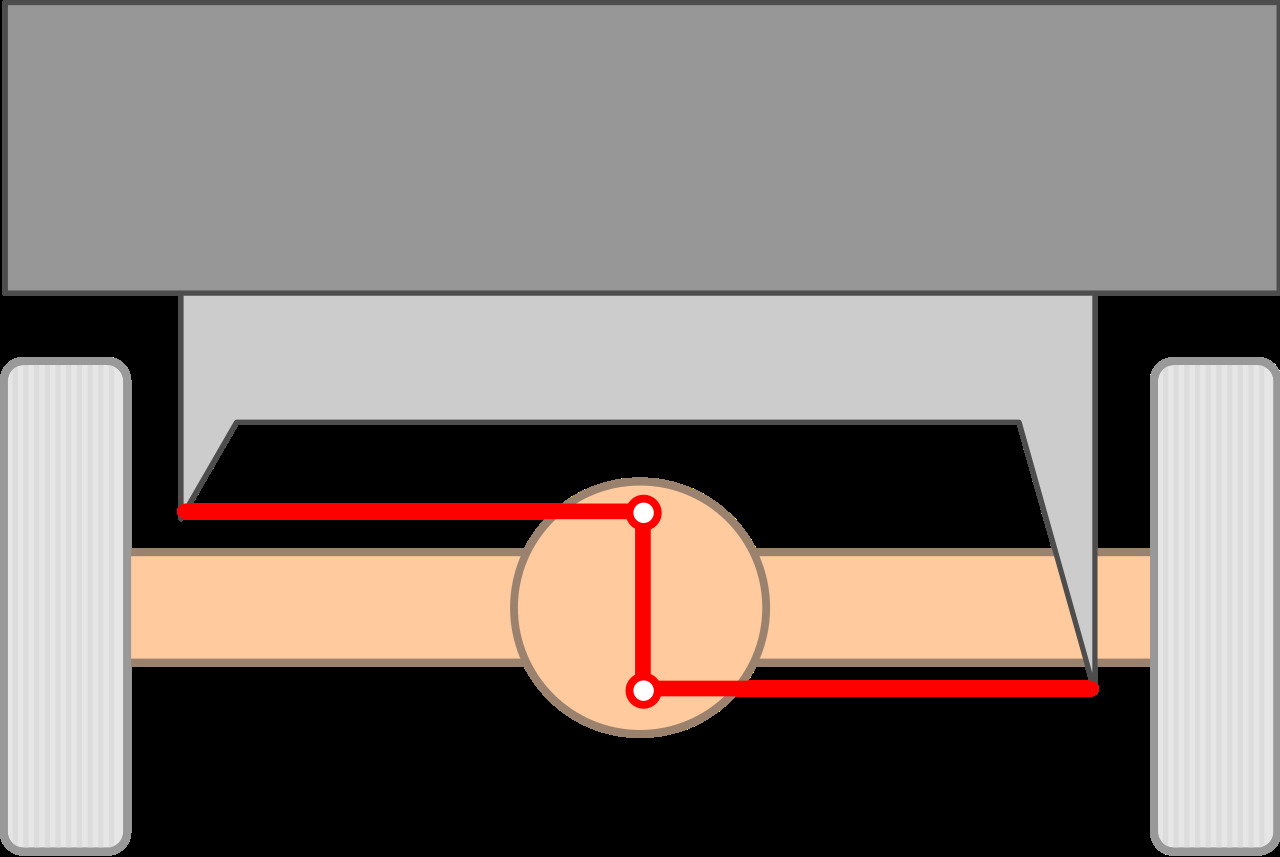
\includegraphics[width=1.5\textwidth, height=1.5\textwidth]{figures/WattsLinkage.jpg} 
%					\footnotesize{The Watt's Linkage Vehicle Suspension.} 
%		\end{column}
%			%	
%		\begin{column}{5cm}
%			\begin{minipage}[b]{.5\textwidth}
%				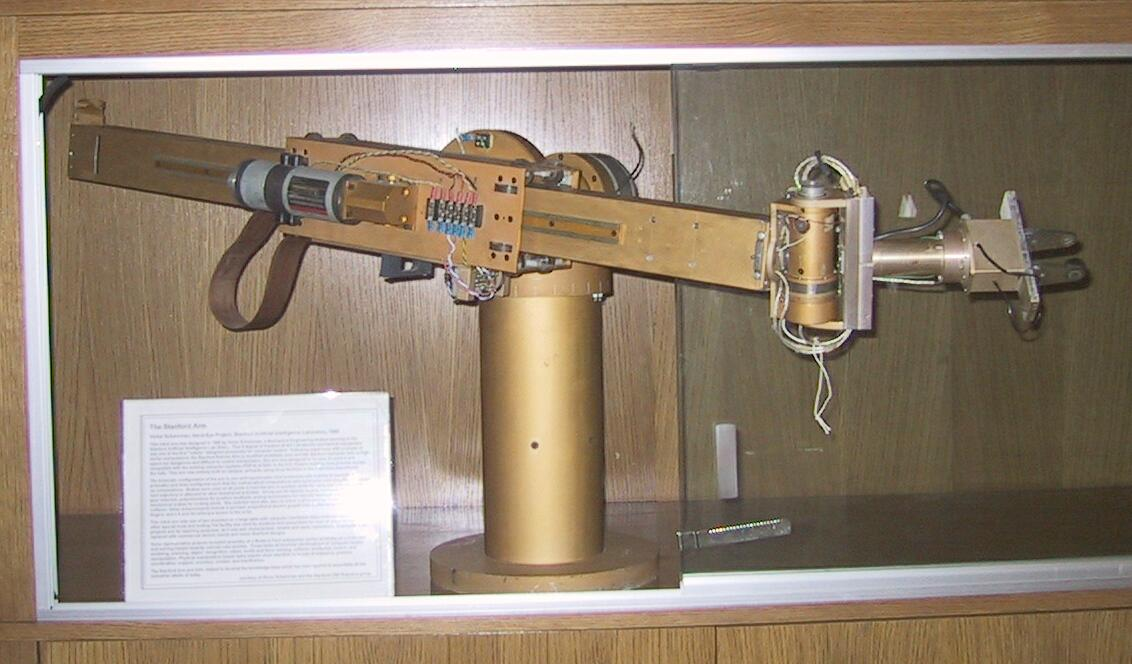
\includegraphics[width=1.5\textwidth, height=1.5\textwidth]{../Notes/figures/StanfordArm.jpg}  \\
%				\footnotesize The Stanford Arm (Infolab 1969). %Six degrees of freedom open kinematic chain.
%			\end{minipage}
%		\end{column}
%	\end{columns}
%%\end{block}
%\end{frame}

\subsection{Serial Chains}
	\begin{frame}
		\frametitle{Open Kinematic Chains}
		%	
		\begin{block}{Chains}
			Open kinematic chains are based off the anthropomorphic construction of the human hand with cantilevered beam structures.
		\end{block}
		\begin{block}{Chain Mechanisms and Error Amplification}
			Amplifies errors from waist (or base frame) all the way to the tool frame. Control difficult. 
		\end{block}
		%
		\begin{block}{Control}
			Feedforward control: High power and precision hydraulic actuators for servo motors. \\
			Sensory feedback control: Force sensing (Ernst, 1962). 
		\end{block}
	\end{frame}
	
	
	\note{The PUMA arm is the world's first serial kinematic chain. Developer: Victor Scheinman, Stanford student in the `50's. Made several iterations. Patent Rights: Joe Engelberger, (Danbury Unimation, 1961). Joe -- father of robotics -- created world's first robotics company in '61.}
	\begin{frame}
		\frametitle{Open Kinematic Lower Pairs}
		\begin{definition}[Ken Salisbury Jr., 1982]
			``\footnotesize \textit{[Robots are] our fascination with constructing mechanical analogues of ourselves... [this fascination] has led us to place all sorts of hopes and expectations in robot capabilities}."
		\end{definition}
		\begin{columns}[t]
			\begin{column}{5cm}
				\begin{minipage}[b]{.5\textwidth}
					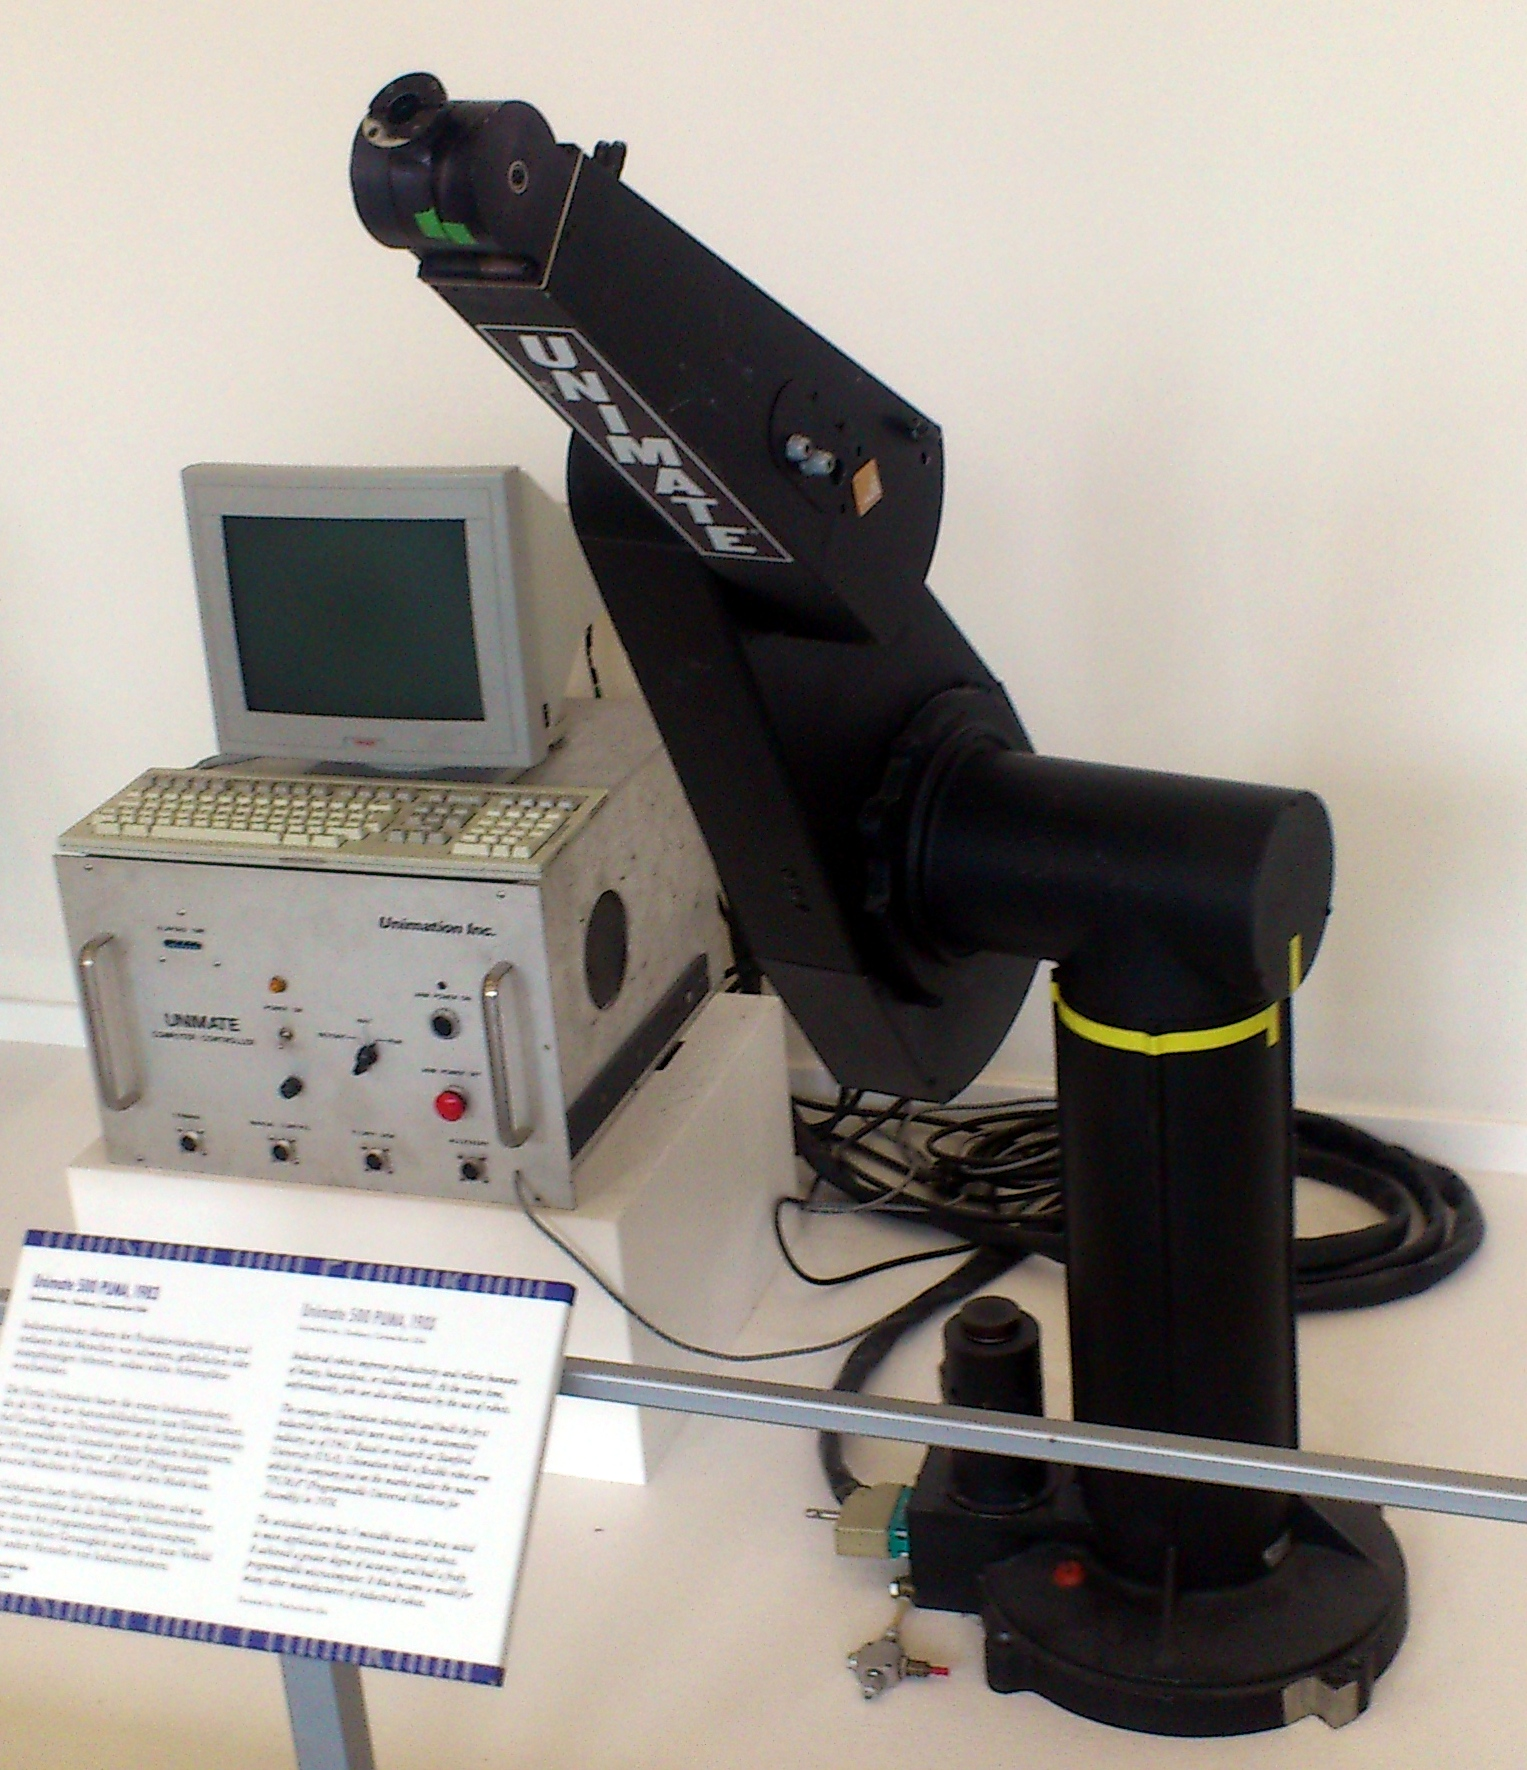
\includegraphics[width=1.5\textwidth, height=1.5\textwidth]{../Notes/figures/PUMA.jpg} \\
					\footnotesize{The PUMA Robot (1956).} %Programmable Universal Manipulation Arm.}
			\end{minipage}
			%
		\end{column}	
		\begin{column}{5cm}
			\begin{minipage}[b]{.5\textwidth}
				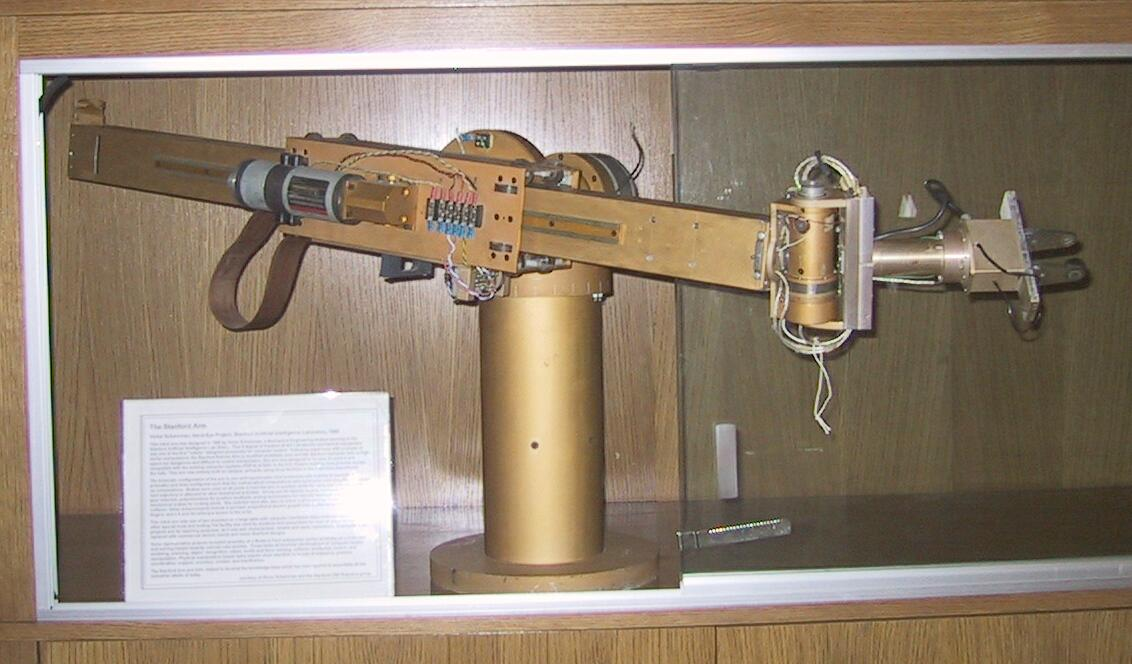
\includegraphics[width=1.5\textwidth, height=1.5\textwidth]{../Notes/figures/StanfordArm.jpg}  \\
				\footnotesize The Stanford Arm (Infolab 1969). %Six degrees of freedom open kinematic chain.
			\end{minipage}
		\end{column}
	\end{columns}
\end{frame}


\begin{frame}
\frametitle{Open Kinematic Chains}
%
\begin{tcolorbox}[coltitle=blue!80!yellow,colframe=brown!80]
	Open kinematic chains provide unstructured environmental interaction.
\end{tcolorbox}
\begin{tcolorbox}[coltitle=blue!80!yellow,colframe=gray!100]
	Project MAC, MIT.
\end{tcolorbox}
\begin{tcolorbox}[coltitle=blue!80!yellow,colframe=black!80]
	Tomovic and Boni's pressure sensed grasp.
\end{tcolorbox}
\begin{tcolorbox}[coltitle=blue!80!yellow,colframe=pink!100]
	Binary robot vision system (McCarthy et al, 1963).
\end{tcolorbox}
\end{frame}

\begin{frame}
\frametitle{Open Kinematic Chains}
%
\begin{tcolorbox}[coltitle=cyan!80,colframe=green!100]
	Stanford Manipulator.
\end{tcolorbox}
\begin{tcolorbox}[coltitle=blue!80!yellow,colframe=blue!100]
	Boston arm.
\end{tcolorbox}
\begin{tcolorbox}[coltitle=blue!80!yellow,colframe=red!100]
	The AMF (American Machines and Foundry) arm.
\end{tcolorbox}
\begin{tcolorbox}[coltitle=blue!80!yellow,colframe=yellow!100]
	General electric's walking robot (1969).
\end{tcolorbox}
\end{frame}


\begin{frame}
\frametitle{Long Walk Towards Direct Drive Robot Arms}

\begin{tcolorbox}[coltitle=magenta!80!green,colframe=yellow!80!green]
	The 50's, 60's nd 70's witnessed use of hydraulics  for (feedforward) position control.
\end{tcolorbox}

\begin{tcolorbox}[coltitle=magenta!80!green,colframe=blue!80!green] 
	For feedback control, force sensors and pressure sensors were used in closed-loop scenarios.
\end{tcolorbox}

\begin{tcolorbox}[coltitle=magenta!80!green,colframe=red!80!green] 
	Electrical actuation meant that robots had to be operated at high speeds. Needs for gear reduction for safe operations at low speeds. 
\end{tcolorbox}

\begin{tcolorbox}[coltitle=magenta!80!green,colframe=brown!80!green]
	With gear reduction came backlash, friction, and associated expenses.
\end{tcolorbox}
\end{frame}


\note{CMU DD I/II Arms: Workspace is donut shaped. OD:  90cm; ID: 21.7cm; $1.8m^2$ workspace area. Built by Harry Asada. Structural design similar to aircraft gimbal arm; Uses Samarium Cobalt rare earth magnet brushless DC motors on first 3 joints, and AlNiCo magnets on tip joints. No belts, transmissions making for faster transmitting of motions, less friction, low energy, low compliance. Each joint has complex AL housing which enables: (i) Control of geometrical relationships of bearing assembly; (ii) Control of servo components to bearing assembly; (iii) Controls of rotational axes to consecutive joints.}


\begin{frame}
\frametitle{Direct Drive Robot Mechanism: CMU DD I Arm}
\begin{tcolorbox}[coltitle=blue!80!yellow,colframe=brown!80!green]
	Along came Harry Asada.
\end{tcolorbox}
\begin{columns}[t]	
	%
	\begin{column}{.45\columnwidth}
		\begin{minipage}[b]{\textwidth}
			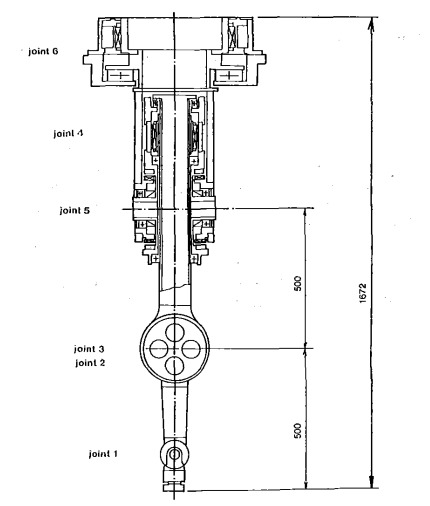
\includegraphics[width=1.2\textwidth, height=1.2\textwidth]{figures/cmu_arm.jpg} \\
			\footnotesize{Arm Schematics Transmission} %Programmable Universal Manipulation Arm.}
	\end{minipage}
	%
\end{column}
%
\begin{column}{.45\columnwidth}
	\begin{minipage}[b]{\textwidth}
		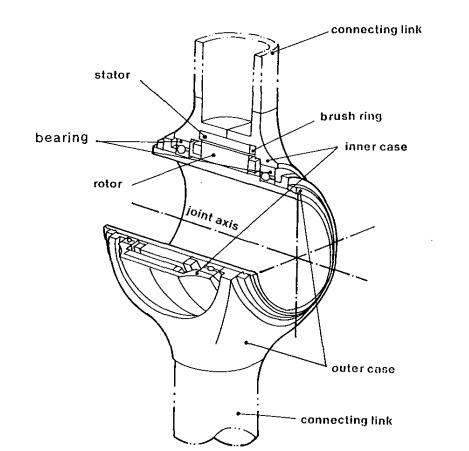
\includegraphics[width=1.2\textwidth, height=1.2\textwidth]{figures/dd_joints.jpg} \\
		\footnotesize{Joint schematic} %Programmable Universal Manipulation Arm.}
\end{minipage}
%
\end{column}
\end{columns}
\end{frame}

\begin{frame}
\frametitle{Direct Drive Robot Mechanism: CMU DD I Arm}
\begin{columns}[t]					%
%
\begin{column}{.45\columnwidth}
\begin{minipage}[b]{\textwidth}
	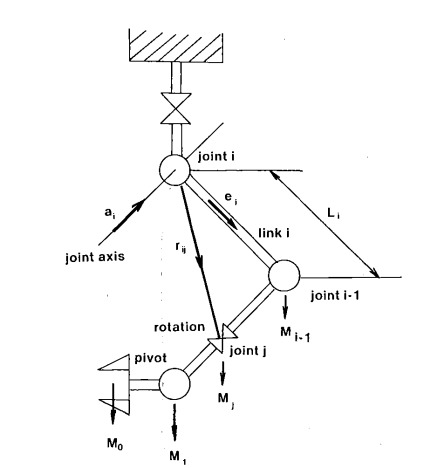
\includegraphics[width=1.1\textwidth, height=1.5\textwidth]{figures/dd_kinematics.jpg} \\
	\footnotesize{Kinematic model} %Programmable Universal Manipulation Arm.}
\end{minipage}
%
\end{column}
\begin{column}{.45\columnwidth}
\begin{minipage}[b]{\textwidth}
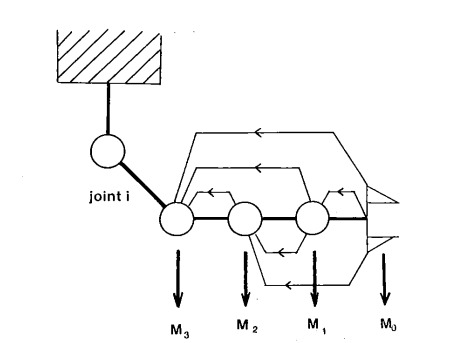
\includegraphics[width=1.2\textwidth, height=1.5\textwidth]{figures/dd_load_joints.jpg} \\
\footnotesize{Errors Transmission} %Programmable Universal Manipulation Arm.}
\end{minipage}
\end{column}
\end{columns}\end{frame}


\note{First direct-drive robot without a gearbox. Selective compliance in X-Y directions given its articulated jointed arms. One-freedom motion along $Z$ direction given its constrained arm New generations such as Cobra i600/i800 include power amplifiers, system and servo controls etc embedded in the robot's base. Kuka Scara arm: Lightweight, fast, powerful, low maintenance, energy consumption, investment costs etc.}
\begin{frame}
\frametitle{SCARA Robot Mechanisms}
\begin{columns}[t]	
\begin{column}{5cm}
\begin{minipage}[b]{.5\textwidth}
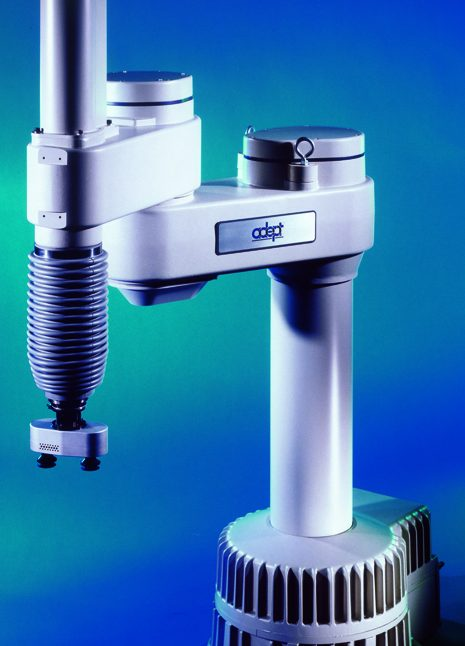
\includegraphics[width=1.5\textwidth, height=1.5\textwidth]{figures/adeptone.jpg}  \\
\footnotesize The Adept One SCARA robot (Debuted 1984). 
\end{minipage}
\end{column}
%
\begin{column}{5cm}
\begin{minipage}[b]{.5\textwidth}
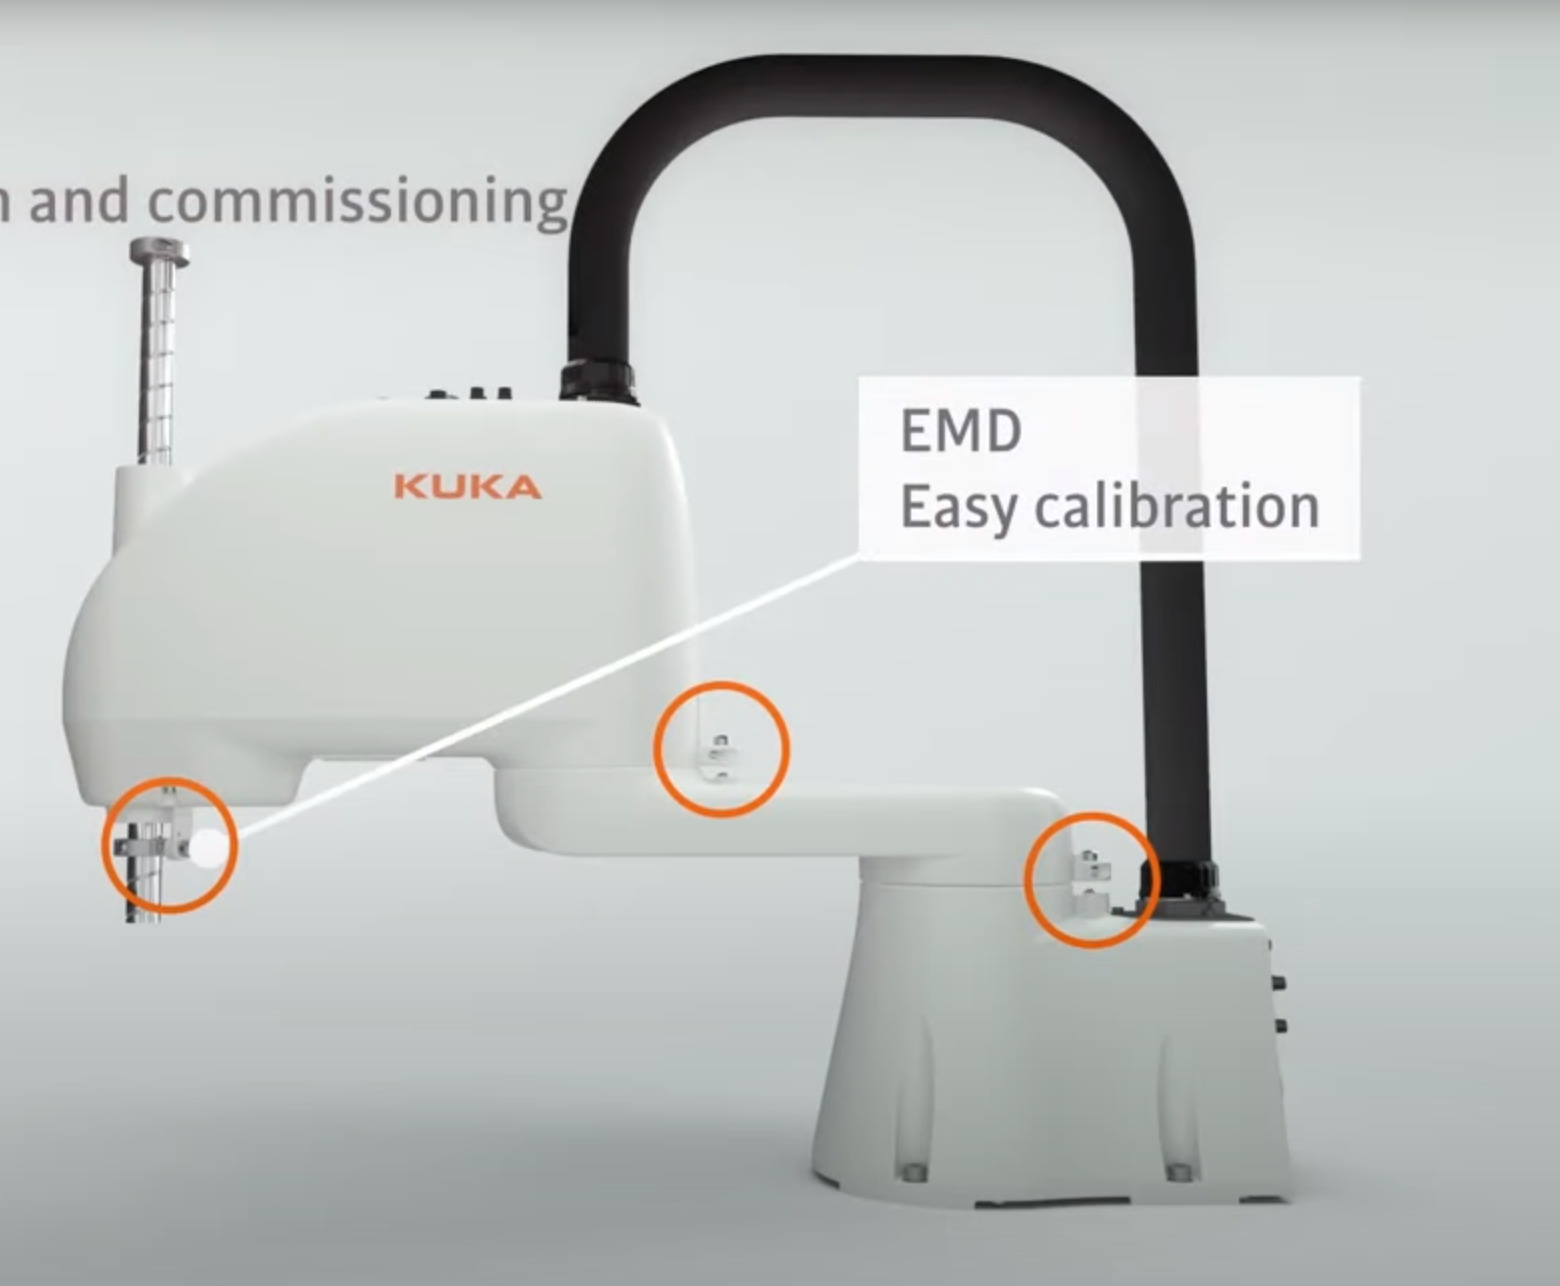
\includegraphics[width=1.5\textwidth, height=1.5\textwidth]{figures/Scara.jpg} \\
\footnotesize{Kuka's SCARA arm, 2022. \copyright Kuka Robotics} %Programmable Universal Manipulation Arm.}
\end{minipage}
%
\end{column}
\end{columns}
\end{frame}


\begin{frame}
	\begin{block}{The St{\"a}ubli anthropomorphic arm.}
		\begin{columns}[t]
			\begin{column}{10cm}
				\centering
				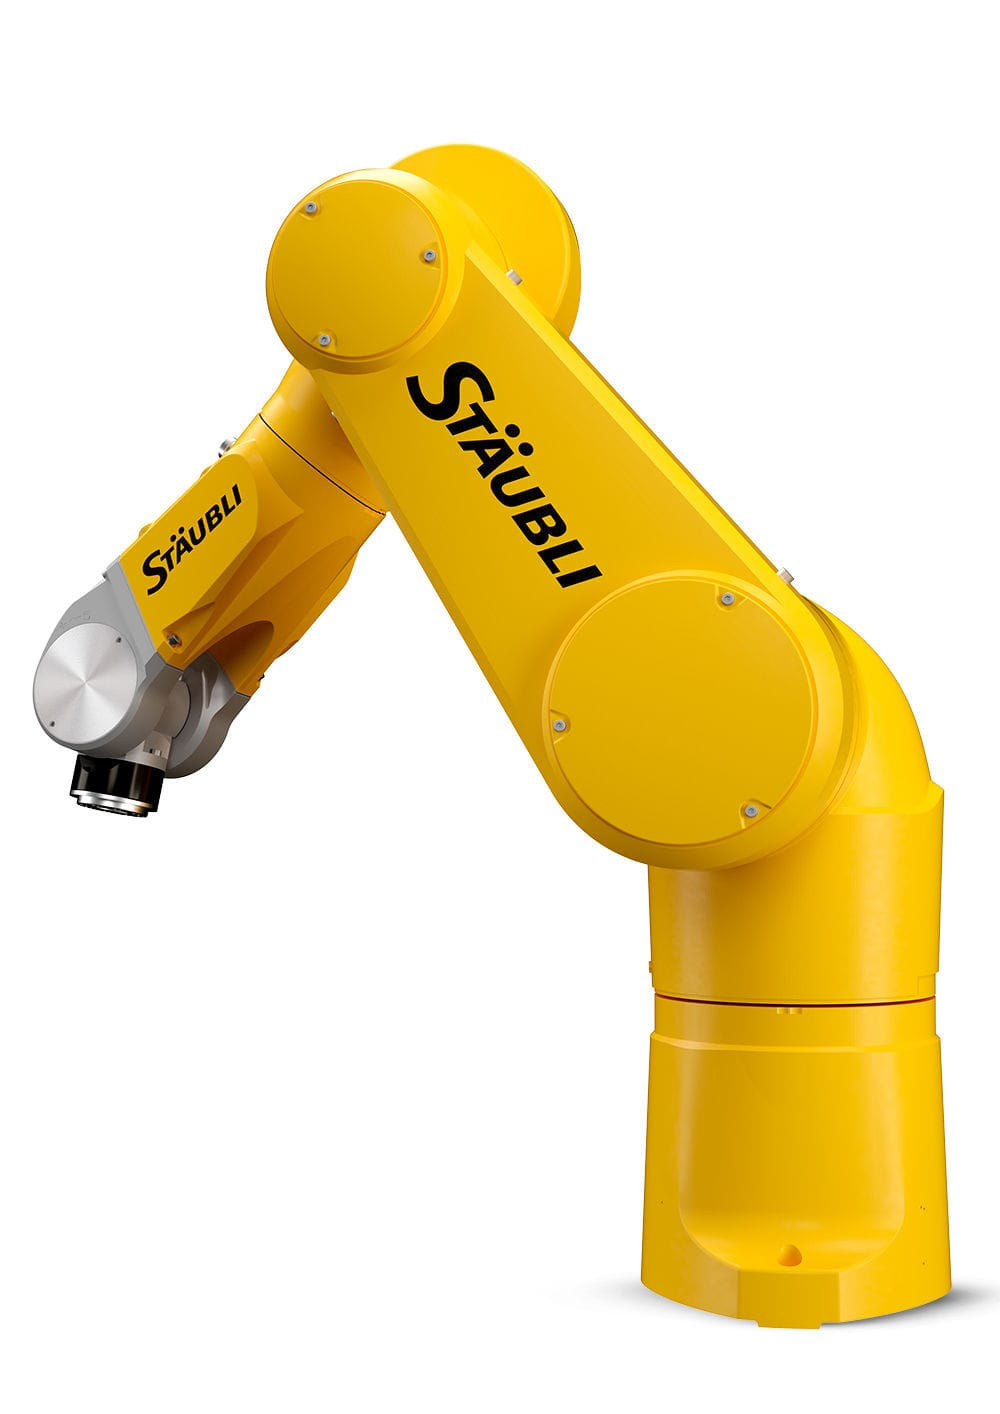
\includegraphics[scale=.1, width=.5\textwidth, rotate=0]{../Notes/figures/Staubli.jpg}
			\end{column}
		\end{columns}
		\footnotesize{The Staubli 6-DOF Arm is an example of a Spherical Manipulator. Reprinted from DirectIndustry's Webpage.}
	\end{block}
\end{frame}

\begin{frame}
\frametitle{Serial mechanisms research in the 80's}
%
\tcbset{coltitle=cyan!80,colframe=gray!80!green,title=Mechanisms in the 80's,
enlarge left by=-5mm,enlarge right by=0mm,width=\linewidth+5mm}
\begin{tcolorbox}[toggle enlargement=none]
With the 80's came the arrival of PCs. Lots of research went into computational algorithms for the kinematics and kinetics of (mostly) anthropomorphic robot arms.
\end{tcolorbox}
\begin{tcolorbox}[coltitle=magenta!70,colframe=blue!80!red,title=Active control schemes,toggle enlargement=forced]
Efficient recursive Lagrangian and computational methods for the gravitational and Coriolis forces in Newton-Euler equations.
\end{tcolorbox}
\end{frame}

\begin{frame}
	\frametitle{Serial mechanisms research in the 80's}
	%
	\tcbset{coltitle=cyan!80,colframe=gray!80!green,title=Mechanisms in the 80's,
		enlarge left by=-5mm,enlarge right by=0mm,width=\linewidth+5mm}
	\begin{tcolorbox}[coltitle=pink!70,colframe=gray!80!red,title=Feedback Linearization,toggle enlargement=evenpage]
		Dynamics feedback linearization for precise bounds on manipulator performance.
	\end{tcolorbox}
	
	\begin{tcolorbox}[title=Automatix,toggle enlargement=none]
		Reconfigurable robots for various assembly ops.
	\end{tcolorbox}
\end{frame}

\begin{frame}
\frametitle{Serial mechanisms research in the 90's}
%
\tcbset{coltitle=pink!80,colframe=gray!80,title=Robotworld,
enlarge left by=-5mm,enlarge right by=0mm,width=\linewidth+5mm}
\begin{columns}[b]
\begin{column}{.48\columnwidth}			
\begin{tcolorbox}[colframe=blue!80!green, coltitle=white!80,toggle enlargement=none]
First industrial-scale re-configurable robot and with machine vision components. RAIL scripting OS originally based on Motorola 68000, later on replaced by Apple Macintosh II. 
\end{tcolorbox}
\end{column}
\begin{column}{.52\columnwidth}
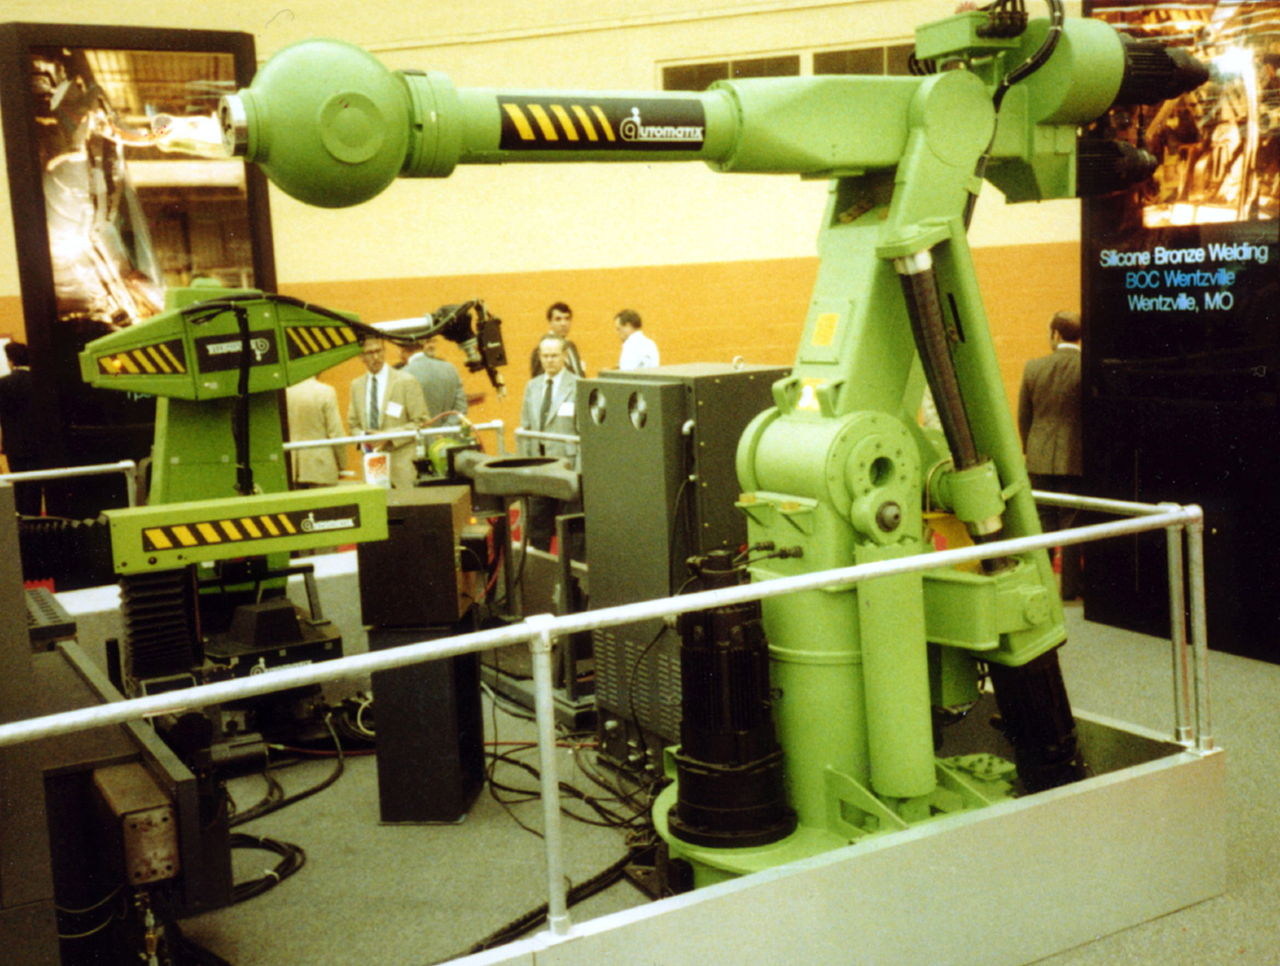
\includegraphics[width=\textwidth]{figures/Automatix.jpg}
\copyright Wikipedia
\end{column}
\end{columns}
\end{frame}

\subsection{Hyperredundant and Parallel robots}
	\begin{frame}
		\frametitle{Hyper-redundant Continuum Robots}
		\begin{columns}[b]
			\begin{column}{.33\columnwidth}			
				\begin{tcolorbox}[colframe=blue!80!green, coltitle=white!80,toggle enlargement=none]
					\centering 
					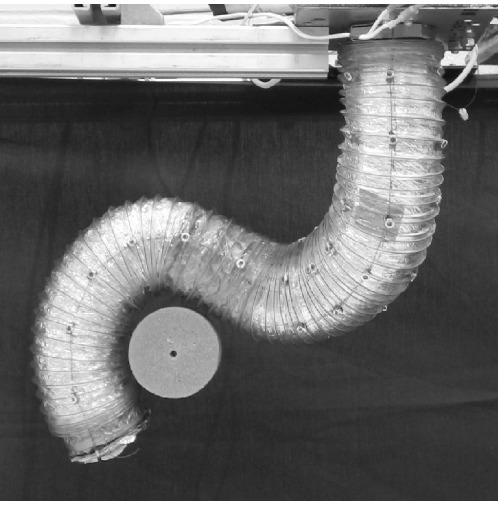
\includegraphics[width=\textwidth, height=1.1\textwidth]{figures/multisec_continuum.jpg}
				\end{tcolorbox}
			\end{column}	
		\begin{column}{.33\columnwidth}			
			\begin{tcolorbox}[colframe=blue!80!green, coltitle=white!80,toggle enlargement=none]
			\centering 
			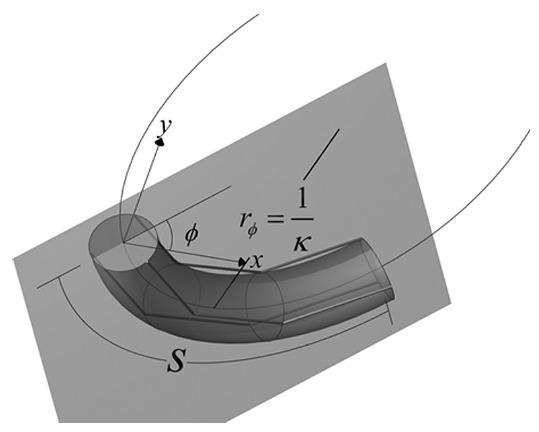
\includegraphics[width=\textwidth, height=1.1\textwidth]{figures/multi_sec_manip.jpg}
			\end{tcolorbox}
		\end{column}	
		\begin{column}{.33\columnwidth}			
			\begin{tcolorbox}[colframe=blue!80!green, coltitle=white!80,toggle enlargement=none]
			\centering 
			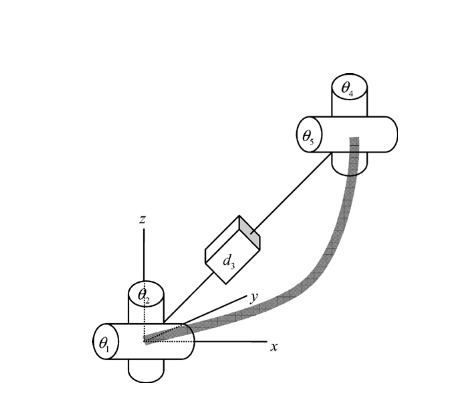
\includegraphics[width=\textwidth, height=1.1\textwidth]{figures/multi_sec_scheme.jpg}
			\end{tcolorbox}
		\end{column}	
		\end{columns}
		\centering \footnotesize{The elephant trunk continuum robot. Jones \& Walker, T-RO 2006. Inspiration: Muscular hydrostats in nature.}
	\end{frame}

\begin{frame}
	\frametitle{Hyper-redundant Kinematic Chains}
	\begin{columns}[b]
		\begin{column}{.98\columnwidth}			
			\begin{tcolorbox}[colframe=blue!80!green, coltitle=white!80,toggle enlargement=none]
				\centering 
				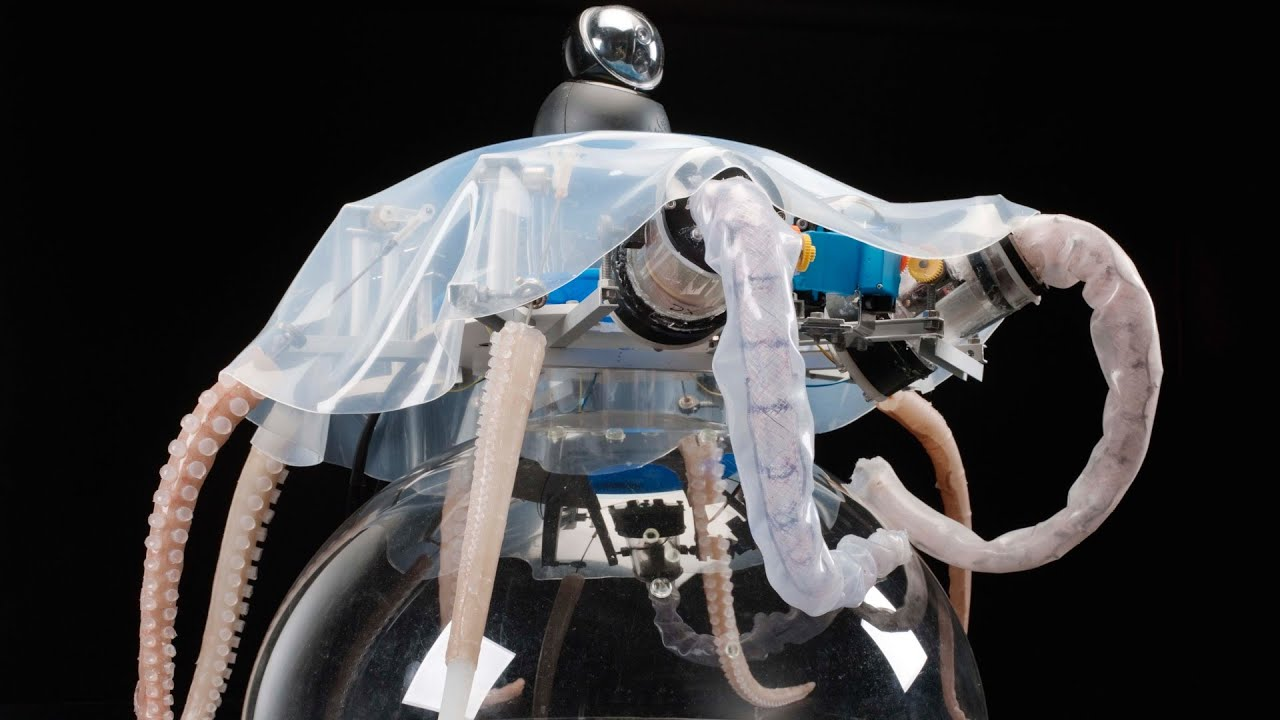
\includegraphics[width=\textwidth]{../Notes/figures/octopus.jpg}
			\end{tcolorbox}
		\end{column}	
	\end{columns}
	 \centering \footnotesize{An octopus-inspired soft robot. \copyright Cecilia Laschi.}
\end{frame}
	
	
	\begin{frame}
		\frametitle{Parallel Robots}
		%
		\tcbset{coltitle=light-blue!100,colframe=cyan!50,title=Robotworld,
			enlarge left by=-5mm,enlarge right by=0mm,width=\linewidth+5mm}
		\begin{tcolorbox}[title=Mehlet 2015,toggle enlargement=none]
			A \textcolor{blue}{parallel robot} is made up of an end-effector with $n$ degrees of freedom, and of a fixed base, linked together by at least two independent kinematic chains. Actuation takes place through n simple actuators.
		\end{tcolorbox}	
	\end{frame}
	
	\begin{frame}
		\frametitle{Parallel mechanisms: Stewart-Gough Platforms}
		\footnotesize{Principles of a moving platform to test tyre wear and tear (Gough, 1947). Prototype, 1955.}
		\newline
		\begin{columns}[b]
			\begin{column}{.48\columnwidth}			
				\begin{tcolorbox}[colframe=blue!80!green, coltitle=white!80,toggle enlargement=none]
					\centering 
					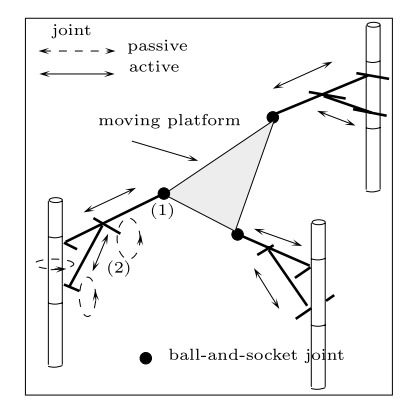
\includegraphics[width=\textwidth]{figures/Stewart.jpg}
				\end{tcolorbox}
			\end{column}
			\begin{column}{.48\columnwidth}			
				\begin{tcolorbox}[colframe=blue!80!green, 	coltitle=white!80,toggle enlargement=none]
				\centering 
				\includegraphics[width=.8\textwidth]{../../../Papers/PhDThesis/figures/GoughPlatform.jpg}
				\end{tcolorbox}
			\end{column}	
		\end{columns}
		\centering \footnotesize{\textit{Left}: Stewart's 1965 mechanism. \textit{Right:} The original 1954 octahedral hexapod proposed by  Gough. Courtesy: Parallemic.org.}
	\end{frame}

\begin{frame}
	\frametitle{Truss Robots}
	\begin{columns}[b]
		\begin{column}{.7\columnwidth}			
			\begin{tcolorbox}[colframe=blue!80!green, coltitle=white!80,toggle enlargement=none]
				\centering 
				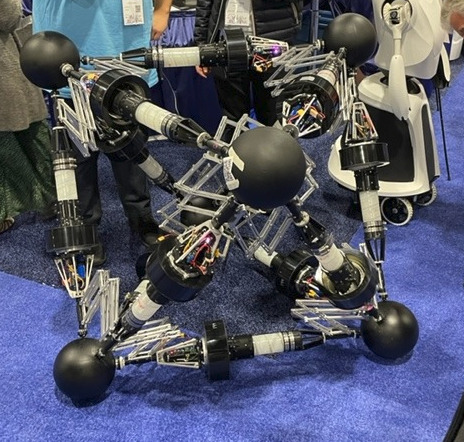
\includegraphics[width=.8\textwidth]{figures/truss.jpg}
			\end{tcolorbox}
		\end{column}	
	\end{columns}
	\centering \footnotesize{A multi-DOF Truss Robot. Courtesy of Penngineering (ICRA 2022, Philadelphia, PA).}
\end{frame}		
		
\begin{frame}
	\frametitle{Closed kinematic chains}
	\footnotesize{Connection degree $\ge 3$.}
	\newline
		\begin{columns}[b]
			\begin{column}{.74\columnwidth}			
				\begin{tcolorbox}[colframe=blue!80!green, coltitle=white!80,toggle enlargement=none]
					\centering 
					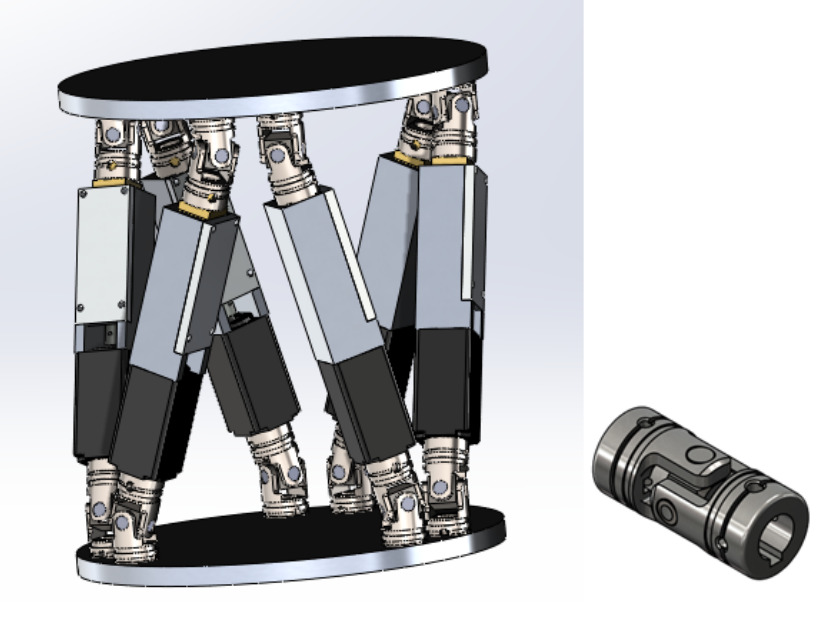
\includegraphics[width=\textwidth]{figures/stewart.jpg}
				\end{tcolorbox}
			\end{column}	
		\end{columns}
		\centering \footnotesize{A Stewart-Gough platform. SolidWorks Drawing Courtesy of Andrew Belcher. UChicago, 2018.}
\end{frame}

\begin{frame}
	\frametitle{A Soft Stewart Platform}
	\begin{columns}[b]
		\begin{column}{.8\columnwidth}		
			\begin{tcolorbox}[colframe=blue!80!green, coltitle=white!80,toggle enlargement=none]
				\centering 
				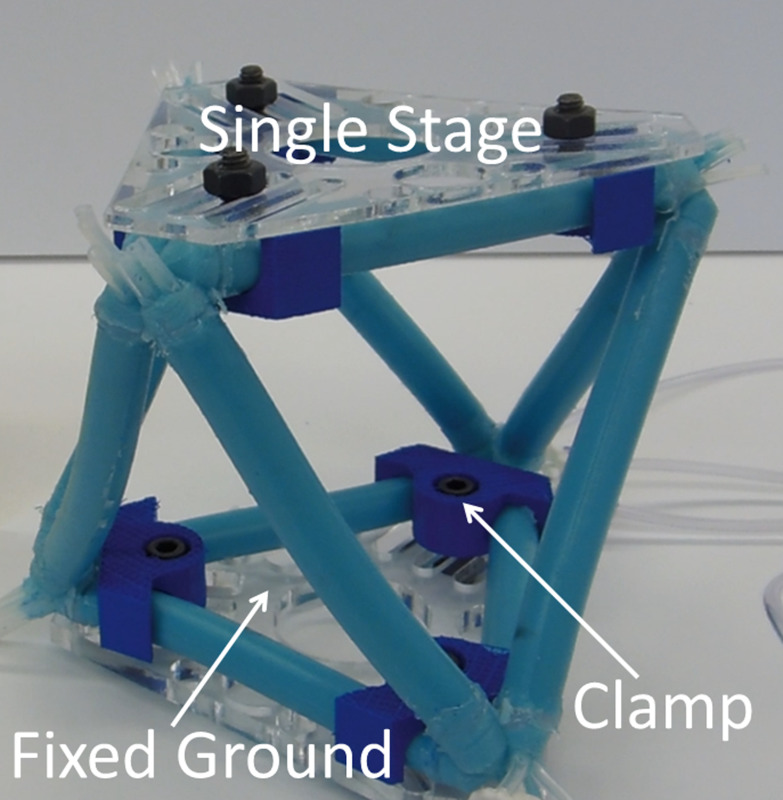
\includegraphics[width=.8\textwidth]{../Notes/figures/soft_parallel.jpg} 
			\end{tcolorbox} 
		\end{column}	
	\end{columns}
	\centering \footnotesize{A soft 6-6 Stewart manipulator. Jonathan Hopkins, 2015.}
\end{frame}



\lecture{Mobility and Freedoms}{Lecture II}
\section{Mobility}

\begin{frame}
	\frametitle{Outline}
	\begin{tcolorbox}[coltitle=yellow!50!black,colframe=magenta!25,split=.2,title=Freedom and Structure]
		Freedoms, Constraints, and Mobility.
		\tcblower
		Motion of linkages: Screws, and spatial motions.
		\vspace{.2cm}
		\newline
		Freedom and Mobility: Freedoms, unfreedoms, connectivity, mobility;
		\vspace{.2cm}
		\newline
		Gr{\"u}bler-Kutzbach's mobility criterion and examples.
	\end{tcolorbox}
\end{frame}
 


\begin{frame}
	\frametitle{Degrees of Freedom and Structure}
	%		
	\begin{definition}[Connection Degree]
		For any  \textcolor{blue}{manipulator joint}, we shall mean its \textcolor{red}{connection degree} to be the \textcolor{red}{number of links attached it}.
	\end{definition}
	%	
	\begin{block}{Quiz}
		What is the connection degree of the u-joints of a Stewart-Gough platform.
	\end{block}
\end{frame}

	\begin{frame}
	\frametitle{Members and Dual Graphs}			
	%
	\begin{tcolorbox}[colframe=blue!80!green, title=Dual graph of a Stewart platform, coltitle=white!80,toggle enlargement=none]
		\begin{columns}[b]
			\begin{column}{\linewidth}			
				\begin{figure}
					\centering 
					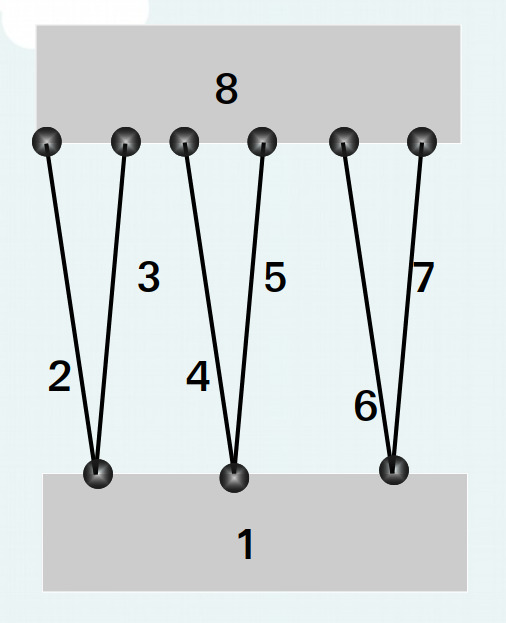
\includegraphics[width=.5\textwidth]{figures/dualgraph_stewart.jpg}
				\end{figure}
			\end{column}	
		\end{columns}
	\end{tcolorbox}
\label{fig:dualgraph}
\end{frame}

\begin{frame}
	\frametitle{Degrees of Freedom and Structure}
	%
	\begin{block}{Members and Freedoms}
		\textcolor{blue}{Degrees of freedoms (or freedoms)} concerns the \textcolor{red}{relative motion of members of a pair} that do not touch one another directly. 
	\end{block}
	%
	\begin{block}{Connectivity}
		By the dual graph of the Stewart platform as seen on Frame \autoref{fig:dualgraph}, the total number of freedoms that \textcolor{red}{connect the two members} (1 and 8) that do not connect to one another directly is \textcolor{blue}{six}. 
	\end{block}
\end{frame}


\begin{frame}
	\frametitle{Planar Linkages}	
	\begin{block}{Four Bar Linkages}
		\begin{columns}[b]
			\begin{column}{\linewidth}		
				\centering 
				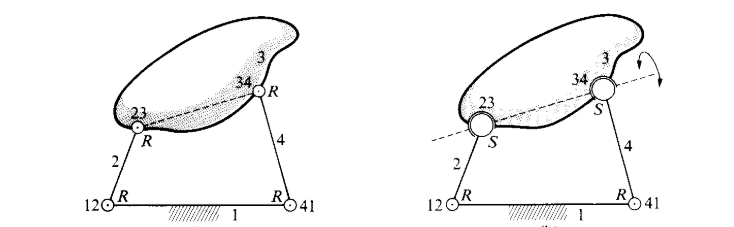
\includegraphics[width=\textwidth]{../Notes/figures/four-bar-linkage.png}
			\end{column}	
		\end{columns}
		\note{The planar $RRRR$ linkage, (\textit{left}) is modified in (\textit{right}) to an $RSSR$ linkage to allow spatial spin-movement of the coupler 3; the connectivity $\mathscr{C}_{13}=2$.}
		\footnotesize{Reprinted from Hunt, 1977: Kinematic Geometry of Mechanisms.}
	\end{block}
	\label{fig:4bar_hunt}
\end{frame}

\begin{frame}
	\frametitle{Freedom from Connectivity}			
	%
	\begin{tcolorbox}[colframe=blue!80!green, title=A (Hacked) Four-Bar Linkage, coltitle=white!80,toggle enlargement=none]
		\begin{columns}[b]
			\begin{column}{.45\linewidth}			
				\begin{figure}
					\centering 
					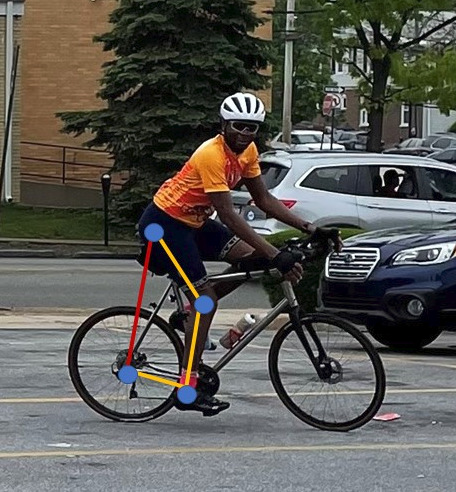
\includegraphics[width=\textwidth]{figures/4bar_me.jpg}
				\end{figure}
			\end{column}
		\begin{column}{.45\linewidth}			
			\begin{figure}
			\centering 
			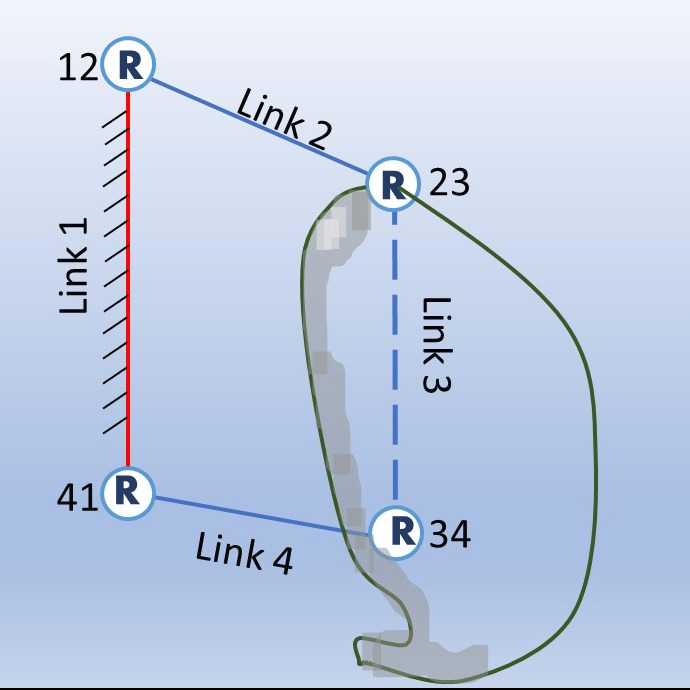
\includegraphics[width=\textwidth]{figures/4bardual.jpg}
			\end{figure}
		\end{column}	
		\end{columns}
	\end{tcolorbox}
	\label{fig:4bar}
\end{frame}


\begin{frame}
	\frametitle{The Four Bar Linkage}
	%
	\begin{block}{Couplings and Freedom}
		
		Links $2 \& 4$ complete a \textcolor{cyan}{coupling or connection} between links $1 \& 3$. 
	\end{block}
	%
	\begin{block}{Connectivity}
		The $R$-pairs are said to have a \textcolor{magenta}{connectivity} of  $\mathscr{C}_{ij}=1$ for all $i,j=1,2,3,4$. Thus, total degree of freedom is $1$.
	\end{block}
\end{frame}

\begin{frame}
	\frametitle{Mobility of Mechanisms}
	%
	\begin{block}{The Mobility and Relative Mobility, $\mathfrak{M}$}
		Simply put, the number of a mechanism's freedoms is its \textcolor{cyan}{mobility}, or \textcolor{cyan}{relative mobility},  $\mathfrak{M}$.  
	\end{block}
	%
	\begin{block}{The Mobility, $\mathfrak{M}$}
		It specifies the \textcolor{green}{independent variables} needed to \textcolor{pink}{determine every relative location} of a \textcolor{red}{mechanism's members}  with respect to one another.
	\end{block}
	%
	\begin{block}{A Note on Serial and Parallel Mobility}
		A little tricky to determine for parallel mechanisms but straightforward for serial mechanisms.
	\end{block}
\end{frame}

\begin{frame}
	\frametitle{Mobility of Mechanisms}
	%
	\begin{block}{Quiz}
		What is the mobility $\mathfrak{M}$ of the $RSSR$ four bar linkage of Frame \ref{fig:4bar_hunt}? Why?
	\end{block}
	%
	\begin{block}{Quiz}
		What is the mobility $\mathfrak{M}$ of the $RRRR$ four bar linkage of Frame \ref{fig:4bar}? Why?
	\end{block}
	%
	\begin{definition}[The mobility criterion (well, not yet)]
		Let's not get ahead of ourselves. A little introduction to screws are in order for us to grasp the \textcolor{red}{Gr{\"u}bler-Kutzbach} mobility criterion.
	\end{definition}
\end{frame}


\subsection{Screws}
\begin{frame}
	\frametitle{Unique Location of a Rigid Body in 3D Space}
	%
	\begin{tcolorbox}[top=0mm, title=Inhomogeneity of Displacements and Angles]
		Quiz: Three translations and three rotations are ill-posed for uniquely determining the freedoms of a body. Why?
		\tcblower
		They are \textcolor{green}{not homogeneous}. 
		\begin{description}
			\item For true \textcolor{blue}{kinematic wholeness and generality}, displacement that is \textcolor{red}{purely translatory} and \textcolor{red}{purely rotary} is needed.
		\end{description}
	\end{tcolorbox}
\end{frame}

\begin{frame}
	\frametitle{Screws for Kinematic Generality}
	%
	\begin{block}{Need for Screws}
		From a kinematic standpoint, \textcolor{red}{six homogeneous screw coordinates} -- each having an \textcolor{cyan}{independent screw freedom} -- are needed to \textcolor{red}{uniquely determine a rigid body's location}.
	\end{block}
	%
	\begin{columns}[b]
		\begin{column}{.7\columnwidth}
			\begin{definition}[What is a screw anyway?]
				A \textcolor{blue}{screw} is a \textcolor{red}{straight line} in space, called \textcolor{blue}{the axis}, with an associated direction, called \textcolor{blue}{pitch}, $p$.
			\end{definition}
		\end{column}
		\begin{column}{.25\columnwidth}
			\centering
			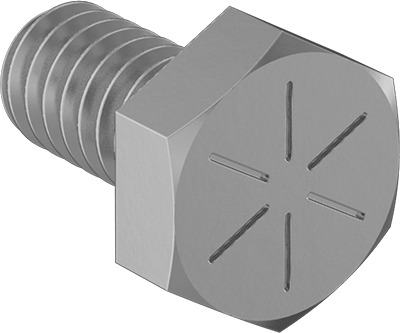
\includegraphics[width=\textwidth]{figures/screw.jpg}
		\end{column}
	\end{columns}
\end{frame}

\begin{frame}
	\frametitle{Unique Location of a Rigid Body in 3D Space}
	%
	\begin{columns}[b]
		\begin{column}{.65\columnwidth}
			\begin{definition}[Screw Coordinates]
				Six-vector, $\bm{s}$, related to the Pl{\"u}cker coordinates (see right inset) parameterize a screw i.e. $\bm{s}=\left(s_1, s_2, s_3, s_4, s_5, s_6\right)$.
			\end{definition}
		\end{column}
		\begin{column}{.3\columnwidth}
			\centering
			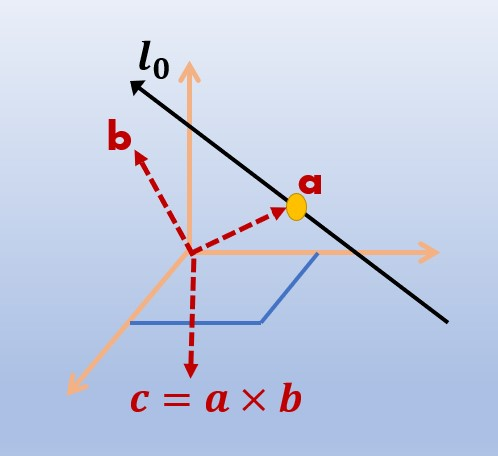
\includegraphics[width=\textwidth]{figures/plucker_coords.jpg}
		\end{column}
		\label{fig:plucker}
	\end{columns}
	%
	\begin{block}{Pl{\"u}cker Coordinates}
		Let \textcolor{red}{$\bm{a}$} be a point on line $\bm{\ell}_0$. Let \textcolor{red}{$\bm{a}$}'s direction cosine vector (to be introduced shortly) be \textcolor{red}{$\bm{b}$}. Then, its binormal (moment) vector is \textcolor{red}{$\bm{c=a\times b}$}. We say the pair \textcolor{red}{$(\bm{b},\bm{c})$} is the \textcolor{blue}{Pl{\"u}cker Coordinates} of the point  \textcolor{red}{$\bm{a}$ on axis $\bm{\ell}_0$}.
	\end{block}
\end{frame}


\subsection{Pl{\"u}cker coordinates}
\begin{frame}
	\frametitle{Screws and Pl{\"u}cker Coordinates Relationship}
	%
	\begin{block}{Screw axis and Pl{\"u}cker Coordinates Relationship}
		\begin{align}
			b_1 &= s_1, \quad b_2 = s_2, \quad b_3 = s_3 \\
			c_1 &= s_4 - ps_1, \quad c_2 = s_5-ps_2, \quad c_3 = s_6 - ps_3.
		\end{align}
	$p$: pitch! How to find it?
	\end{block}
	%
	\begin{block}{Screw and Pl{\"u}cker Coordinates Relationship}
		Suppose that 
		\begin{align}
			h &= \sqrt{b_1^2+b_2^2+b_3^2}.
		\end{align}
		Then $(\bm{b}/h, \bm{c}/h)$ are respectively the direction cosines of the line, $l_0$ and its moment.
	\end{block}
\end{frame}

\begin{frame}
	\frametitle{Pitch and Magnitude of the screw}	
	\begin{block}{Pitch of a screw}
		\begin{align}
			p &= \dfrac{s_1 \, s_4 + s_2 \, s_5 + s_3 \, s_6}{\sqrt{s_1^2 + s_2^2 + s_3^2}}, \\
			\mid s \mid &= \sqrt{s_1^2 + s_2^2 + s_3^2} \quad \text{if } p \neq \infty \\
			\mid s \mid &= \sqrt{s_4^2 + s_5^2 + s_6^2} \quad \text{if } p = \infty
		\end{align}
	\end{block}
\end{frame}
%
\begin{frame}
	\frametitle{Pl{\"u}cker Coordinates Example}
	\begin{block}{Chasles' Theorem Applied to The Serret-Frenet Frame}
		Consider a spatial curve $\bm{C}$ on the elephant continuum trunk shown earlier. Suppose $\bm{C}$ is parameterized by its arc length $\bm{s} \in [0, 1]$. For a point $\bm{x}=\left[x, y, z\right]^T$ on $\bm{C}$, the unit tangent vector to $\bm{C}$ is $\bm{t}=\bm{dx}/\bm{ds}$. Denote by $\bm{n}$ the principal normal to $\bm{C}$ at $\bm{n}$; then we must have $\bm{b}=\bm{t}\times \bm{n}$ as the binormal. We say $(\bm{b},\bm{n})$ together form the Pl{\"u}cker coordinates of the tangent $\bm{t}$.
	\end{block}
	%
	%
	\begin{columns}[]
		\begin{column}{.5\columnwidth}
			\centering
			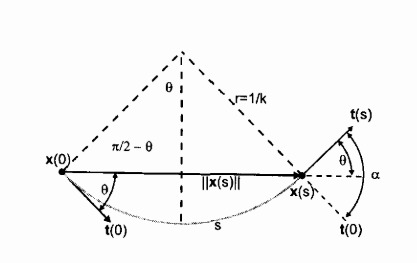
\includegraphics[width=\textwidth]{figures/serret.jpg}
		\end{column}
	\end{columns}
\end{frame}

\begin{frame}
	\frametitle{Pl{\"u}cker Coordinates Example}
	%
	\begin{block}{Poinsot's Theorem Quiz on a  Force and its Moment}
		Suppose that a force $\bm{F}$  acts at the point $\bm{a}$ in the image of Frame \ref{fig:plucker}. What are the Pl{\"u}cker coordinates of the \textcolor{red}{line of force}?
	\end{block}
	%
	\begin{block}{ Homogeneous Coordinates!}
		\textcolor{blue}{Pl{\"u}cker Coordinates} give six unit parameters of a point on a line. Pl{\"u}cker Coordinates are in \textcolor{red}{homogeneous coordinates}!
	\end{block}
\end{frame}

\note{
\begin{frame}
	%
	\begin{block}{Poinsot's Theorem Quiz on a  Force and its Moment}
		Imagine that a force $\bm{F}$ is acting at the point $\bm{a}$ in the image of Frame \ref{fig:plucker}. Suppose that $\bm{\tau}$ is torque acting along the normal to point $\bm{a}$.  Then $(\bm{f,\tau})$ are the Pl{\"u}cker  coordinates of the \textcolor{red}{line of force}.
	\end{block}
	%
	\begin{block}{Arithmetics on Screws}
		Scalar and vector arithmetic operations are valid on infinitesimal  screws e.g.
		\begin{align}
			c_1 \bm{s}_1 + c_2 \bm{s}_2 = 0 \text{ for } c_1, \, c_2 \neq 0 \text{ on screws } \bm{s}_1, \bm{s}_2.
		\end{align}
	\end{block}
\end{frame}
}

\subsection{Freedoms and Constraints}
\begin{frame}
	\frametitle{Freedoms, Unfreedoms, and Mobility}
	%
	\begin{block}{Freedom and Constraints}
		Suppose a screw $\bm{f}=(f_1,\cdots, f_6)$ ``fixes" a body in 3D space. 
		\begin{description}
			\item Each \textcolor{red}{constraint} $u_i \neq f_j$ for $(i,j)\in \{1,\cdots,6\}$.
			%
			\item Rather each \textcolor{red}{$u_i$} has influence on every $\{f_i\}_{i=1}^{6}$.
			%
			\item Each $u_i$ from the six independent equations, $g(s_1, s_2, s_3, s_4, s_5, s_6)=0$, suppresses a \textcolor{cyan}{freedom}, $f_i$.
			%
			\item Progressively relaxing each \textcolor{red}{$u_i$}, \textcolor{red}{or unfreedom}, adds an extra body $f_i$.
		\end{description}
	\end{block}
	%
\end{frame}


\begin{frame}
	\frametitle{Freedoms, Unfreedoms, and Mobility}
	%
	\begin{block}{Freedom and Unfreedoms}
		Suppose the total \textcolor{blue}{freedoms} is $\bm{f}$ and the total \textcolor{red}{unfreedoms} is $\bm{u}$, then
		\begin{description}
			\item $\bm{u}+\bm{f}=6.$
			\label{eq:freedomunfreedom}
		\end{description}
	Note: A rigid body's freedoms is also referred to the dimension of  its \textcolor{blue}{configuration space}.
	\end{block}
	%
	\begin{block}{Relative Freedoms}
		Suppose there are a total of $n$ \textcolor{red}{unconstrained} bodies. Suppose further that we choose one out of the bodies as a reference body. Then the total number of \textcolor{green}{relative freedoms} is $6(n-1)$.
	\end{block}
\end{frame}

\begin{frame}
	\frametitle{Freedoms, Unfreedoms, and Mobility}
	\begin{block}{Constraints and Joints}
		Now, consider $k$ \textcolor{red}{independent constraints}\footnote{NB: The total \textit{allowable} constraints is 5 for a body in relative motion. It is 6 for a fully rigid body.} such as \textcolor{blue}{joints} \textcolor{green}{along points, lines, curves or surfaces}.
	\end{block}
	
	\begin{block}{The Mobility Criterion}
		Let the \textcolor{red}{constraint} of joint, $i$ (e.g. a joint along points, lines, curves or surfaces) be $u_i$. Then the mobility criterion $\mathfrak{M}$ is
		\begin{align}
			\mathfrak{M}=6(n-1) - \sum_{i=1}^{k}u_i.
		\end{align}
	\end{block}
\end{frame}

\subsection{Mobility Criterion}

\subsection{Mobility Criterion}
\begin{frame}
	\frametitle{ General Gr{\"u}bler-Kutzbach Mobility Criterion}	
	\begin{block}{ General Gr{\"u}bler-Kutzbach Mobility Criterion}
		Recall that $\sum_i u_i + f_i = 6$ from Frame \eqref{eq:freedomunfreedom} so that 
		\begin{align}
			\mathfrak{M}=6(n-k-1) - \sum_{i=1}^{f}f_i.
			\label{grubler}
		\end{align}
	\end{block}
	
	\begin{block}{Exceptions: Relative Planar and Spherical Motions}
		For bodies restricted to relative planar or spherical  motions, the total freedoms + constraints is 3 (not 6)! %Therefore, 
		\begin{align}
			\mathfrak{M}=3(n-k-1) - \sum_{i=1}^{f}f_i.
			\label{grubler}
		\end{align}
	\end{block}
\end{frame}

\begin{frame}
	\frametitle{ General Gr{\"u}bler-Kutzbach Criterion References}
		
	\begin{block}{The Gr{\"u}bler-Kutzbach Mobility Criterion References}
		Attributed to Gr{\"u}bler: 
		\begin{description}
			\item \footnotesize{Schoenflies, Arthur, and M. Grübler. ``Kinematik." In Encyklopädie der Mathematischen Wissenschaften mit Einschluss ihrer Anwendungen, pp. 190-278. Vieweg+Teubner Verlag, Wiesbaden, 1908};
			\item \footnotesize{Grübler, Martin Fürchtegott. Getriebelehre: eine Theorie des Zwanglaufes und der ebenen Mechanismen. Springer, 1917}.
		\end{description}
	and Kutzbach:
		\begin{description}
			\item \footnotesize{Kutzbach, Karl. "Mechanische leitungsverzweigung, ihre gesetze und anwendungen." Maschinenbau 8, no. 21 (1929): 710-716.}
		\end{description}
	\end{block}
\end{frame}

\begin{frame}
	\frametitle{Loops}	
	\begin{block}{Loops}
		A \textcolor{blue}{kinematic chain} often comprises \textcolor{blue}{members} called \textcolor{green}{loops}. 
	\end{block}
	
	\begin{block}{Binary Link}
		Members in a \textcolor{blue}{binary link} constitute a \textcolor{green}{single loop}. Example: The four-bar linkage. 
	\end{block}	
	
	\begin{block}{Single loops}
		For \textcolor{blue}{single loops}, $k=n$ so that $\mathfrak{M}=\sum_{i=1}^{f} f_i - 6$. 
	\end{block}
	
	\begin{block}{Mobility of Mechanisms}
		$\mathfrak{M}\le 1$ for at least one actuator-pair to produce mobility at a successor joint which depends on that actuator-pair's input. 
	\end{block}
\end{frame}


%
\begin{frame}
	\frametitle{Mobility of Common Robot Configurations}
	%
	\begin{columns}[]
		%
		\begin{column}{.5\linewidth}
			\centering
			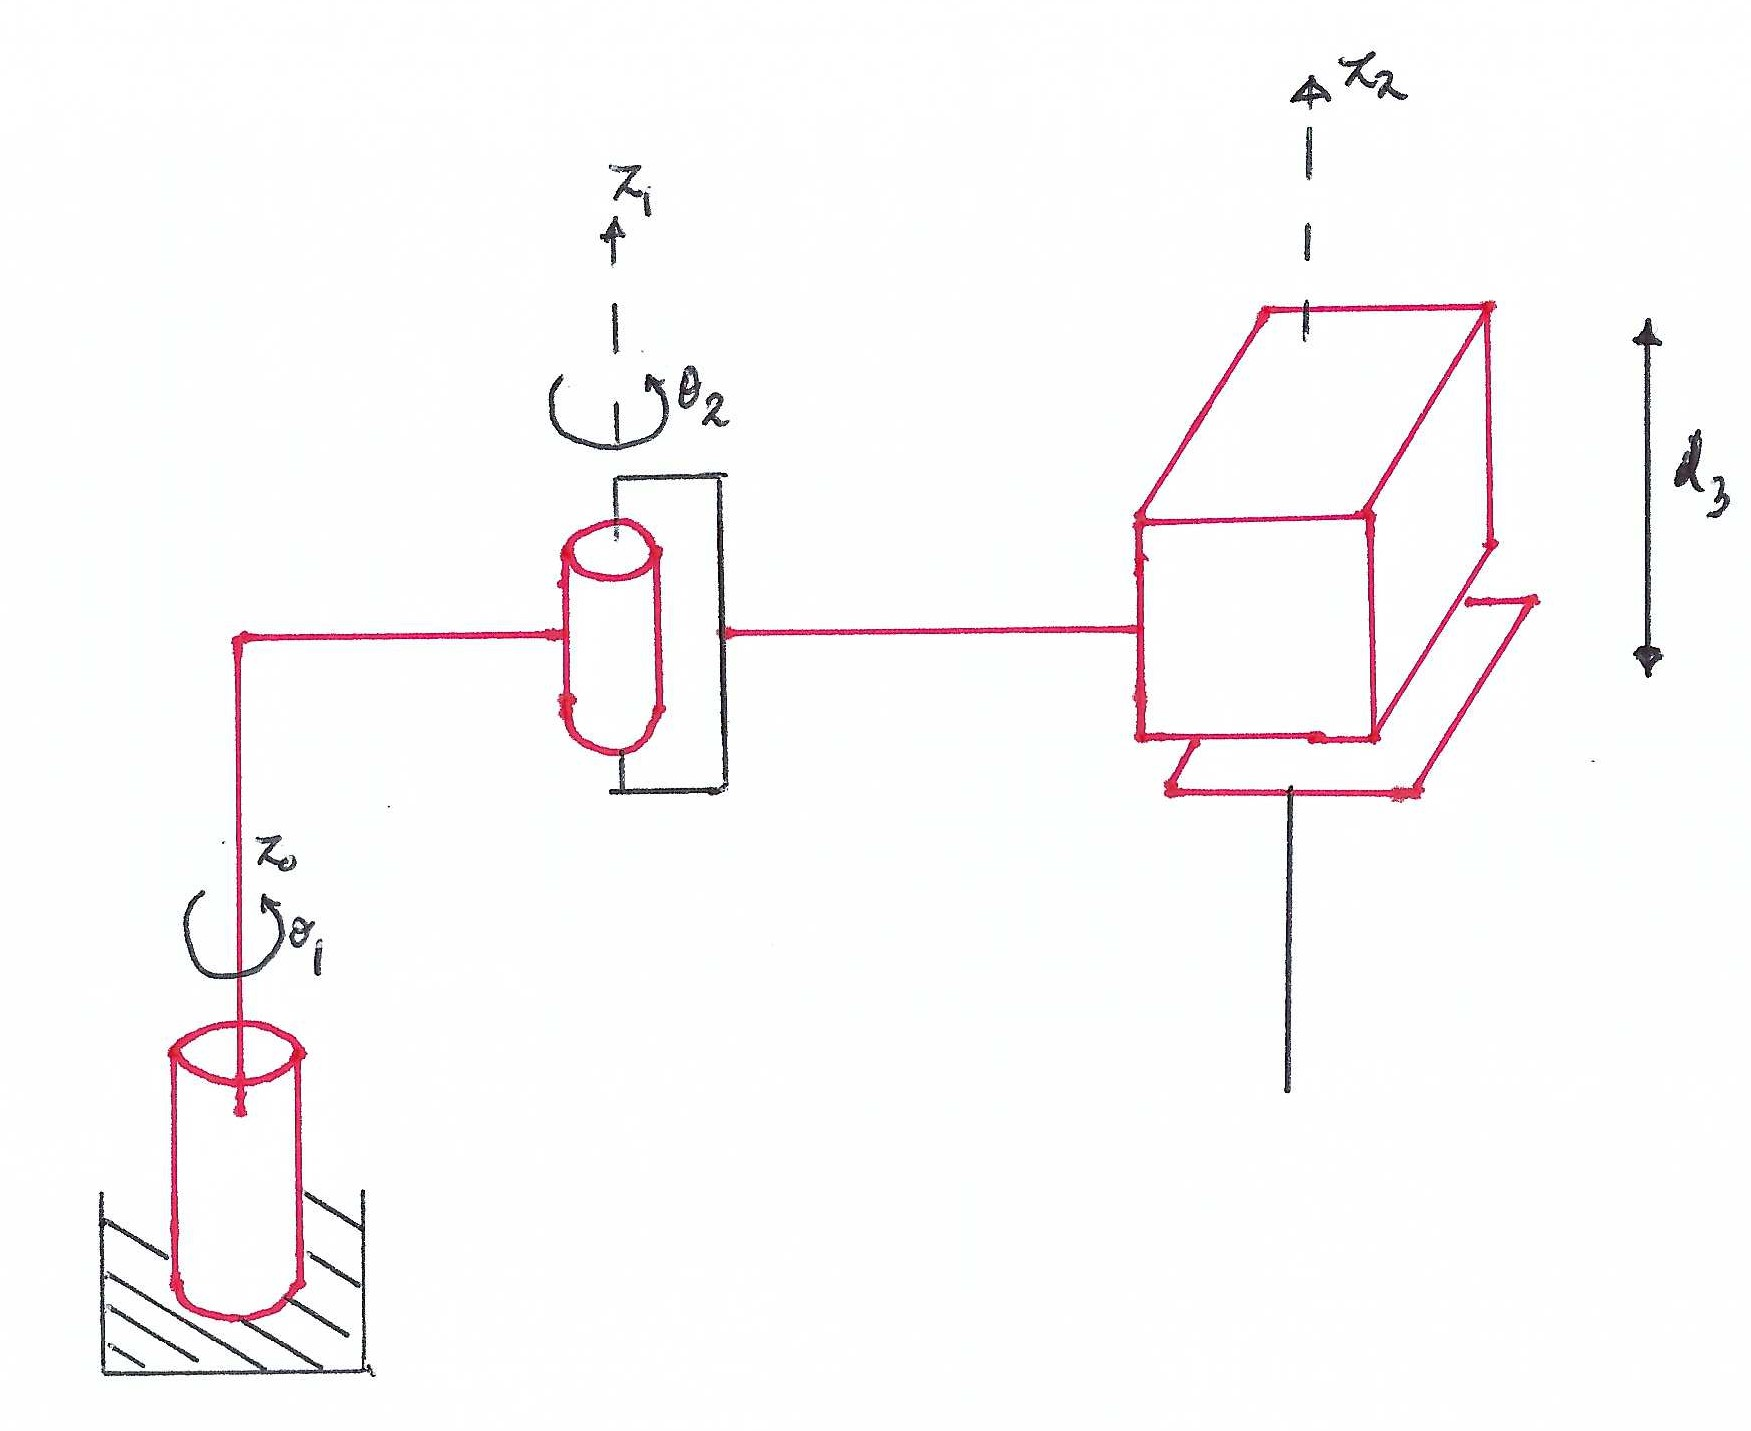
\includegraphics[width=\textwidth]{figures/scara_schematic.jpg}
			\footnotesize{Configuration of the SCARA Arm.}
		\end{column}
		%
		\begin{column}{.5\linewidth}
			\centering
			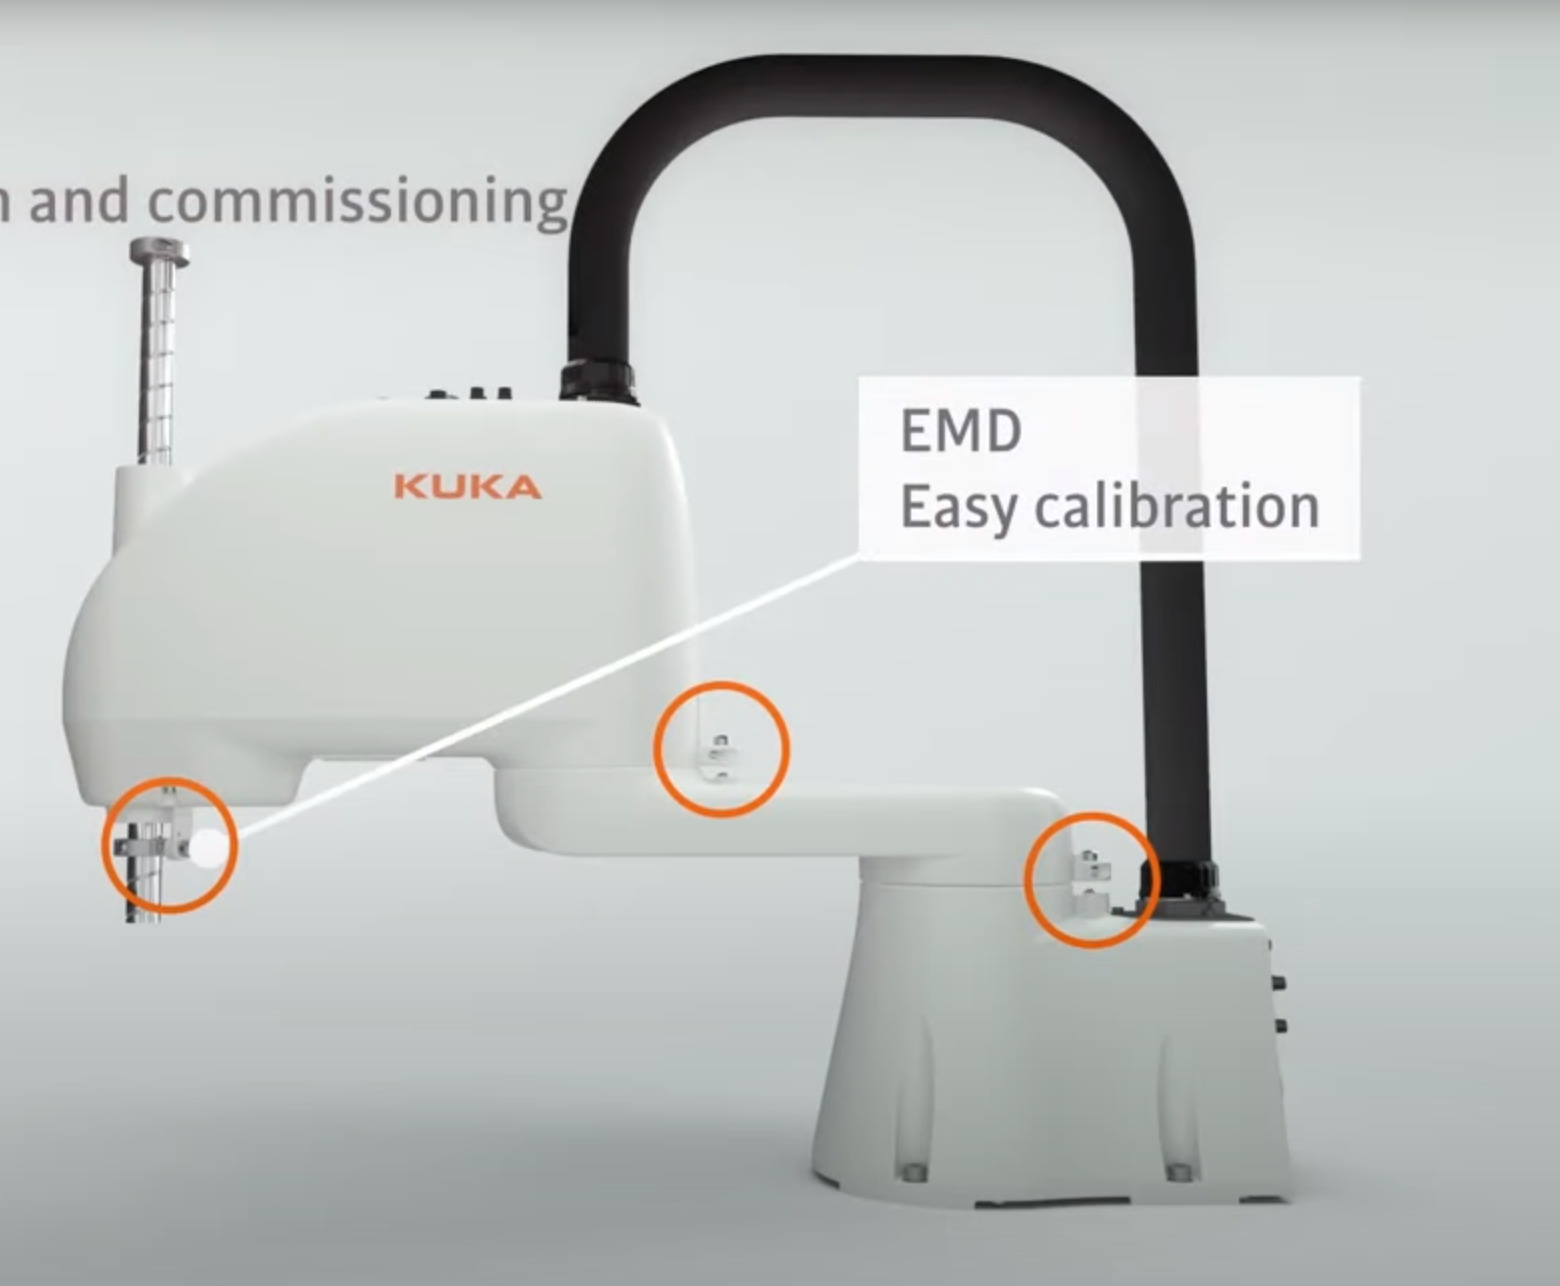
\includegraphics[width=\textwidth, rotate=360]{figures/Scara.jpg}
			\footnotesize{Courtesy of Fanuc America Inc.}
		\end{column}
	\end{columns}
\end{frame}
%
\begin{frame}
	\frametitle{Mobility of The SCARA Robot}
	%
	\begin{columns}[]
		%
		\begin{column}{.5\linewidth}
			\begin{block}{Mobility Analysis}
				Two rotary joints. One prismatic joint acting along the $z$ axis, and constrained along the $xy$ plane. 
			\end{block}
		\end{column}
	%
		\begin{column}{.5\linewidth}
			\begin{block}{Mobility Parameters}			
			Four rigid bodies (links). Three constraints.  Four freedoms. Therefore, $\mathfrak{M}=6(4-3-1)+4=4$
			\end{block}
		\end{column}
	\end{columns}
\end{frame}

\begin{frame}
	\frametitle{Mobility Analysis of The Universal Robot}
	%
	\begin{columns}[]
		%
		\begin{column}{.5\linewidth}
			\centering
			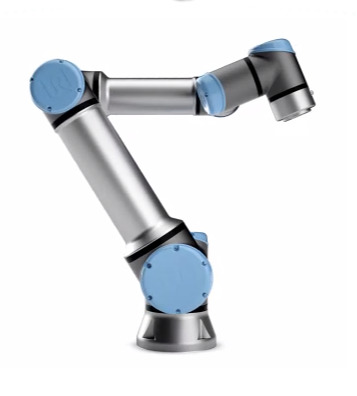
\includegraphics[width=\textwidth]{figures/ur16.jpg}
			\footnotesize{\copyright Universal Robots A/S, DK.}
		\end{column}
		%
		\begin{column}{.5\linewidth}
			\centering
			\begin{block}{The Revolute Arm}
				\footnotesize{Falls under so-called $RRR$ kinematic arrangements. Also called a \textcolor{blue}{revolute}, \textcolor{blue}{elbow}, or \textcolor{blue}{anthorpomorphic manipulator}.}
			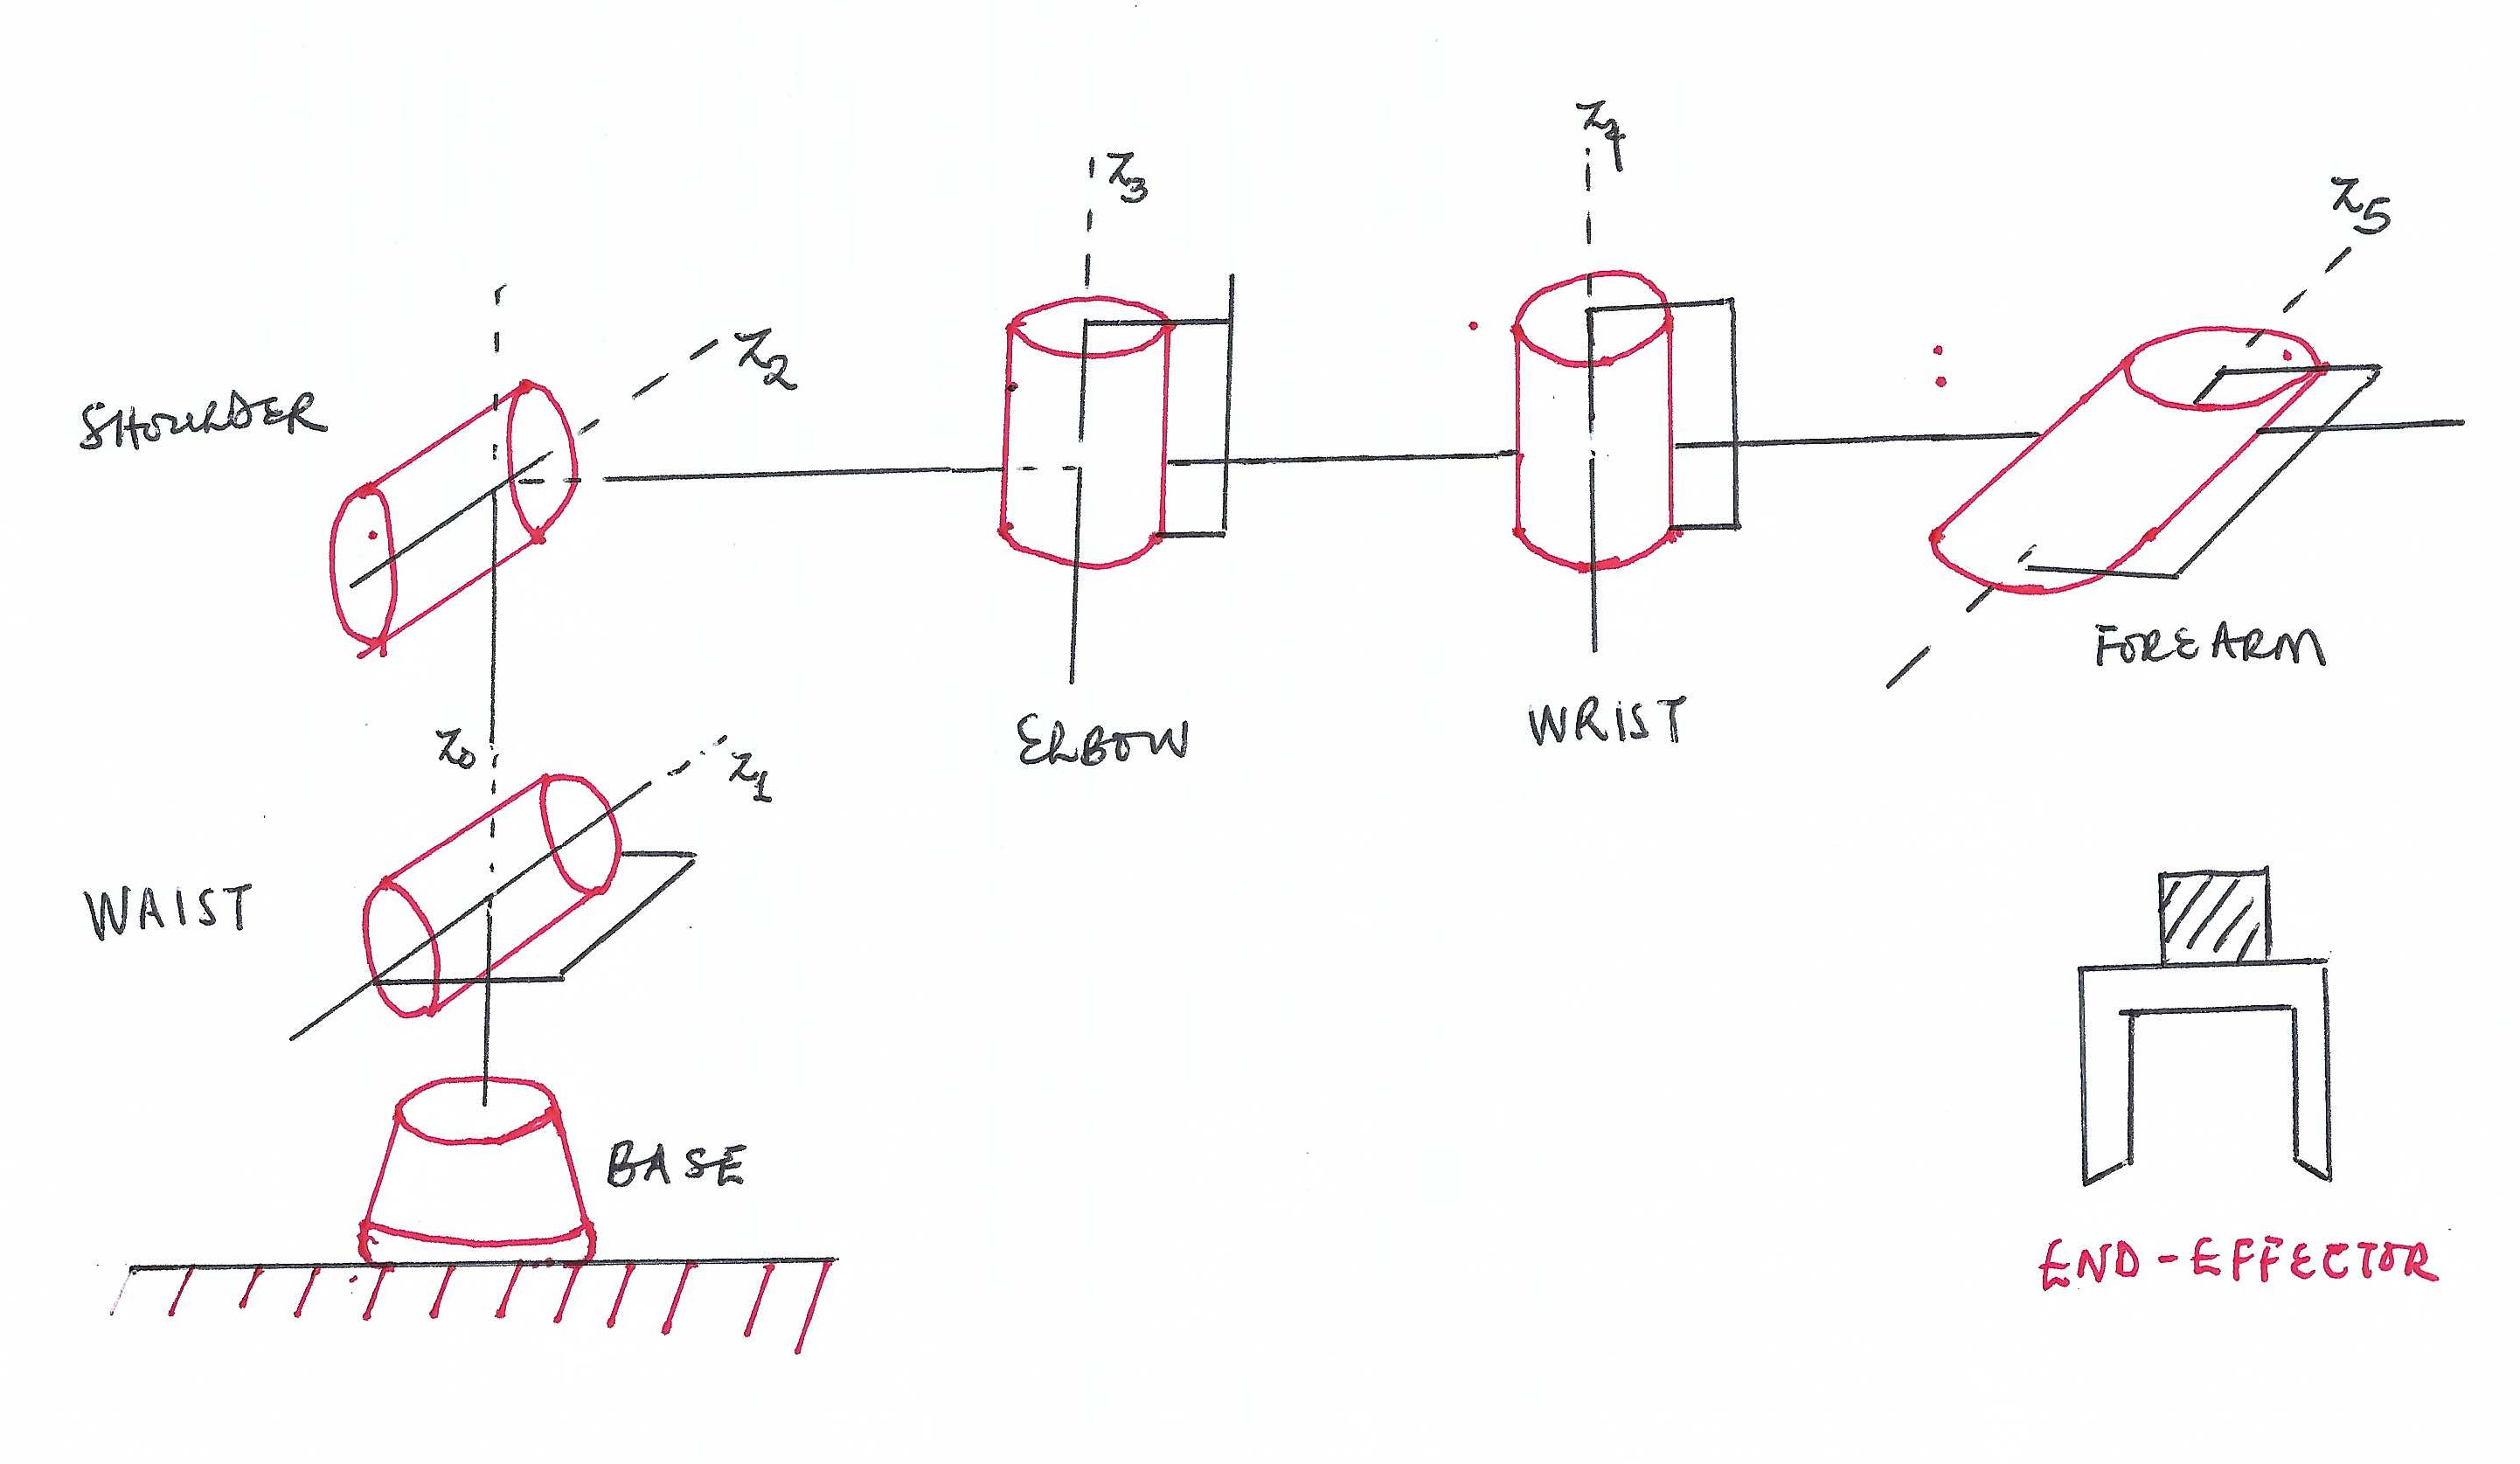
\includegraphics[width=\textwidth]{figures/ur_scheme.jpg}
			$n=6; \, k=6; \, f=5\times3:=18$ $\therefore \mathfrak{M}=6(n-k-1)+\sum f_i $ $\implies 6(6-1-5) + 18$ or $\mathfrak{M}=6$.
			\end{block}
		\end{column}
	\end{columns}
\end{frame}

\begin{frame}
	\frametitle{Mobility of The Stewart-Gough Platform}
	%	
	\centering 
	\begin{columns}
		\begin{column}{.4\linewidth}
			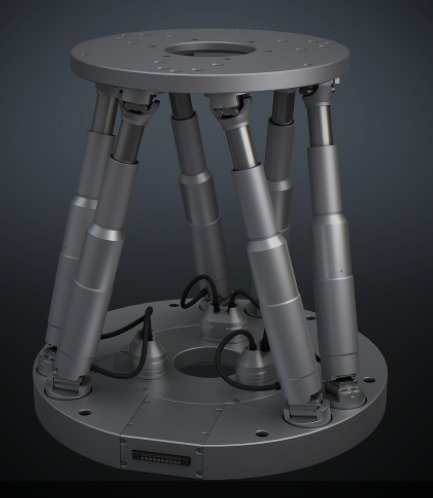
\includegraphics[width=\textwidth]{figures/stewart_spherical.jpg}
		\end{column}
		%\begin{columns}
		\begin{column}{.25\linewidth}
			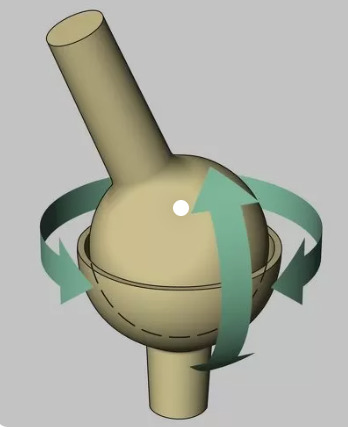
\includegraphics[width=\textwidth]{figures/spherical.jpg}
			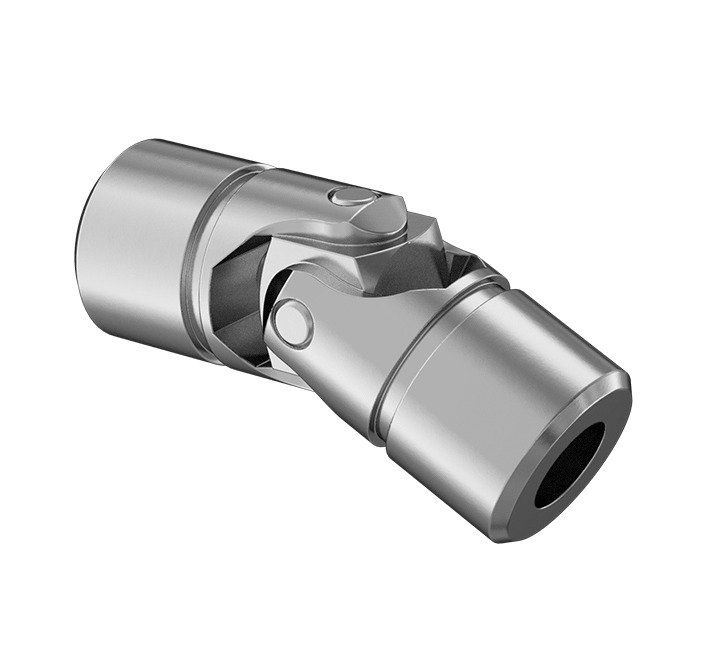
\includegraphics[width=\textwidth]{figures/ujoint.jpg}	
		\end{column}
		%\end{columns}
	\end{columns}	
\end{frame}

\begin{frame}
	\frametitle{Mobility of The Stewart-Gough Platform}
	%
	\begin{columns}[]
		%
		\begin{column}{.45\linewidth}
			\begin{block}{Unconstrained bodies, $n$}
				There are \textcolor{blue}{six universal joints} that connect \textcolor{blue}{the base platform} to the prismatic linear actuators. There are \textcolor{blue}{six spherical joints} that connect \textcolor{blue}{the top platform} to the top of the prismatic actuators. Altogether, there are $n=6+6+2$ or $14$ unconstrained \textcolor{red}{rigid links}.
			\end{block}
		\end{column}
		%
		\begin{column}{.55\linewidth}
			\begin{block}{Constraints, $k$}			
				Six \textcolor{blue}{u-joints}. Six \textcolor{blue}{spherical joints}.  Six \textcolor{blue}{prismatic joints}. Altogether, there are $f=6+6+6:=18$ \textcolor{blue}{constraints}.
			\end{block}
			\begin{block}{Freedoms, $f$}			
				Each \textcolor{blue}{u-joints has two freedoms}. Each \textcolor{blue}{spherical joint has three (rotary) freedoms}.  Each \textcolor{blue}{prismatic joint has one freedom}. Altogether, there are $f=6\times2+6\times3+6\times1:=36$ \textcolor{blue}{freedoms}.
			\end{block}
		
		\end{column}
	\end{columns}
\end{frame}

\lecture{Rigid Body Motions}{Lecture III}
\begin{frame}
	\frametitle{Lecture III Outline}
	\begin{tcolorbox}[coltitle=yellow!50!black,colframe=magenta!25,split=.2,title=Rigid Body Motions]
		Screws and Rigid Body Transformations.
		\tcblower
		Rigid body motions:Properties; Direction cosines; Rotation compositions.
		\vspace{.2cm}
		\newline
		Screws (properly revisited): Chasles' and Poinsot's theorem.
		\vspace{.2cm}
		\newline
		Displacement and Force screws; Pl{\"u}cker coordinates; Homogeneous coordinates;
		\vspace{.2cm}
		\newline
		Rodrigues' formula; the matrix exponential.
	\end{tcolorbox}
\end{frame}

\begin{frame}
	\frametitle{Lecture III Outline}
	\begin{tcolorbox}[coltitle=yellow!50!black,colframe=magenta!25,split=.2,title=Rigid Body Motions]
		Screws and Rigid Body Transformations.
		\tcblower
		Group theory: The Lie algebra, motions in $\mathfrak{se}(3)$;, and the Lie Group.
		\vspace{.2cm}
		\newline
		Transformations: Translations and rotations in $\mathbb{R}^3$, planar rotations, $SO(3), SE(3)$ motions;  homogeneous transformations; Euler and Fick angles; Brockett's exponential map formula. Paden-Kahan subproblems.
	\end{tcolorbox}
\end{frame}

\begin{frame}
	\frametitle{Rigid Body Motions}
	%
	\begin{block}{Rigid Body Motion -- Intro}
		A mapping $g:  \mathbb{R}^3  \rightarrow \mathbb{R}^3$ is a \textcolor{red}{rigid body motion} if 
		\begin{align}
			\|g({x}) - g({y})\| &= \|{x} - {y}\| \text{ for all }  {x}, {y} \in \mathbb{R}^3;  \\
			g({x} \times {y}) &= g(x) \times g({y})\text{ for all }  {x}, {y} \in \mathbb{R}^3; 
		\end{align}
	\end{block}	
	%
	\begin{block}{Rigid Body Motion Preserves Inner Products}
		For two vectors $\bm{a}$ and $\bm{b}$,  $\langle \bm{a},  \bm{b}\rangle =  g(\bm{a}) \times  g(\bm{b})$.
	\end{block}
\end{frame}

\begin{frame}
	\frametitle{Rigid Body Motions as Screws}
	%
	\begin{block}{Rigid Body Motion as a Screw Motion}
		The motion of a \textcolor{red}{rigid body} is precisely the same as if it were attached to  the \textcolor{red}{nut of a literal mechanical screw}. Associated with the screw is its pitch.
	\end{block}	
	%
	\begin{definition}[Screw]
		That straight line with which a \textcolor{red}{definite linear magnitude} termed the pitch is associated is called the \textcolor{red}{screw}.
	\end{definition}
\end{frame}


\begin{frame}
	\frametitle{Screw as a Geometric Quantity}	
	%	
	\begin{block}{Pitch of a Screw}
		\textcolor{brown}{The rectilinear distance}  through which (a literal nut)  \textcolor{red}{nut is translated parallel to the axis of a screw}, while the nut is rotated through the \textcolor{cyan}{angular unit of circular measure} is termed the \textcolor{light-blue}{pitch}.
	\end{block}
	%
	\begin{block}{Pl{\"u}cker Coordinates}
		Let \textcolor{red}{$\bm{a}$} be a point on line $\bm{\ell}_0$. Let \textcolor{red}{$\bm{a}$}'s direction cosine vector (to be introduced shortly) be \textcolor{red}{$\bm{b}$}. Then, its binormal (moment) vector is \textcolor{red}{$\bm{c=a\times b}$}. We say the pair \textcolor{red}{$(\bm{b},\bm{c})$} is the \textcolor{blue}{Pl{\"u}cker Coordinates} of point  \textcolor{red}{$\bm{a}$ on axis} $\bm{\ell}_0$.
	\end{block}	
\end{frame}

\begin{frame}
	\frametitle{Screw in Pl{\"u}cker Coordinates}
	%
	\begin{columns}[b]
		\begin{column}{.67\columnwidth}
			\centering
			\begin{definition}[Screw Coordinates]
				Six-vector, $\bm{s}$, related to the Pl{\"u}cker coordinates, parameterize a screw i.e. $\bm{s}=\left(s_1, s_2, s_3, s_4, s_5, s_6\right)$.
			\end{definition}
		\end{column}
		
		\begin{column}{.3\columnwidth}
			\centering
			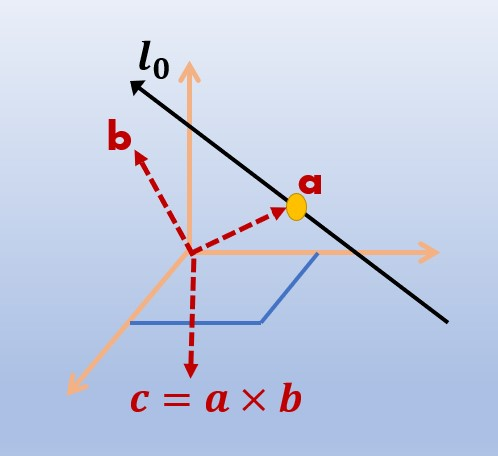
\includegraphics[width=\textwidth]{figures/plucker_coords.jpg}
		\end{column}
		\label{fig:plucker}
	\end{columns}
\end{frame}


\subsection{Displacement \& Twist}
\begin{frame}
	\frametitle{Screws and Pl{\"u}cker Coordinates}
	%
	\begin{block}{Screw axis and Pl{\"u}cker Coordinates}
		\begin{align}
			b_1 &= s_1, \quad b_2 = s_2, \quad b_3 = s_3; \\
			c_1 &= s_4 - p \cdot s_1, \quad c_2 = s_5-p\cdot s_2, \quad c_3 = s_6 - p\cdot s_3.
		\end{align}
	\end{block}
	%
	\begin{block}{Pitch in Pl{\"u}cker Coordinates}
		\begin{align}
			p &= \dfrac{s_1 \, s_4 + s_2 \, s_5 + s_3 \, s_6}{{s_1^2 + s_2^2 + s_3^2}}, \\
			\mid s \mid &= \sqrt{s_1^2 + s_2^2 + s_3^2} \quad \text{if } p \neq \infty, \\
			\mid s \mid &= \sqrt{s_4^2 + s_5^2 + s_6^2} \quad \text{if } p = \infty
		\end{align}
	\end{block}
\end{frame}


\begin{frame}
	\frametitle{Pitch and Magnitude of the screw}	
	\begin{block}{Pl{\"u}cker Coordinates' Direction Cosines}
		Suppose that 
		%\begin{align}
		$h = \sqrt{b_1^2+b_2^2+b_3^2}$.
		%\end{align}
		Then $(\bm{b}/h, \bm{c}/h)$ are respectively the direction cosines of the line, $l_0$ and its moment.
	\end{block}
	%
	\begin{block}{ Homogeneous Coordinates!}
		\textcolor{blue}{Pl{\"u}cker Coordinates} give six unit parameters of a point on a line. Pl{\"u}cker Coordinates are in \textcolor{red}{homogeneous coordinates}!
	\end{block}
\end{frame}

\begin{frame}
	\frametitle{Twist About a Screw (Axis)}
		%
		\begin{block}{Twist}
			A body's \textcolor{purple}{twist} about 
			s \textcolor{magenta}{screw} is a \textcolor{red}{uniform (infinitesimal) rotation} about the screw \textcolor{blue}{followed by a uniform (infinitesimal) translation} about an \textcolor{cyan}{axis parallel to the screw}, through \textcolor{magenta}{a distance that is the product of the pitch and the circular measure of rotation}.
		\end{block}	
		%
		\begin{block}{Twist}
			A \textcolor{purple}{twist} requires six 
			s \textcolor{magenta}{algebraic quantities} for its  \textcolor{red}{complete specification}:  \textcolor{blue}{five ($\{t_i\}_{i=1}^5$) specify the screw}, the \textcolor{cyan}{sixth (or its amplitude)} specifies the \textcolor{light-blue}{screw's rotaty angle}, $t_6$.
		\end{block}	
\end{frame}

\begin{frame}
	\frametitle{Twist in Pl{\"u}cker Coordinates}
	%
			\begin{definition}[Twist Coordinates]
				A six-vector, $\bm{t}$, related to the Pl{\"u}cker coordinates  parameterize a twist vector i.e. $\bm{t}=\left[(t_1, t_2, t_3), (t_4, t_5, t_6)\right]$ or $\bm{t}=\left(\bm{\omega}, \bm{v}\right)$, where $\bm{\omega}=(t_1, t_2, t_3)$ and $\bm{v}=(t_4, t_5, t_6)$.
			\end{definition}
	%
	\begin{block}{Pl{\"u}cker Coordinates of a Twist}
		\begin{align}
			b_1 &= t_1, \quad b_2 = t_2, \quad b_3 = t_3 \\
			c_1 &= t_4 - p \cdot s_1, \quad c_2 = t_5-p\cdot s_2, \quad c_3 = t_6 - p\cdot s_3.
		\end{align}
	%
\end{block}
\end{frame}

\begin{frame}
	\frametitle{Twists in Pl{\"u}cker Coordinates}
	%
	\begin{block}{Pitch of the Twist}
		$p_t = \dfrac{t_1\,t_4 + t_2 \, t_5 + t_3\,t_6}{t_1^2+t_2^2+t_3^2}=\dfrac{\bm{\omega}\cdot \bm{v}}{\bm{\omega}\cdot \bm{\omega}}$.
	\end{block}
	%
	\begin{block}{Pitch of the Twist}
		Expressed as a ratio of the \textcolor{magenta}{magnitude of the velocity of a point on the twist axis} to the \textcolor{green}{magnitude of the angular velocity} about the twist axis. 
	\end{block}	
	%
	\begin{block}{Translation Distance}
		$d_t = t_6 \times p_t$.  The sign expresses the rotation's direction.
	\end{block}	
\end{frame}


\begin{frame}
	\frametitle{Twists and Fixed Movements}
	\begin{block}{Pure Rotation}
		Let pitch be \textcolor{light-blue}{zero}. That which results is but \textcolor{red}{pure rotation}.
	\end{block}
	
	\begin{block}{Pure Translation}
		Let pitch be \textcolor{magenta}{infinite}. That which results \textcolor{red}{cannot be a finite twist}, \textcolor{cyan}{except the amplitude be zero}, whereupon the \textcolor{brown}{twist becomes a pure translation parallel to the screw}.
	\end{block}
\end{frame}

%
\begin{frame}
	\frametitle{Curvilinear Displacement: Serret-Frenet Frame}
	\begin{columns}[]
		\begin{column}{.5\linewidth}
			\centering
			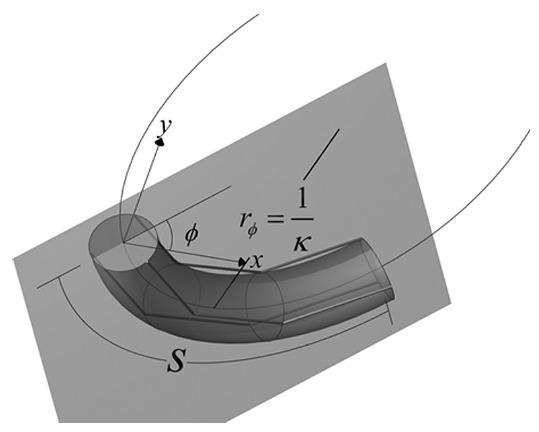
\includegraphics[width=\textwidth]{figures/multi_sec_manip.jpg}
		\end{column}
		\begin{column}{.68\linewidth}
			\centering
			\includegraphics[width=\textwidth]{figures/serret.jpg}
		\end{column}
	\end{columns}
	\footnotesize{Elephant Trunk Multi-sectional Continuum Model (left), and its Representation in the Serret-Frenet Frame.}
\end{frame}
\begin{frame}
	\frametitle{Pl{\"u}cker Coordinates Example}
	\begin{block}{Chasles' Theorem Applied to The Serret-Frenet Frame}
		Consider a spatial curve $\bm{S}$ on the elephant continuum trunk shown earlier. Suppose $\bm{S}$ is parameterized by its arc length $\bm{s} \in [0, 1]$. 
		For a point $\bm{x}=\left[x, y, z\right]^T$ on $\bm{S}$, the unit tangent vector at $s$ is $\bm{t}(s)=\bm{dx}/\bm{ds}$.
	\end{block}
	%	
	\begin{block}{Differential Kinematics and The Serret-Frenet Frame}
		 Denote by $\bm{n}$ the principal normal to $\bm{S}$ at $\bm{n}$; then we must have $\bm{b}=\bm{t}\times \bm{n}$ as the binormal. We say $(\bm{b},\bm{n})$ is the Pl{\"u}cker coordinate of the tangent $\bm{t}$.
	\end{block}
\end{frame}

\subsection{Force \& Wrench}
\begin{frame}
	\frametitle{Force}
	%	
	\begin{block}{Force}
		Net \textcolor{blue}{force} exerted on a body, 
		$\textcolor{red}{\bm{F}} = (f_x, f_y, f_z)$.
	\end{block}
	\begin{block}{Couple of Force}
		Suppose that $\bm{F}$ acts along a corkscrew axis. The resulting motion when $\bm{F}$ makes an infinitesimal rotation about its screw axis  is called its \textcolor{red}{couple}, $\mathfrak{C} = (c_x, c_y, c_z)$.
	\end{block}
	%	
\end{frame}

\begin{frame}
	\frametitle{Complete Wrench on a Screw}
	%	
	\begin{block}{Wrench}		
		A \textcolor{purple}{wrench} requires six 
		s \textcolor{magenta}{algebraic quantities} for its  \textcolor{red}{complete specification}:  \textcolor{blue}{five ($\{w_i\}_{i=1}^5$) specify the screw}, the \textcolor{cyan}{sixth (or its intensity)}, $w_6$, specifies the \textcolor{light-blue}{force's magnitude}.
	\end{block}
	%		
	\begin{block}{Couple's Moment}		
		The moment of the \textcolor{purple}{couple} is the product of the \textcolor{magenta}{intensity of the wrench} and the \textcolor{red}{ and the screw's pitch} i.e. $\alpha(\mathfrak{C}) = w_6 \times p_w$.
	\end{block}
	%	
\end{frame}

\begin{frame}
	\frametitle{Wrench on a Screw}
	%	
	\begin{block}{Wrench}
		Simple Definition: A \textcolor{brown}{force} and a \textcolor{cyan}{couple} both acting in a plane perpendicular to the force.
	\end{block}
	%
	\begin{definition}[Complete Definition]		
		The \textcolor{brown}{resultant canonical system of forces} acting on a rigid body, \textcolor{light-blue}{reduced to a resultant force on a point}, and acting along the \textcolor{red}{resultant couple} that is \textcolor{cyan}{perpendicular to the plane} in which the force acts is called \textcolor{blue}{the wrench}.
	\end{definition}
	%	
\end{frame}

\begin{frame}
	\frametitle{Wrench in Pl{\"u}cker Coordinates}
	%
	\begin{definition}[Wrench Coordinates]
		A six-vector, $\bm{w}$, related to the Pl{\"u}cker coordinates  parameterize a wrench vector i.e. $\bm{w}=\left[(w_1, w_2, w_3), (w_4, w_5, w_6)\right]$ or $\bm{w}=\left(\bm{f}, \bm{m}\right)$, where $\bm{f}=(w_1, w_2, w_3)$ and $\bm{m}=(w_4, w_5, w_6)$.
	\end{definition}
	%
	\begin{block}{Pl{\"u}cker Coordinates of a Wrench}
		\begin{align}
			b_1 &= w_1, \quad b_2 = w_2, \quad b_3 = w_3 \\
			c_1 &= w_4 - p \cdot s_1, \quad c_2 = w_5-p\cdot s_2, \quad c_3 = t_6 - p\cdot w_3.
		\end{align}
		%
	\end{block}
\end{frame}

\begin{frame}
	\frametitle{Wrench in Pl{\"u}cker Coordinates}
	%
	\begin{block}{Pitch of the Wrench}
		$p_t = \dfrac{w_1\,w_4 + w_2 \, w_5 + w_3\,w_6}{w_1^2+w_2^2+w_3^2}=\dfrac{\bm{f}\cdot \bm{m}}{\bm{f}\cdot \bm{f}}$.
	\end{block}
	%
	\begin{block}{Pitch of the Wrench}
		Expressed as a ratio of the \textcolor{magenta}{moment applied about a point on the axis} to the \textcolor{light-blue}{magnitude of the force applied}  along the wrench axis. 
	\end{block}	
	%
	\begin{block}{Wrench's Magnitude}
		$\|f\| = \sqrt{w_1^2 + w_2^2 + w_3^2}$ if $p_w = 0$ else $\|m\| = \sqrt{w_4^2 + w_5^2 + w_6^2}$ if $p_w = \infty$.
	\end{block}	
\end{frame}

\begin{frame}
	\frametitle{Wrenches and Fixed Movements}
%	\begin{block}{Pitch of a Wrench, $p_w$}
%		Acts along a (corkscrew) axis,  $p_w\bm{F}=\mathfrak{C}$.
%	\end{block}
	%
	\begin{block}{Pure Force}
		Let pitch be \textcolor{light-blue}{zero}. That which results is \textcolor{red}{pure force} along its screw axis.
	\end{block}
	
	\begin{block}{Pure Couple}
		Let pitch be \textcolor{magenta}{infinite}. That which results \textcolor{red}{cannot be a finite wrench}, \textcolor{cyan}{except the intensity be zero}, whereupon the \textcolor{brown}{wrench becomes a pure couple in a plane that is perpendicular to the screw}.
	\end{block}
\end{frame}


\begin{frame}
	\frametitle{Statics and Instantaneous Kinematics}
	%
	\begin{block}{Statics and kinematics}
		\begin{center}
			\begin{tabular}{||c | c||} 
				\hline
				\textbf{Statics} & \textbf{Instantaneous Kinematics}  \\ %[0.5ex] 
				\hline\hline
				Force,  $\bm{F}$ about $n$. & Infinitesimal rotation, $\bm{\omega}$ \\ 
				\hline
				Couple, $\mathfrak{C}$: [$\bm{F}$] $\times$ [$\ell$] & Infinitesimal translation, $\bm{t}$ \\
				\hline
				$p_w = \pm \mathfrak{C}/\bm{F}$ & Pitch of a Wrench, $\bm{w}$ \\
				\hline
				$\mid\bm{F} \mid$ & Intensity of Wrench \\
				\hline
			\end{tabular}
			\text{Dyname}: $(\bm{F}, \mathfrak{C})$. Credits: Pl{\"u}cker (1866), Routh (1892).
		\end{center}
	\end{block}
	
\end{frame}

\subsection{Screws in Pl{\"u}cker Coordinates}
\begin{frame}
	\frametitle{Pl{\"u}cker Coordinates Kinetics Quiz}
	%
	\begin{block}{Poinsot's Theorem Quiz on a  Force and its Moment}
		Suppose that a force $\bm{F}$  acts at the point $\bm{a}$ in the image of Frame \ref{fig:plucker}. What are the Pl{\"u}cker coordinates of the \textcolor{red}{line of force}?
	\end{block}
\end{frame}

\note{
	\begin{frame}
		%
		\begin{block}{Poinsot's Theorem Quiz on a  Force and its Moment}
			Imagine that a force $\bm{F}$ is acting at the point $\bm{a}$ in the image of Frame \ref{fig:plucker}. Suppose that $\bm{\tau}$ is torque acting along the normal to point $\bm{a}$.  Then $(\bm{f,\tau})$ are the Pl{\"u}cker  coordinates of the \textcolor{red}{line of force}.
		\end{block}
		%
		\begin{block}{Arithmetics on Screws}
			Scalar and vector arithmetic operations are valid on infinitesimal  screws e.g.
			\begin{align}
				c_1 \bm{s}_1 + c_2 \bm{s}_2 = 0 \text{ for } c_1, \, c_2 \neq 0 \text{ on screws } \bm{s}_1, \bm{s}_2.
			\end{align}
		\end{block}
	\end{frame}
}

\subsection{$\mathbb{R}^3$ Motions}

\begin{frame}
	\frametitle{Pl{\"u}cker Coordinates Kinetics Quiz}
	%
	\begin{block}{Poinsot's Theorem Quiz on a  Force and its Moment}
		Suppose that a force $\bm{F}$  acts at the point $\bm{a}$ in the image of Frame \ref{fig:plucker}. What are the Pl{\"u}cker coordinates of the \textcolor{red}{line of force}?
	\end{block}
\end{frame}

\begin{frame}
	\frametitle{Rigid Body Transformations}
	%
	\begin{block}{Translation of Point $\bm{q}$ between Two Frames}
		For a reference frame, $o_0 x_0 y_0$ and a moving coordinate frame, $o_1 x_1 y_1$, the translation of $\bm{q}$ is given as below:
	\end{block}
	\begin{columns}[]
		\begin{column}{.5\linewidth}
			\centering
			\includegraphics[width=\textwidth]{../Notes/figures/trans_coords.jpg}
		\end{column}
		\begin{column}{.5\linewidth}
			\begin{align}
				q^0 = \left( \begin{array}{c}
					q^0_x \\ q_y^0
				\end{array}
				\right), \quad
				%
				q^1 = \left( \begin{array}{c}
					q^1_x \\ q_y^1
				\end{array}
				\right) \nonumber
			\end{align}
		\end{column}
	\end{columns}
	%
	\begin{block}{Translation of Origin between Two Frames}
		\begin{align}
			o^0_1 = \left( \begin{array}{c}
				o^0_x \\ o^0_y
			\end{array}
			\right), \quad
			%
			o^1_0 = \left( \begin{array}{c}
				o^1_x \\ o^1_y
			\end{array}
			\right).
		\end{align}
	\end{block}
\end{frame}

\begin{frame}
	\frametitle{Rigid Body Transformations}
	%
	\begin{block}{Applications to Screws}
		Applies to Chasles' displacement theorem and Poinsot's force and couple transformations too.
	\end{block}
	%
	\begin{block}{Screw Transformations}
		\begin{align}
			\bm{t}^0_1 &= \left( \begin{array}{c}
				t^0_x \\  t^0_y %\\  t^0_z
			\end{array}
			\right),
			%
			\quad \bm{t}^1_1 = R(-\theta) q^0 \\
			%
		    \bm{t}^0_2 &= R(\theta) q^0, \quad \bm{t}^1_2 = \left( \begin{array}{c}
				t^1_x \\  t^1_y %\\  t^1_y
			\end{array}
			\right)
		\end{align}
		%
		where $\theta$ is the angle coordinate frame $o_1 x_1 y_1$ makes w.r.t $o_0 x_0 y_0$.
	\end{block}
\end{frame}

\begin{frame}
	\frametitle{Rotations in $\bb{R}^3$}
	%
	\begin{block}{Rotations in $\bb{R}^3$}
		Conventions: Bodies' \textcolor{blue}{orientations} are \textcolor{magenta}{measured along a corkscrew direction}, specified by a \textcolor{cyan}{local coordinate frame}. Thus, \textcolor{magenta}{relative orientation} is measured from the \textcolor{cyan}{local coordinate frame} to an \textcolor{magenta}{inertial coordinate frame}.
	\end{block}
	%
\end{frame}

\begin{frame}
	\frametitle{Direction Cosines}
	%
	\begin{columns}[]
		\begin{column}{.6\linewidth}
			\centering
			\includegraphics[width=\textwidth]{../Notes/figures/rotation_illus.jpg}
		\end{column}
		\begin{column}{.4\linewidth}
			\begin{block}{Conventions}
			 $I$: \textcolor{magenta}{Inertial frame}; $J$: \textcolor{cyan}{Body frame}.
				%
			$\bm{q}: (\bm{x}_{ij}, \bm{y}_{ij},\bm{z}_{ij}) \in \bb{R}^3$: coordinates of the \textcolor{purple}{principal axes} of $J$ relative to $I$.
			\end{block}
		\end{column}
	\end{columns}
\end{frame}


\begin{frame}
	\frametitle{Rotation Matrix from Direction Cosines}
	\begin{block}{Rotation as Composition of Projections Between Frames}
		\begin{align}
			R_{ij} = \begin{bmatrix}
				\bm{x}_{ij} \quad  \bm{y}_{ij} \quad \bm{z}_{ij}
			\end{bmatrix} = \begin{bmatrix}
				r_{11} &  r_{12} & r_{13} \\
				r_{21} & r_{22} &  r_{23} \\
				r_{31} & r_{32} &  r_{33}
			\end{bmatrix}.
			\label{eq:rotation_compoz}
		\end{align}
	\end{block}
	
	\begin{block}{Rotation Matrix as Unit Axes' Dot Products}
		\begin{align}
			R_{ij} = \begin{bmatrix}
				\bm{x}_j \cdot \bm{x}_i & \bm{y}_j \cdot \bm{x}_i & \bm{z}_j \cdot \bm{x}_i \\
				%
				\bm{x}_j \cdot \bm{y}_i & \bm{y}_j \cdot \bm{y}_i & \bm{z}_j \cdot \bm{y}_i \\
				%
				\bm{x}_j \cdot \bm{z}_i & \bm{y}_j \cdot \bm{z}_i & \bm{z}_j \cdot \bm{z}_i 
			\end{bmatrix}.
			\label{eq:direction_cosines}
		\end{align}
	\end{block}
\end{frame}

\begin{frame}
	\frametitle{Rotation Matrix from Direction Cosines}
	\begin{block}{Rotation Matrices are Direction Cosines!}
		$\bm{x}_j \cdot \bm{x}_i = \cos(\measuredangle\left(\bm{x}_j, \bm{x}_i\right)), \quad 	\bm{y}_j \cdot \bm{x}_i = \cos(\measuredangle\left(\bm{y}_j, \bm{x}_i\right)), \cdots$
		
		$\cdots, \bm{y}_j \cdot \bm{z}_i = \cos(\measuredangle\left(\bm{y}_j, \bm{z}_i\right)), \quad 	\bm{z}_j \cdot \bm{z}_i = \cos(\measuredangle\left(\bm{z}_j, \bm{z}_i\right)).$
	\end{block}
	
	\begin{block}{Properties of Rotation Matrices}
		Rows of $R_{ij}$ are the \textcolor{magenta}{unit vector} coordinates of $I$  in the frame $J$ so that 
		%
		\begin{align}
			R_{ij} =  R_{ji}^{-1} = R_{ji}^T.
		\end{align}
		%
		That is, the \textcolor{blue}{inverse of the rotation matrix is equal to its transpose}. 
	\end{block}
\end{frame}

\subsection{Special Orthogonal Properties}
\begin{frame}
	\frametitle{Special Orthogonal 3, SO(3)}
	\begin{block}{Orthogonal properties!}
			Observe: $\text{det }  \bm{R} = \bm{r}_1^T \cdot \left(\bm{r}_2 \times \bm{r}_3\right)$. In \textcolor{cyan}{corkscrew notation}, $\text{det }  \bm{R} = +1$ i.e. $\bm{r}_2 \times \bm{r}_3 = \bm{r}_1$ so that $\text{det }  \bm{R} = \bm{r}_1^T \cdot \bm{r}_1 = +1$. A matrix that satisfies the above property is said to \textcolor{light-blue}{possess a special orthogonal 3, denoted SO(3),  property}.
	\end{block}
	
	\begin{block}{SO(n) Property}
		Special orthogonal means $\text{det } \bm{R} = + 1$. The set of all SO matrices in $\bb{R}^{n\times n}$ is 
		%
		\begin{align}
			\text{SO(n)} = \{\bm{R}\in \bb{R}^{n\times n}: \bm{R}\cdot \bm{R}^T = \bm{I}, \text{det }\bm{R} = + 1\}.
		\end{align}
	\end{block}
\end{frame}

\begin{frame}
	\frametitle{Rotations on Vectors}
	\begin{columns}[]
		\begin{column}{.85\linewidth}
			\begin{block}{Rotating a Vector}
				Suppose that a point $p_j$ is on a frame $J$, then the vector that connects a point $q_j$ in the frame $J$ to $p_j$ is $v_j = q_j - p_j$. Now, the rotation matrix's action on $v_j$ is
				%
				\begin{align}
					\bm{R}_{ij}(v_j) := \bm{R}_{ij} q_j - \bm{R}_{ij} p_j = q_i - p_i = v_i.
				\end{align}
			\end{block}
		\end{column}
	\end{columns}
\end{frame}


\begin{frame}
	\frametitle{Planar Rotations}
	\begin{columns}[]
		\begin{column}{.5\linewidth}
			\begin{block}{Planar Rotations}
				Let the angle of rotation between the two coordinate frames be $\theta$. Then,
			\begin{align}
				R_1^0 = \left(\begin{array}{cc}
					x_1^0 \,\,| & y_1^0
				\end{array}\right)
			\end{align}
			\end{block}
		\end{column}
		\begin{column}{.5\linewidth}
			\centering
			\includegraphics[width=\textwidth]{../Notes/figures/rotation_illus.jpg}
		\end{column}
	\end{columns}
	
	\begin{columns}[]
		\begin{column}{.5\linewidth}
			\begin{block}{Planar Rotations}
				It follows that
				\begin{align}
					R = \left(\begin{array}{cc}
						\cos \alpha & -\sin \alpha \\ \sin \alpha &  \cos \alpha
					\end{array}\right)
				\end{align}
			\end{block}
		\end{column}
		\begin{column}{.5\linewidth}
			\centering
			\includegraphics[width=\textwidth]{../Notes/figures/planar_rot.jpg}
		\end{column}
	\end{columns}
\end{frame}


\begin{frame}
	\frametitle{Planar Rotations}
			\begin{block}{Planar Rotations via Direction Cosines}
				\begin{align}
					R_1^0 &= \begin{bmatrix}
						\bm{x}_0 \cdot \bm{x}_1 & \bm{y}_1 \cdot \bm{x}_0 \\
						%
						\bm{x}_0 \cdot \bm{y}_1 & \bm{y}_1 \cdot \bm{y}_0
					\end{bmatrix} =  \begin{bmatrix}
					cos \alpha &  -cos(\pi/2 - \alpha) \\
					%
					cos(\pi/2 - \alpha) & cos \alpha
				\end{bmatrix} \nonumber \\
			%
		&=  \begin{bmatrix}
		cos \alpha &   - \sin \alpha  \\
		%
		\sin \alpha  & cos \alpha
	\end{bmatrix}.
				\end{align}
			\end{block}
		\footnotesize{Projection of $y_1$ on $x_0$ is negative because of our adopted right-handed frame.}
\end{frame}

\subsection{Composition of Rotations}
\begin{frame}
	\frametitle{Composition of Rotations}
			\begin{block}{Rotations Composition}
				Let the \textcolor{cyan}{relative orientation} of a frame $K$  to a frame $J$ be $\bm{R}_{jk}$, and let frame $J$'s  \textcolor{cyan}{relative orientation} to frame $I$ be $\bm{R}_{ij}$, then the \textcolor{cyan}{relative orientation} of frame $K$  w.r.t $I$ is 
				%
				\begin{align}
					\bm{R}_{ik} = \bm{R}_{ij} \cdot \bm{R}_{jk}.
				\end{align} 
			\end{block}
		
		\begin{block}{Rotations Composition}
			Equivalent to \textcolor{brown}{rotating $J$ relative to frame $I$ according to $\bm{R}_{ij}$}; then \textcolor{magenta}{aligning frame $J$  to $K$}, we \textcolor{light-blue}{rotate $K$ relative to $I$ according to $\bm{R}_{jk}$}. This frame relative to which rotation occurs is termed the \textcolor{light-red}{current frame}. 
		\end{block}
\end{frame}


\begin{frame}
	\frametitle{Composition of Rotations About A Current Axis}
	\begin{block}{Composition of Rotations About A Current Axis}
		%
		\centering
		\includegraphics[width=1\textwidth]{../Notes/figures/compoz.jpg}
	\end{block}
\end{frame} 

\begin{frame}
	\frametitle{Composition of Rotations About A Current Axis}
	\begin{block}{Compositions}
		\begin{align}
			\bm{R} &= \bm{R}_{x, \theta} \bm{R}_{z, \psi} 
			%
			= \left(\begin{array}{ccc}
				1 & 0 & 0 \\
				0 & c_\theta & -s_\theta \\
				0 & s_\theta & c_\theta
			\end{array}\right) 
			%
			\cdot
			%
			\left(\begin{array}{ccc}
				c_\psi & -s_\psi & 0 \\
				s_\psi & c_\psi & 0 \\
				0 & 0 & 1
			\end{array}\right) \\
			%
			\bm{R} &= \left(\begin{array}{ccc}
				c_\psi & -s_\psi & 0 \\
				0 & c_\theta c_\psi &  -s_\theta \\
				s_\theta s_\psi & s_\theta c_\psi & c_\theta 
			\end{array}\right)
		\end{align}
		%
		\footnotesize{Notice how the order of multiplication is carried out, owing to the axis about which we are making the transformation.} 
	\end{block}
\end{frame} 

\begin{frame}
	\frametitle{Composition of Rotations About A Current Axis}
	\begin{block}{Skew Symmetry Operations}
		%
		What happens when the \textcolor{red}{order of multiplication is reversed}?
	\end{block}
	
%	\begin{block}{Skew Symmetry}
%		%
%		Turns out \textcolor{light-blue}{going from rotations about a current frame} to a \textcolor{blue}{fixed axis} and \textcolor{brown}{rotations from a fixed axis} to a \textcolor{light-red}{current frame} is equivalent to \textcolor{purple}{skew-symmetric operations on matrices} i.e. 
%		\begin{align}
%			\bm{R}_{x, \theta} \bm{R}_{z, \psi}  =  \left(\bm{R}_{z, \psi} \bm{R}_{x, \theta}\right)^\wedge
%		\end{align}
%	\end{block}
\end{frame} 


\begin{frame}
	\frametitle{Composition of Rotations}
	\begin{block}{Skew Symmetric Matrix}
		%
		\begin{align}
			(S)^\wedge = \left(\begin{array}{ccc}
				0 & -s_z & s_y \\
				s_z & 0 & -s_x \\
				-s_y & s_x & 0 
			\end{array}\right)
		\end{align}
	\end{block}

\begin{block}{Skew Symmetric Matrix}
%
Observe $s_{ij} = -s_{ji}$ for $i\neq j$ and $s_ii=0$
\end{block}
\end{frame}


\begin{frame}
	\frametitle{Composition of Rotations}
			\begin{block}{Pre-multiplication of Rotations}
				%
				A \textcolor{cyan}{rotation} about \textcolor{brown}{a fixed axis} requires a \textcolor{light-blue}{pre-multiplication}.
			\end{block}
		
		\begin{block}{Post-multiplication of Rotations}
			%
			A \textcolor{cyan}{rotation} about \textcolor{brown}{a current axis} necessitates a \textcolor{light-blue}{post-multiplication}.
		\end{block}
\end{frame}



\begin{frame}
	\frametitle{Rotations' Composition}
	\begin{columns}[]
		\begin{column}{.65\linewidth}
			\begin{block}{Rotations Composition}
				Suppose all axes of the inertial frame are successively rotated by $\beta$  around $x_0, y_0, z_0$ respectively. What is the transformation? Verify that (1) $R_{e, \beta} = I$ where $e$ is the axes about which we are rotating and $\beta$ is the angle of rotation; (2) The composition of rotations about $\beta$ and $\alpha$ in a successive manner implies that $R_{z, \beta}, R_{z, \alpha} = R_{z, \beta + \alpha}$, and (3) ${(R_{z, \beta})}^{-1} = R_{z, -\beta}$. 
			\end{block}
		\end{column}
		\begin{column}{.45\linewidth}
			\centering
			\includegraphics[width=\textwidth]{../Notes/figures/two_frames.jpg}
			\footnotesize{Relative orientation between two frames.}
		\end{column}
	\end{columns}
\end{frame}


\begin{frame}
	\frametitle{Euler Angles as Parameterization of Rotations}
	\begin{columns}[]
		\begin{column}{.95\linewidth}
			\centering
			\includegraphics[width=\columnwidth]{../Notes/figures/zyz.png}
			\footnotesize{Relative orientation between two frames.}
		\end{column}
	\end{columns}
\end{frame}

\begin{frame}
	\frametitle{Euler Angles as Parameterization of Rotations}
			\begin{block}{Euler ($ZYZ$) Angles}
				\begin{align}
					\bm{R}_{ij}(\alpha, \beta, \gamma) &= \bm{R}_z(\alpha) \bm{R}_y(\beta) \bm{R}_z(\gamma) \\
					%
					& = \begin{bmatrix}
						c_\alpha & -s_\alpha & 0 \\
						%
						s_\alpha & c_\alpha & 0 \\
						%
						0 & 0 & 1
					\end{bmatrix}
					%
					\begin{bmatrix}
						c_\theta  & 0 & s_\theta\\
						%
						0  & 1 & 0 \\
						%
						-s_\theta  & 0 & c_\theta 
					\end{bmatrix} \nonumber \\
					%
					&= \begin{bmatrix}
						c_\alpha c_\beta c_\gamma - s_\alpha s_\gamma & -c_\alpha c_\beta s_\gamma - s_\alpha c_\gamma & c_\alpha s_\beta \\
						%
						s_\alpha c_\beta c_\gamma + c_\alpha s_\gamma & -s_\alpha c_\beta s_\gamma + c_\alpha c_\gamma  & s_\alpha s_\beta \\
						%
						-s_\beta c_\gamma & s_\beta s_\gamma & c_\beta
					\end{bmatrix} 
					\label{eq:zyz}
				\end{align} 
			\end{block}
\end{frame}

\begin{frame}
	\frametitle{Euler Angles as Parameterization of Rotations}
	\begin{block}{Euler ($ZYZ$) Angles. Case $\sin(\beta)>0$}
	\begin{subequations}
		\begin{align}
			\beta &= \arctan 2(r_{33}, \sqrt{1 - r_{33}^2})  \label{eq:euler_a}\\
			\alpha &= \arctan 2(r_{23}/\sin \beta, r_{13}/\sin \beta) \label{eq:euler_b} \\
			\gamma &= \arctan 2 (r_{32}/\sin \beta, -r_{31}/\sin \beta)
		\end{align}
		\label{eq:euler}
	\end{subequations}
	%
	\footnotesize{where $\arctan2(y, x)$ determines the quadrant of the angle based on the sign of $x$ and $y$}.
	\end{block}
\end{frame}

\begin{frame}
	\frametitle{Euler Angles as Parameterization of Rotations}
	\begin{block}{Euler ($ZYZ$) Angles. Case $\sin(\beta)<0$}
	\begin{subequations}
		\begin{align}
			\beta &=  \arctan2(r_{33}, -\sqrt{1 - r_{33}^2})  \label{eq:euler_neg_a}\\
			\alpha &= \arctan 2(-r_{23}/\sin \beta, -r_{13}/\sin \beta) \label{eq:euler_neg_b} \\
			\gamma &= \arctan 2 (-r_{32}/\sin \beta, r_{31}/\sin \beta)
		\end{align}
		\label{eq:euler_neg}
	\end{subequations}
		%
		\footnotesize{\textcolor{red}{Euler angles are not unique} owing to the sign of the angle about which the $y$ axis rotates!}
	\end{block}
\end{frame}


\begin{frame}
	\frametitle{Other Axes Parameterization of Rotations}
	\begin{block}{Fick ($ZYX$), Helmholtz ($YZX$) Angles.}
		 We could \textcolor{red}{permute the order of rotation} such as rotating successively about \textcolor{cyan}{different axes}. Examples include \textcolor{blue}{successive rotations about $ZYX$ axes for the Fick angles} and \textcolor{brown}{successive rotations about $YZX$ axes for Helmholtz angles}.
	\end{block}
	
	\begin{block}{Fick ($ZYX$) and Helmholtz ($YZX$) Angles.}
		These avoid \textcolor{blue}{Euler angle} \textcolor{red}{singularities} at $\bm{R} = \bm{I}$. This does not preclude \textcolor{red}{singularities at other configurations}.
	\end{block}
\end{frame}


\begin{frame}
	\frametitle{Fick angles and Yaw, Pitch, and Roll Axes}
	\begin{columns}[]
		\begin{column}{.45\linewidth}
			\begin{block}{Fick angles}
				Otherwise called the yaw, pitch, and roll angles. $\bm{R}_{ij}$ found by rotating about the $x-$axis  (roll), then the $y-$axis (pitch), and finally the $z-$axis -- all in the body frame. 
			\end{block}
		\end{column}
		\begin{column}{.55\linewidth}
			\centering
			\includegraphics[width=\textwidth]{figures/yawpitchroll.jpg}
			\footnotesize{Aircraft Principal Axes in the right-hand frame. Courtesy of Wikimedia commons.}
		\end{column}
	\end{columns}
\end{frame}

\begin{frame}
	\begin{tcolorbox}[title=Summary of Parameterizations]
		Rotation matrices can be parameterized in one of many ways depending on our use case. The common examples of parameterizations are 
		%
		\begin{inparaenum}[\itshape (1)\upshape] \newline
			\item Axis-Angle representation; \newline
			\item Euler  angles ($ZYZ$) representation; \newline
			\item Fick  angles (\ie $ZYX$ or yaw, pitch and roll)  representation; \newline
			\item Helmholtz angles (or $YZX$) angles representation; and \newline
			\item Quaternions.
		\end{inparaenum}
		
	\end{tcolorbox}
\end{frame}
\lecture{Screw Theory}{Lecture IV}
\section{Screw Theory}
\begin{frame}
	\frametitle{Lecture IV Outline}
	\begin{tcolorbox}[coltitle=yellow!50!black,colframe=magenta!25,split=.2,title=Lecture IV Outline]
		Screws Theory and Rigid Body Transformations.
		\tcblower
		Screws (properly revisited): Chasles' and Poinsot's theorem; Displacement and Force screws; Pl{\"u}cker coordinates.
		\vspace{.2cm}
		\newline
		Wrench; Instantaneous screw axis; Couple; Adjoint maps; Velocity transformations -- in Body and Spatial Homogeneous Coordinates.
		\vspace{.2cm}
		\newline
		Group theory: The Lie algebra, motions in $\mathfrak{se}(3)$;, and the Lie Group. 
		\vspace{.2cm}
		\newline
		Manipulator kinematics: Brockett's exponential map formula. Paden-Kahan subproblems.Denavit-Hartenberg Conventions.
	\end{tcolorbox}
\end{frame}

\begin{frame}
	\frametitle{Rigid Body Motions as Screws}
	%
	\begin{block}{Rigid Body Motion as a Screw Motion}
		The motion of a \textcolor{red}{rigid body} is precisely the same as if it were attached to  the \textcolor{red}{nut of a literal mechanical screw}. Associated with the screw is its pitch.
	\end{block}	
	%
	\begin{definition}[Screw]
		That straight line with which a \textcolor{red}{definite linear magnitude} termed the pitch is associated is called the \textcolor{red}{screw}.
	\end{definition}
\end{frame}


\begin{frame}
	\frametitle{Screw as a Geometric Quantity}	
	%	
	\begin{block}{Pitch of a Screw}
		\textcolor{brown}{The rectilinear distance}  through which (a literal nut)  \textcolor{red}{nut is translated parallel to the axis of a screw}, while the nut is rotated through the \textcolor{cyan}{angular unit of circular measure} is termed the \textcolor{light-blue}{pitch}.
	\end{block}
	%
	\begin{block}{Pl{\"u}cker Coordinates}
		Let \textcolor{red}{$\bm{a}$} be a point on line $\bm{\ell}_0$. Let \textcolor{red}{$\bm{a}$}'s direction cosine vector (to be introduced shortly) be \textcolor{red}{$\bm{b}$}. Then, its binormal (moment) vector is \textcolor{red}{$\bm{c=a\times b}$}. We say the pair \textcolor{red}{$(\bm{b},\bm{c})$} is the \textcolor{blue}{Pl{\"u}cker Coordinates} of point  \textcolor{red}{$\bm{a}$ on axis} $\bm{\ell}_0$.
	\end{block}	
\end{frame}

\begin{frame}
	\frametitle{Screw in Pl{\"u}cker Coordinates}
	%
	\begin{columns}[b]
		\begin{column}{.67\columnwidth}
			\centering
			\begin{definition}[Screw Coordinates]
				Six-vector, $\bm{s}$, related to the Pl{\"u}cker coordinates, parameterize a screw i.e. $\bm{s}=\left(s_1, s_2, s_3, s_4, s_5, s_6\right)$.
			\end{definition}
		\end{column}
		
		\begin{column}{.3\columnwidth}
			\centering
			\includegraphics[width=\textwidth]{figures/plucker_coords.jpg}
		\end{column}
		\label{fig:plucker}
	\end{columns}
\end{frame}


\subsection{Displacement \& Twist}
\begin{frame}
	\frametitle{Screws and Pl{\"u}cker Coordinates}
	%
	\begin{block}{Screw axis and Pl{\"u}cker Coordinates}
		\begin{align}
			b_1 &= s_1, \quad b_2 = s_2, \quad b_3 = s_3; \\
			c_1 &= s_4 - p \cdot s_1, \quad c_2 = s_5-p\cdot s_2, \quad c_3 = s_6 - p\cdot s_3.
		\end{align}
	\end{block}
	%
	\begin{block}{Pitch in Pl{\"u}cker Coordinates}
		\begin{align}
			p &= \dfrac{s_1 \, s_4 + s_2 \, s_5 + s_3 \, s_6}{{s_1^2 + s_2^2 + s_3^2}}, \\
			\mid s \mid &= \sqrt{s_1^2 + s_2^2 + s_3^2} \quad \text{if } p \neq \infty, \\
			\mid s \mid &= \sqrt{s_4^2 + s_5^2 + s_6^2} \quad \text{if } p = \infty
		\end{align}
	\end{block}
\end{frame}


\begin{frame}
	\frametitle{Pitch and Magnitude of the screw}	
	\begin{block}{Pl{\"u}cker Coordinates' Direction Cosines}
		Suppose that 
		%\begin{align}
		$h = \sqrt{b_1^2+b_2^2+b_3^2}$.
		%\end{align}
		Then $(\bm{b}/h, \bm{c}/h)$ are respectively the direction cosines of the line, $l_0$ and its moment.
	\end{block}
	%
	\begin{block}{ Homogeneous Coordinates!}
		\textcolor{blue}{Pl{\"u}cker Coordinates} give six unit parameters of a point on a line. Pl{\"u}cker Coordinates are in \textcolor{red}{homogeneous coordinates}!
	\end{block}
\end{frame}

\begin{frame}
	\frametitle{Twist About a Screw (Axis)}
	%
	\begin{block}{Twist}
		A body's \textcolor{purple}{twist} about 
		s \textcolor{magenta}{screw} is a \textcolor{red}{uniform (infinitesimal) rotation} about the screw \textcolor{blue}{followed by a uniform (infinitesimal) translation} about an \textcolor{cyan}{axis parallel to the screw}, through \textcolor{magenta}{a distance that is the product of the pitch and the circular measure of rotation}.
	\end{block}	
	%
	\begin{block}{Twist}
		A \textcolor{purple}{twist} requires six 
		s \textcolor{magenta}{algebraic quantities} for its  \textcolor{red}{complete specification}:  \textcolor{blue}{five ($\{t_i\}_{i=1}^5$) specify the screw}, the \textcolor{cyan}{sixth (or its amplitude)} specifies the \textcolor{light-blue}{screw's rotaty angle}, $t_6$.
	\end{block}	
\end{frame}

\begin{frame}
	\frametitle{Twist in Pl{\"u}cker Coordinates}
	%
	\begin{definition}[Twist Coordinates]
		A six-vector, $\bm{t}$, related to the Pl{\"u}cker coordinates  parameterize a twist vector i.e. $\bm{t}=\left[(t_1, t_2, t_3), (t_4, t_5, t_6)\right]$ or $\bm{t}=\left(\bm{\omega}, \bm{v}\right)$, where $\bm{\omega}=(t_1, t_2, t_3)$ and $\bm{v}=(t_4, t_5, t_6)$.
	\end{definition}
	%
	\begin{block}{Pl{\"u}cker Coordinates of a Twist}
		\begin{align}
			b_1 &= t_1, \quad b_2 = t_2, \quad b_3 = t_3 \\
			c_1 &= t_4 - p \cdot s_1, \quad c_2 = t_5-p\cdot s_2, \quad c_3 = t_6 - p\cdot s_3.
		\end{align}
		%
	\end{block}
\end{frame}

\begin{frame}
	\frametitle{Twists in Pl{\"u}cker Coordinates}
	%
	\begin{block}{Pitch of the Twist}
		$p_t = \dfrac{t_1\,t_4 + t_2 \, t_5 + t_3\,t_6}{t_1^2+t_2^2+t_3^2}=\dfrac{\bm{\omega}\cdot \bm{v}}{\bm{\omega}\cdot \bm{\omega}}$.
	\end{block}
	%
	\begin{block}{Pitch of the Twist}
		Expressed as a ratio of the \textcolor{magenta}{magnitude of the velocity of a point on the twist axis} to the \textcolor{green}{magnitude of the angular velocity} about the twist axis. 
	\end{block}	
	%
	\begin{block}{Translation Distance}
		$d_t = t_6 \times p_t$.  The sign expresses the rotation's direction.
	\end{block}	
\end{frame}


\begin{frame}
	\frametitle{Twists and Fixed Movements}
	\begin{block}{Pure Rotation}
		Let pitch be \textcolor{light-blue}{zero}. That which results is but \textcolor{red}{pure rotation}.
	\end{block}
	
	\begin{block}{Pure Translation}
		Let pitch be \textcolor{magenta}{infinite}. That which results \textcolor{red}{cannot be a finite twist}, \textcolor{cyan}{except the amplitude be zero}, whereupon the \textcolor{brown}{twist becomes a pure translation parallel to the screw}.
	\end{block}
\end{frame}

%
\begin{frame}
	\frametitle{Curvilinear Displacement: Serret-Frenet Frame}
	\begin{columns}[]
		\begin{column}{.5\linewidth}
			\centering
			\includegraphics[width=\textwidth]{figures/multi_sec_manip.jpg}
		\end{column}
		\begin{column}{.68\linewidth}
			\centering
			\includegraphics[width=\textwidth]{figures/serret.jpg}
		\end{column}
	\end{columns}
	\footnotesize{Elephant Trunk Multi-sectional Continuum Model (left), and its Representation in the Serret-Frenet Frame.}
\end{frame}
\begin{frame}
	\frametitle{Pl{\"u}cker Coordinates Example}
	\begin{block}{Chasles' Theorem Applied to The Serret-Frenet Frame}
		Consider a spatial curve $\bm{S}$ on the elephant continuum trunk shown earlier. Suppose $\bm{S}$ is parameterized by its arc length $\bm{s} \in [0, 1]$. 
		For a point $\bm{x}=\left[x, y, z\right]^T$ on $\bm{S}$, the unit tangent vector at $s$ is $\bm{t}(s)=\bm{dx}/\bm{ds}$.
	\end{block}
	%	
	\begin{block}{Differential Kinematics and The Serret-Frenet Frame}
		Denote by $\bm{n}$ the principal normal to $\bm{S}$ at $\bm{n}$; then we must have $\bm{b}=\bm{t}\times \bm{n}$ as the binormal. We say $(\bm{b},\bm{n})$ is the Pl{\"u}cker coordinate of the tangent $\bm{t}$.
	\end{block}
\end{frame}

\subsection{Force \& Wrench}
\begin{frame}
	\frametitle{Force}
	%	
	\begin{block}{Force}
		Net \textcolor{blue}{force} exerted on a body, 
		$\textcolor{red}{\bm{F}} = (f_x, f_y, f_z)$.
	\end{block}
	\begin{block}{Couple of Force}
		Suppose that $\bm{F}$ acts along a corkscrew axis. The resulting motion when $\bm{F}$ makes an infinitesimal rotation about its screw axis  is called its \textcolor{red}{couple}, $\mathfrak{C} = (c_x, c_y, c_z)$.
	\end{block}
	%	
\end{frame}

\begin{frame}
	\frametitle{Complete Wrench on a Screw}
	%	
	\begin{block}{Wrench}		
		A \textcolor{purple}{wrench} requires six 
		s \textcolor{magenta}{algebraic quantities} for its  \textcolor{red}{complete specification}:  \textcolor{blue}{five ($\{w_i\}_{i=1}^5$) specify the screw}, the \textcolor{cyan}{sixth (or its intensity)}, $w_6$, specifies the \textcolor{light-blue}{force's magnitude}.
	\end{block}
	%		
	\begin{block}{Couple's Moment}		
		The moment of the \textcolor{purple}{couple} is the product of the \textcolor{magenta}{intensity of the wrench} and the \textcolor{red}{ and the screw's pitch} i.e. $\alpha(\mathfrak{C}) = w_6 \times p_w$.
	\end{block}
	%	
\end{frame}

\begin{frame}
	\frametitle{Wrench on a Screw}
	%	
	\begin{block}{Wrench}
		Simple Definition: A \textcolor{brown}{force} and a \textcolor{cyan}{couple} both acting in a plane perpendicular to the force.
	\end{block}
	%
	\begin{definition}[Complete Definition]		
		The \textcolor{brown}{resultant canonical system of forces} acting on a rigid body, \textcolor{light-blue}{reduced to a resultant force on a point}, and acting along the \textcolor{red}{resultant couple} that is \textcolor{cyan}{perpendicular to the plane} in which the force acts is called \textcolor{blue}{the wrench}.
	\end{definition}
	%	
\end{frame}

\begin{frame}
	\frametitle{Wrench in Pl{\"u}cker Coordinates}
	%
	\begin{definition}[Wrench Coordinates]
		A six-vector, $\bm{w}$, related to the Pl{\"u}cker coordinates  parameterize a wrench vector i.e. $\bm{w}=\left[(w_1, w_2, w_3), (w_4, w_5, w_6)\right]$ or $\bm{w}=\left(\bm{f}, \bm{m}\right)$, where $\bm{f}=(w_1, w_2, w_3)$ and $\bm{m}=(w_4, w_5, w_6)$.
	\end{definition}
	%
	\begin{block}{Pl{\"u}cker Coordinates of a Wrench}
		\begin{align}
			b_1 &= w_1, \quad b_2 = w_2, \quad b_3 = w_3 \\
			c_1 &= w_4 - p \cdot s_1, \quad c_2 = w_5-p\cdot s_2, \quad c_3 = t_6 - p\cdot w_3.
		\end{align}
		%
	\end{block}
\end{frame}

\begin{frame}
	\frametitle{Wrench in Pl{\"u}cker Coordinates}
	%
	\begin{block}{Pitch of the Wrench}
		$p_t = \dfrac{w_1\,w_4 + w_2 \, w_5 + w_3\,w_6}{w_1^2+w_2^2+w_3^2}=\dfrac{\bm{f}\cdot \bm{m}}{\bm{f}\cdot \bm{f}}$.
	\end{block}
	%
	\begin{block}{Pitch of the Wrench}
		Expressed as a ratio of the \textcolor{magenta}{moment applied about a point on the axis} to the \textcolor{light-blue}{magnitude of the force applied}  along the wrench axis. 
	\end{block}	
	%
	\begin{block}{Wrench's Magnitude}
		$\|f\| = \sqrt{w_1^2 + w_2^2 + w_3^2}$ if $p_w = 0$ else $\|m\| = \sqrt{w_4^2 + w_5^2 + w_6^2}$ if $p_w = \infty$.
	\end{block}	
\end{frame}

\begin{frame}
	\frametitle{Wrenches and Fixed Movements}
	%	\begin{block}{Pitch of a Wrench, $p_w$}
		%		Acts along a (corkscrew) axis,  $p_w\bm{F}=\mathfrak{C}$.
		%	\end{block}
	%
	\begin{block}{Pure Force}
		Let pitch be \textcolor{light-blue}{zero}. That which results is \textcolor{red}{pure force} along its screw axis.
	\end{block}
	
	\begin{block}{Pure Couple}
		Let pitch be \textcolor{magenta}{infinite}. That which results \textcolor{red}{cannot be a finite wrench}, \textcolor{cyan}{except the intensity be zero}, whereupon the \textcolor{brown}{wrench becomes a pure couple in a plane that is perpendicular to the screw}.
	\end{block}
\end{frame}


\begin{frame}
	\frametitle{Statics and Instantaneous Kinematics}
	%
	\begin{block}{Statics and kinematics}
		\begin{center}
			\begin{tabular}{||c | c||} 
				\hline
				\textbf{Statics} & \textbf{Instantaneous Kinematics}  \\ %[0.5ex] 
				\hline\hline
				Force,  $\bm{F}$ about $n$. & Infinitesimal rotation, $\bm{\omega}$ \\ 
				\hline
				Couple, $\mathfrak{C}$: [$\bm{F}$] $\times$ [$\ell$] & Infinitesimal translation, $\bm{t}$ \\
				\hline
				$p_w = \pm \mathfrak{C}/\bm{F}$ & Pitch of a Wrench, $\bm{w}$ \\
				\hline
				$\mid\bm{F} \mid$ & Intensity of Wrench \\
				\hline
			\end{tabular}
			\text{Dyname}: $(\bm{F}, \mathfrak{C})$. Credits: Pl{\"u}cker (1866), Routh (1892).
		\end{center}
	\end{block}
	
\end{frame}

\subsection{Screws in Pl{\"u}cker Coordinates}
\begin{frame}
	\frametitle{Pl{\"u}cker Coordinates Kinetics Quiz}
	%
	\begin{block}{Poinsot's Theorem Quiz on a  Force and its Moment}
		Suppose that a force $\bm{F}$  acts at the point $\bm{a}$ in the image of Frame \ref{fig:plucker}. What are the Pl{\"u}cker coordinates of the \textcolor{red}{line of force}?
	\end{block}
\end{frame}

\note{
	\begin{frame}
		%
		\begin{block}{Poinsot's Theorem Quiz on a  Force and its Moment}
			Imagine that a force $\bm{F}$ is acting at the point $\bm{a}$ in the image of Frame \ref{fig:plucker}. Suppose that $\bm{\tau}$ is torque acting along the normal to point $\bm{a}$.  Then $(\bm{f,\tau})$ are the Pl{\"u}cker  coordinates of the \textcolor{red}{line of force}.
		\end{block}
		%
		\begin{block}{Arithmetics on Screws}
			Scalar and vector arithmetic operations are valid on infinitesimal  screws e.g.
			\begin{align}
				c_1 \bm{s}_1 + c_2 \bm{s}_2 = 0 \text{ for } c_1, \, c_2 \neq 0 \text{ on screws } \bm{s}_1, \bm{s}_2.
			\end{align}
		\end{block}
	\end{frame}
}


\begin{frame}
	\frametitle{Pl{\"u}cker Coordinates Kinetics Quiz}
	%
	\begin{block}{Poinsot's Theorem Quiz on a  Force and its Moment}
		Suppose that a force $\bm{F}$  acts at the point $\bm{a}$ in the image of Frame \ref{fig:plucker}. What are the Pl{\"u}cker coordinates of the \textcolor{red}{line of force}?
	\end{block}
\end{frame}


\subsection{Group Theory Connections}
\begin{frame}
	\frametitle{Group Theory Review}
	\begin{block}{The Euclidean Motion}
		Let $\mathbb{E}^3$ denote the ordinary Cartesian 3-space that admits the standard inner product 
		%
		\begin{align}
			\langle x, y \rangle = \sum_i x_i \, y_i.
		\end{align}
	\end{block}

	\begin{block}{Transformations}
		The set of all \textcolor{brown}{length-preserving transformations} in $\mathbb{E}^3$ shall be denoted by $\mathbb{E}(3) \in \mathbb{R}^6$ \ie the family of \textcolor{cyan}{translations and rotations}\footnote{Rotations in $\mathbb{E}^3$ are not necessarily proper.}.
	\end{block}
\end{frame}


\begin{frame}
	\frametitle{Group Transformation Isomorphism}
	\begin{block}{Brockett, 1990}
		\textcolor{brown}{Euclidean transformation under group composition} and  \textcolor{cyan}{Euclidean transformation under group multiplication} preserve the \textcolor{red}{isomorphic property}.
	\end{block}
	
	\begin{block}{Example: Affine Euclidean Transformations}
		$\bm{q}$ defines a \textcolor{brown}{Euclidean} \textcolor{light-blue}{affine transformation} $\bm{q} = \rot \bm{x} + \bm{d}$ \text{ if } $\langle \rot, \rot^T\rangle = \identity$ for $(\bm{q}, \bm{d}) \in \reline^3$. Now, suppose $\bm{q} = \rot_1 \bm{x} + \bm{d}_1$ and $\bm{p} = \rot_2 \bm{q} + \bm{d}_2$, then $\bm{p} = \rot_2 \rot_1\bm{x}+ \bm{d}_2$. %and $\bm{p} = \rot_2 \bm{q} + \bm{d}_2$
	\end{block}
\end{frame}


\begin{frame}
	\frametitle{Group Transformation Isomorphism}
	\begin{block}{Example: Euclidean Transformation Identity}
		\begin{align}
			\left(
			\begin{array}{cc}
				\rot_2 & \bm{d}_2 \\
				0 & 1
			\end{array}
			\right)
			\left(
			\begin{array}{cc}
				\rot_1 & \bm{d}_1 \\
				0 & 1
			\end{array}
			\right) = 
			\left(
			\begin{array}{cc}
				\rot_2 \rot_1 & \rot_2\bm{d}_1 + \bm{d}_2 \\
				0 & 1
			\end{array}
			\right)
		\end{align}
	\end{block}

	\begin{block}{The isomorphic property (Brockett, 1990)}
		That matrices of the form (SE(3) matrices):
		%\begin{align}
		$	\left(
			\begin{array}{cc}
				\rot & \bm{d} \\
				0 & 1
			\end{array}
			\right) $
		%\end{align}
	are isomorphic.
	\end{block}
\end{frame}

\begin{frame}
	\frametitle{The General Linear Group}
	\begin{block}{$SO(3)$ as a General Linear Group}
		The \textcolor{brown}{special orthogonal group, $\orthoggroup$,} is a \textcolor{blue}{subgroup} of the \textcolor{magenta}{general linear group}
		%
		\begin{align}
			\orthoggroup = \{\rot \in GL(n, \mathbb{R}): \rot \, \rot^T = \identity, \text{det } \rot = \identity \}.
		\end{align}
	\end{block}
\end{frame}

\begin{frame}
	\frametitle{The Lie Group}
	
	\begin{block}{The Lie Group}
		A group with a \textcolor{brown}{topology operation on its set of elements} such that the group can be given the \textcolor{blue}{structure of a differential manifold} with the property that \textcolor{magenta}{group multiplication and inversion} is \textcolor{blue}{continuous} is called a \textcolor{brown}{Lie group}.
	\end{block}
	
	\begin{block}{The Special Euclidean Matrix Group, $\liegroup(3)$}
		$\liegroup(3)$ is a \textcolor{brown}{differentiable manifold}, comprised of all the \textcolor{cyan}{translations} and \textcolor{blue}{proper rotations} that \textcolor{red}{moves a body from one point to another} in the ordinary cartesian 3-space $\textbf{E}^3$.
	\end{block}
\end{frame}

\begin{frame}
	\frametitle{The Lie Group}	
	\begin{block}{The Special Euclidean Matrix Group, $\liegroup(3)$}
		\begin{align}
			g = \begin{bmatrix}
				\bm{R} & \bm{d} \\ \bm{0}^T & 1
			\end{bmatrix}; g \in \liegroup(3).
			\label{eq:rigid_trans}
		\end{align}
	\end{block}
\end{frame}

\begin{frame}
	\frametitle{The Lie Group}	
	\begin{block}{The Special Euclidean Matrix Group, $\liegroup(3)$}
		\begin{align}
			\liegroup(3) = \{(\rot, d): \rot \in \orthoggroup, d \in \reline^3 \}:=\orthoggroup \times \reline^3.
			\label{eq:se3_rep}
		\end{align}
		 \footnotesize{I have followed \textcolor{brown}{Chasles' notation}, who posited that \textcolor{cyan}{any rigid motion can be formed via a rotation}, \textcolor{brown}{followed by a translation}, and that \textcolor{purple}{the rotation and the translation commute} i.e. $\rot \, d = d$}.
	\end{block}

	\begin{block}{The Special Euclidean Matrix Group, $\liegroup(3)$}
		\footnotesize{Note: Most authors' notation follow \textcolor{red}{Euclid's theorem} i.e. any rigid motion is a \textcolor{magenta}{translation} followed by a \textcolor{cyan}{rotation about an axis} that \textcolor{blue}{passes through a pre-specified (fixed) point}.}	
		\begin{align}
			\liegroup(3) = \{(d, \rot):  d \in \reline^3, \rot \in \orthoggroup 	\}:=  \reline^3 \times \orthoggroup.
			\label{eq:se3_rep_euclid}
		\end{align}
	\end{block}
\end{frame}

\begin{frame}
	\frametitle{The Lie Group}		
	\begin{block}{The Special Euclidean Matrix Group, $\liegroup(3)$}
		\textcolor{blue}{Chasles' notation} allows for \textcolor{purple}{motion representation} in form of \textcolor{red}{screw motions}.
	\end{block}
	
	\begin{block}{Commutativity of group operations on $\liegroup(3)$}
		\textcolor{cyan}{[Brockett, 1990]}: Equation \eqref{eq:se3_rep} %and \eqref{eq:se3_rep_euclid} 
		imply that the \textcolor{blue}{Lie group} is a \textcolor{magenta}{semidirect product of simple Lie subgroup of orthogonal transformations} and the \textcolor{red}{abelian Lie subgroup of all translations}.
	\end{block}
\end{frame}



\begin{frame}
	\frametitle{The Lie Algebra}	
	\begin{block}{The Lie Algebra, $\liealg(3)$}
		The \textcolor{cyan}{Lie algebra} is a \textcolor{brown}{vector space} $\hat{\bm{\xi}} $ with the \textcolor{magenta}{antisymmetric bilinear operation} $[,]: \hat{\bm{\xi}}  \times \hat{\bm{\xi}} \rightarrow \hat{\bm{\xi}} $ which satisfies the \textcolor{cyan}{Jacobi identity}, 
		\begin{align}
			[\hat{\bm{\xi}}_1, [\hat{\bm{\xi}}_2, \hat{\bm{\xi}}_3]] +[\hat{\bm{\xi}}_2, [\hat{\bm{\xi}}_3, \hat{\bm{\xi}}_1]] + [\hat{\bm{\xi}}_3, [\hat{\bm{\xi}}_1, \hat{\bm{\xi}}_2]] = 0.
		\end{align}
		\footnotesize{NB: $[,]$ is alternatively the \textcolor{blue}{Lie bracket notation with antisymmetry operation $[\hat{\bm{\xi}}_2, \hat{\bm{\xi}}_3] = -[\hat{\bm{\xi}}_3, \hat{\bm{\xi}}_2]$}.}
	\end{block}
\end{frame}


\begin{frame}
	\frametitle{The Lie Algebra Representation}	
	\begin{block}{The Lie Algebra Representation, $\liealg(3)$}
		The \textcolor{cyan}{Lie algebra} admits the following \textcolor{red}{homogeneous coordinates representation} for a point $q \in \reline^3$ on a \textcolor{magenta}{link that rotates with unit velocity $\omega$}, 
		\begin{align}
			\hat{\bm{\xi}} =  \left(\begin{array}{cc}
				\tilde{\omega} & v \\
				0 & 0
			\end{array}\right) \in \liealg(3), \,\bm{\xi}=\left(\omega^T, v^T\right)^T \in \reline^6
		\end{align}
		{where $v = -\omega \times q$.}
	\end{block}
\end{frame}

\begin{frame}
	\frametitle{The Lie Algebra Representation}	
	\begin{block}{The Lie Algebra Representation, $\liealg(3)$}
		Observe:  
		\begin{align}
			\tilde{\omega} =  \left(\begin{array}{ccc}
				0 & -\omega_z & \omega_y \\
				\omega_z & 0 & -\omega_x \\
				-\omega_y &  \omega_x & 0
			\end{array}\right) \equiv -\tilde{\omega}^T \in \mathfrak{so}(3)
		\end{align}
		{is the \textcolor{red}{skew-symmetric form of the velocity of the tip point}, $\omega \in \reline^3$.}
	\end{block}
\end{frame}

\begin{frame}
	\frametitle{The Lie Algebra Diffeomorphisms}	
	\begin{block}{Lie Representation Snippet}
		Observe:  
		\begin{align}
			\tilde{(\cdot)}_{SO(3)}: &\reline^3 \rightarrow \mathfrak{so}(3) \\
			\tilde{(\cdot)}_{SE(3)}: &\reline^6 \rightarrow \mathfrak{se}(3) 
		\end{align}
		$\tilde{\omega}(S)\in \liealg(3)$: e.g. \textcolor{blue}{Twist parameterization} of a curve, deformation, \textcolor{red}{screw}.
		
		${\omega}(S)\in \reline^6$: e.g. \textcolor{blue}{Motion vector} e.g. linear + angular velocities, axial, shear, bending, and torsion motion.
	\end{block}
\end{frame}


\begin{frame}
	\frametitle{The exponential map belongs to the Lie Group}	
	\begin{block}{The exponential map, $exp(\mathfrak{se}(3))$, is an element of $SE(3)$}
		Given $g:  \left(\begin{array}{cc}
			\rot(\theta) & \bm{d} \\
			0 & 1
		\end{array}\right) \in SE(3)$ there exists a $\tilde{\bm{\xi}}=(\tilde{\omega}, v) \in \mathfrak{se}(3)$, such that  $exp(\tilde{\bm{\xi}} \theta) \in SE(3)$\footnote{Proof in Murray and Sastry, Prop 2.8.}.
	\end{block}
	
	\begin{block}{The exponential map, $exp(\mathfrak{se}(3))$, is surjective onto $SE(3)$}
		Given $g:  \left(\begin{array}{cc}
			\rot(\theta) & \bm{d} \\
			0 & 1
		\end{array}\right) \in SE(3)$ there exists a $\left(\begin{array}{cc}
		\tilde{\omega} & \bm{d} \\
		0 & 0
	\end{array}\right); \tilde{\omega}=-\tilde{\omega}^T$, such that  $exp(\tilde{\omega}) =g$\footnote{Proof in Murray and Sastry, Prop 2.9.}.
	\end{block}
\end{frame}

\begin{frame}
	\frametitle{Chasles and Affine Transformations}	
	\begin{block}{Chasles Theorem and Affine Transformations}
		\begin{align}
			\left(
			\begin{array}{cc}
				\rot & \bm{d} \\
				0 & 1
			\end{array}
			\right) = \left(
			\begin{array}{cc}
				\identity & \bm{c} \\
				0 & 1
			\end{array}
			\right)
			%
			\left(
			\begin{array}{cc}
				\rot & \bm{d} \\
				0 & 1
			\end{array}
			\right)
		\end{align}
		with $\rot\, \bm{d}=\bm{d}$. Note $\langle \bm{c}, \bm{d}\rangle=0$ for $\bm{c}$ and $\bm{d}$ to be unique.
	\end{block}
\end{frame}


\begin{frame}
	\frametitle{Screm Motion and Exponential Map}	
	\begin{block}{Screw Motion and Exponential Map (Brockett, 1990)}
		Range and null space of a $\tilde{\omega}$ are orthogonal. Thus,
		%
		\begin{align}
			\left(\begin{array}{cc}
				\identity & \bm{c} \\
				0 & 1
			\end{array}\right)
			%			
			\left(\begin{array}{cc}
				\tilde{\omega} & \bm{d} \\
				0 & 0
			\end{array}\right)
			%			
			\left(\begin{array}{cc}
					\identity & -\bm{c} \\
					0 & 1
			\end{array}\right) = 
			%			
			\left(\begin{array}{cc}
				\tilde{\omega} & \bm{d}-\tilde{\omega}\bm{c} \\
				0 & 0
			\end{array}\right)
		\end{align}
		 establishes that every motion of the form $\left(\begin{array}{cc}
		 	\tilde{\omega} & \bm{d} \\
		 	0 & 0
		 \end{array}\right)\theta$ is a \textcolor{red}{screw motion w.r.t some origin}.
	\end{block}
\end{frame}


\begin{frame}
	\frametitle{Group Composition and Screws Connection}	
	\begin{block}{The Lie Algebra Representation, $\liealg(3)$}
		Observe:  
		\begin{align}
			\tilde{(\cdot)}_{SO(3)}: &\reline^3 \rightarrow \mathfrak{so}(3) \\
			\tilde{(\cdot)}_{SE(3)}: &\reline^6 \rightarrow \mathfrak{se}(3) 
		\end{align}
		$\tilde{\omega}(S)\in \liealg(3)$: \textcolor{blue}{Twist parameterization} of a curve, deformation, \textcolor{red}{screw}.
		
		${\omega}(S)\in \reline^6$: \textcolor{blue}{Motion vector} e.g. linear + angular velocities, axial, shear, bending, and torsion motion.
	\end{block}
\end{frame}

% ---- Bibliography ----
\bibliographystyle{../../Proposal/styles/bibtex/spmpsci_unsrt}
{
\tiny
\bibliography{../../../SRS/Continuum/biblio}
}
\end{document}
